\documentclass[dvipsnames]{fairmeta}

\title{The Llama 3 Herd of Models}

\author[1]{Llama Team, AI @ Meta}
\affiliation[1]{A detailed contributor list can be found in the appendix of this paper.}

\abstract{
Modern artificial intelligence (AI) systems are powered by foundation models.
This paper presents a new set of foundation models, called Llama 3.
It is a herd of language models that natively support multilinguality, coding, reasoning, and tool usage.
Our largest model is a dense Transformer with 405B parameters and a context window of up to 128K tokens.
This paper presents an extensive empirical evaluation of Llama 3.
We find that Llama 3 delivers comparable quality to leading language models such as GPT-4 on a plethora of tasks.
We publicly release Llama 3, including pre-trained and post-trained versions of the 405B parameter language model and our Llama Guard 3 model for input and output safety.
The paper also presents the results of experiments in which we integrate image, video, and speech capabilities into Llama 3 via a compositional approach.
We observe this approach performs competitively with the state-of-the-art on image, video, and speech recognition tasks.
The resulting models are not yet being broadly released as they are still under development.
}

\date{July 23, 2024}

\metadata[Website]{\url{https://llama.meta.com/}}

\usepackage{makecell}
\usepackage{siunitx}
\usepackage{framed}
\usepackage{pifont}
\usepackage{graphicx,subcaption}
\usepackage{pifont}
\usepackage{xspace}
\usepackage{nicematrix}
\usepackage{nicefrac}
\usepackage{wrapfig}
\newcommand{\rulesep}{\unskip\ \vrule\ }
\newcommand{\cmark}{\textcolor{ForestGreen}{\ding{51}}}
\newcommand{\xmark}{\textcolor{red}{\ding{55}}}

\begin{document}

\maketitle

\providecommand{\llama}{Llama\xspace}
\providecommand{\llamatwo}{Llama~2\xspace}
\providecommand{\llamathree}{Llama~3\xspace}
\providecommand{\TODO}[1]{{\color{red}[\textbf{TODO}: #1]}}
\providecommand{\mlc}{Multilingual\xspace}
\providecommand{\gpt}{GPT-4\xspace}
\providecommand{\gptp}{GPT-4\xspace}
\providecommand{\gpto}{GPT-4o\xspace}
\providecommand{\gptfourturbo}{GPT-4 Turbo\xspace}
\providecommand{\sonnet}{Claude 3.5 Sonnet\xspace}
\providecommand{\nemotron}{Nemotron 4 340B\xspace}
\providecommand{\mixtralbig}{Mixtral 8$\times$22B\xspace}
\providecommand{\gptthreedotfivet}{GPT-3.5 Turbo\xspace}
\providecommand{\gemmatwo}{Gemma 2 9B\xspace}
\providecommand{\mistralsmall}{Mistral 7B\xspace}
\providecommand*{\acc}[1]{\num[round-mode=places,round-precision=2]{#1}}


\section{Introduction}
Despite the well-recognized importance of training data in advancing the capabilities of large language models (LLMs)~\cite{brown2020language,kaplan2020scaling,Razeghi2022ImpactOP}, there is no agreed-upon mechanisms for crediting or compensating data providers. As LLMs are increasingly integrated into our society and economy, the absence of such mechanisms has aggravated a tension between data and model providers, exemplified by recent legal challenges involving major tech companies~\cite{jlversusalphabet,metz2022lawsuit}. In this atmosphere, data valuation, which quantifies the contribution of each training data to the model output, has been discussed as a potential technical solution for tackling these societal issues~\cite{fernandez2023data,ghorbani2019data,huang2023citation,jia2019towards,worledge2023unifying,zhao2023addressing}. 

At a high level, most data valuation algorithms interpret the model output as a coalition of its training data, and evaluate the contribution of each example based on its influence on the model output when included or excluded from the training dataset~\cite{ghorbani2019data,ilyas2022datamodels,koh2017understanding,kwon2021beta}. If an inclusion of a specific training example consistently improves model performance, high value can be assigned to this example for its contribution. However, applying existing data valuation methods to recent LLMs and their vast training datasets has faced significant scalability challenges to date. For instance, sampling-based methods, such as the Shapley value~\cite{ghorbani2019data,kwon2021beta} or Datamodels~\cite{ilyas2022datamodels}, require retraining the model multiple times with varied combinations of data subsets to directly model the effect of in/excluding each data. Unfortunately, such repeated retraining is hardly affordable even for small models, let alone LLMs. To overcome this issue, gradient-based methods, including influence functions~\cite{koh2017understanding,park2023trak}, approximate the effect of data in/exclusion on the model output using gradient information without costly retraining. Even so, scaling gradient-based methods to LLMs is hindered by prohibitive compute and memory costs originating in the high-dimensional nature of the gradient.

Consequently, the main objective of this work is to bridge the gap in scaling existing data valuation methods to recent LLMs and their vast training datasets. Toward this goal, we focus on influence functions \cite{koh2017understanding,park2023trak}, a representative gradient-based data valuation method, and significantly improve its scalability with an efficient gradient projection algorithm. We visualize the proposed data valuation system in Figure~\ref{fig:diagram}, and detail our technical contributions below:

\begin{figure}
    \centering
    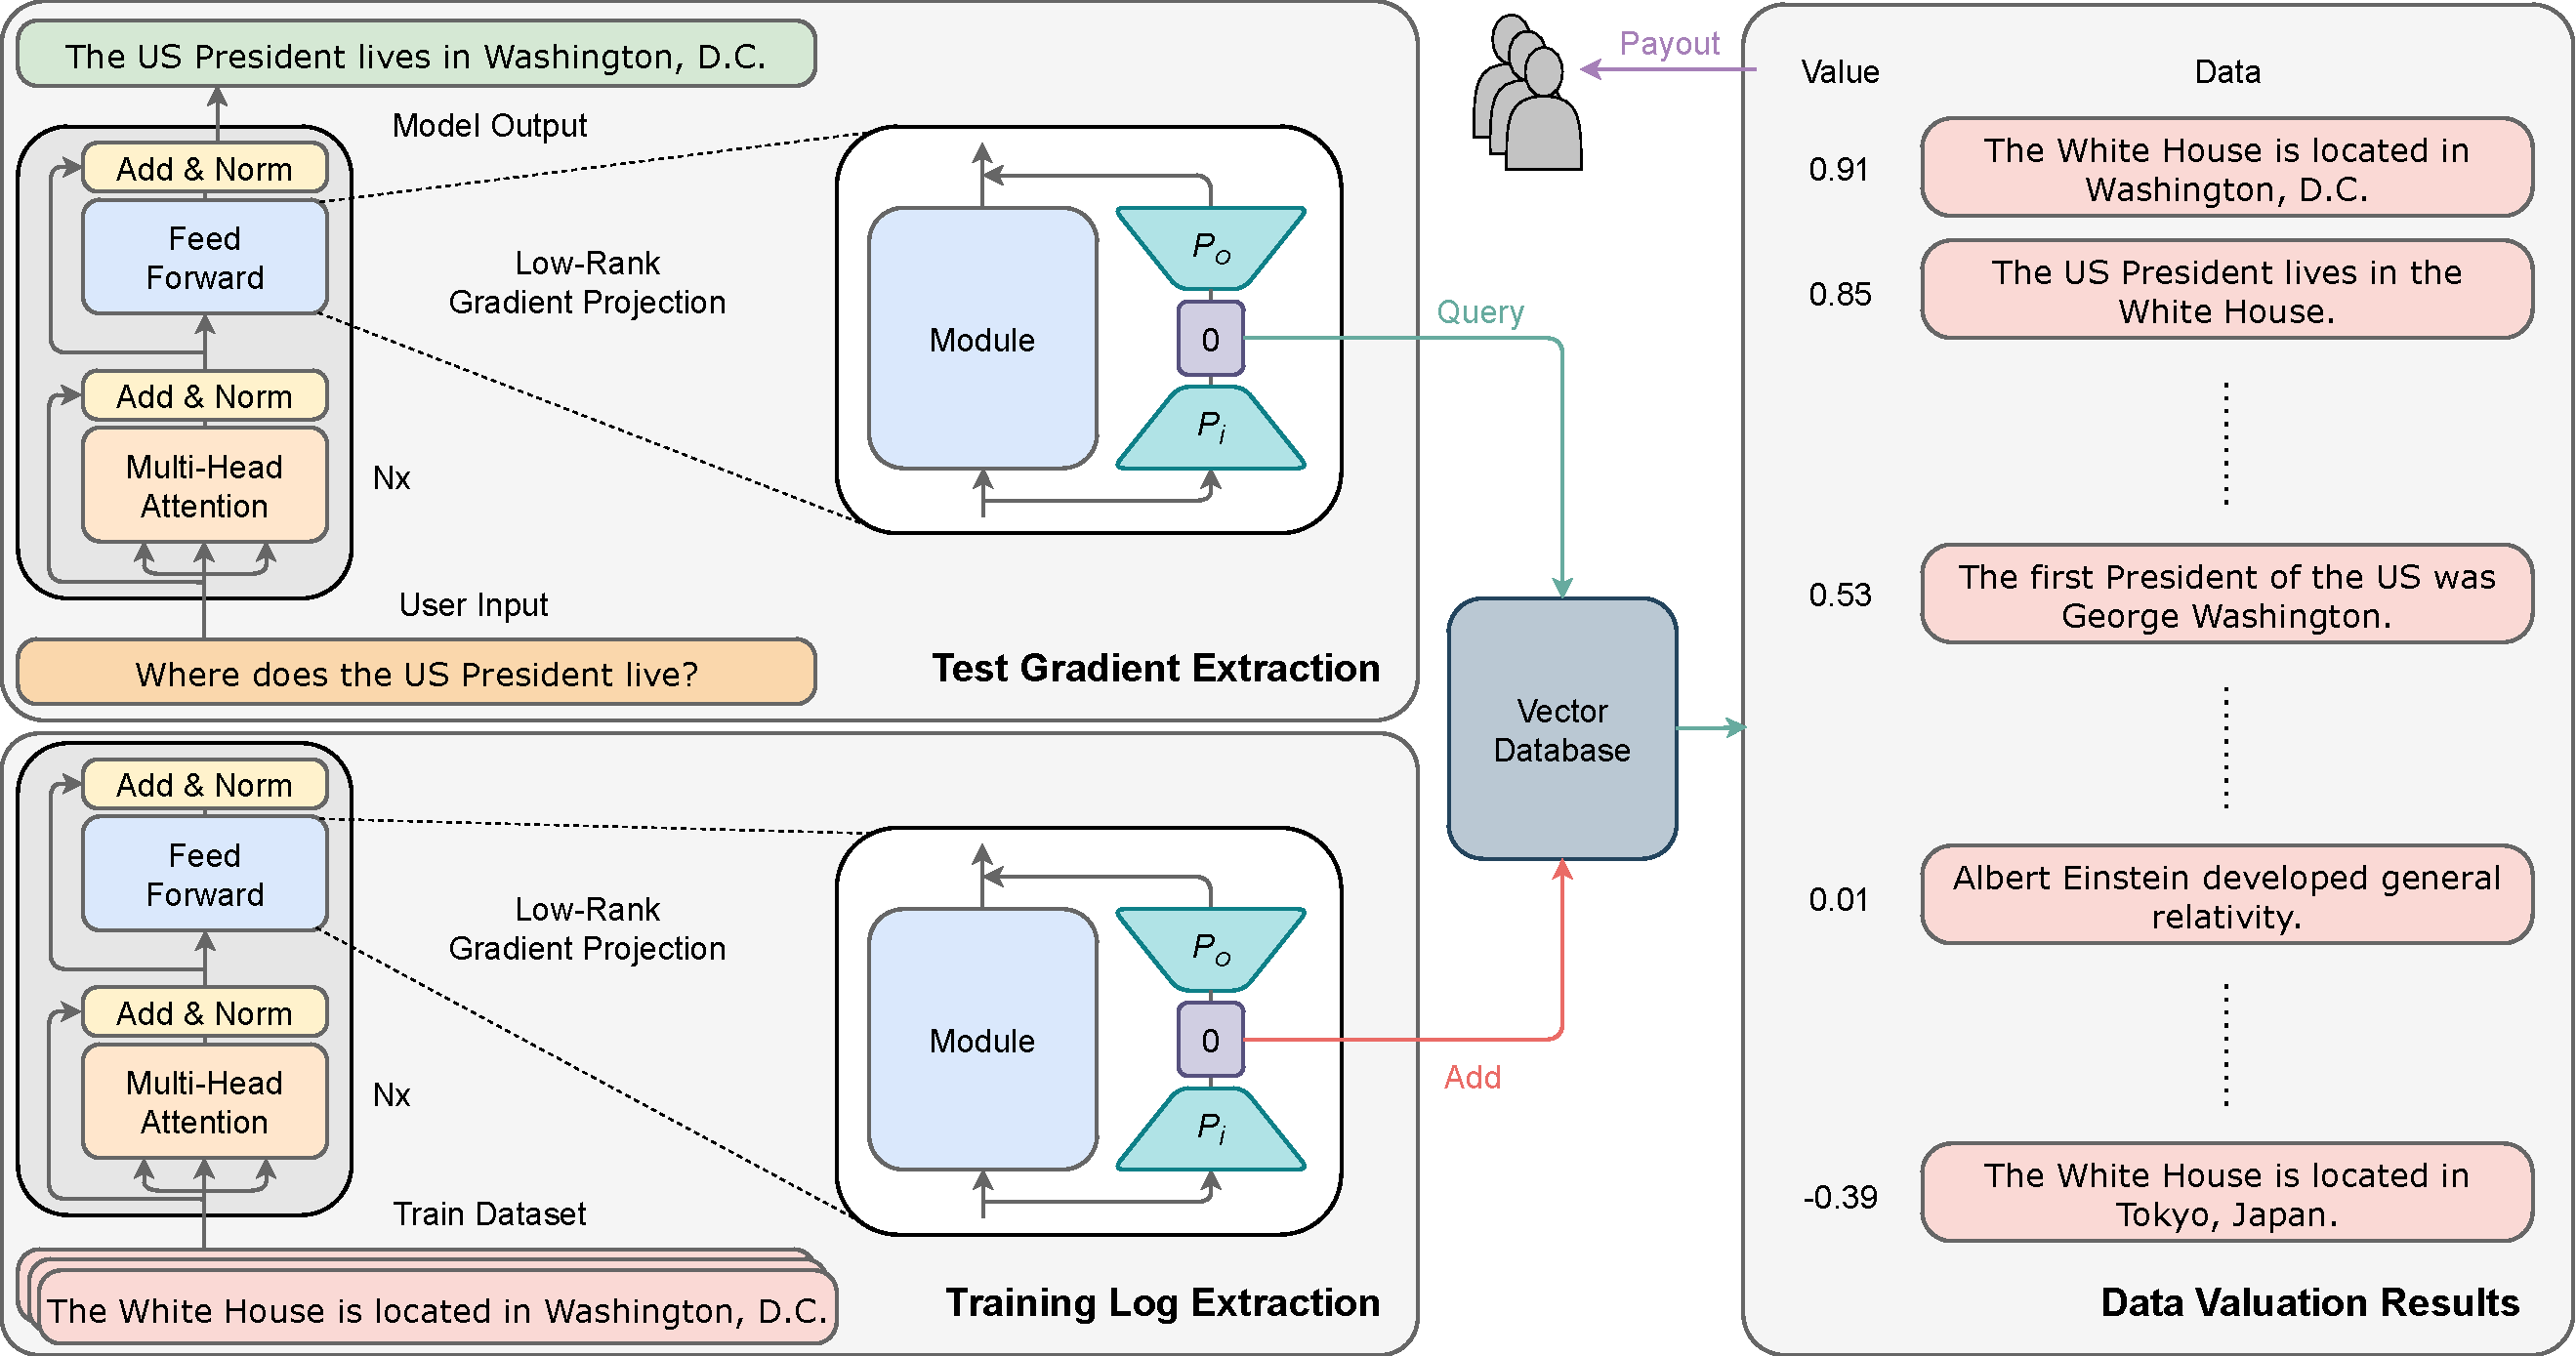
\includegraphics[width=0.94\textwidth]{figures/diagram_v7.pdf}
    \vskip -4pt
    \caption{Data valuation system architecture. \textbf{(Left Bottom)} We first extract the Hessian and gradients for all training data using efficient gradient projection \method\ and store them in a database. \textbf{(Left Top)} At test time, we similarly extract gradients and query the database. \textbf{(Right)} The database returns similarity scores with respect to training examples that can be used for data valuation/attribution.}
    \label{fig:diagram}
\end{figure}

\begin{itemize}[leftmargin=*,topsep=-2pt]
    \item Employing gradient structures in backpropagation, we develop a novel \textbf{lo}w-rank \textbf{gra}dient projection algorithm \method\ that improves space \& time complexity of gradient projection, a major scalability bottleneck in prior work~\cite{park2023trak,schioppa2022scaling}, from $O(nk)$ to $O(\sqrt{nk})$ where $n$ and $k$ are model and projection dimensions. Furthermore, \method\ directly computes projected gradients without materializing full gradients, enabling low GPU memory and high GPU utilization for improved efficiency. Lastly, we show that \method\ can be easily implemented with small add-on layers, similarly to LoRA~\cite{hu2021lora}.
    \item By interpreting a damping term in influence functions as a spectral gradient sparsification mechanism, we (1) offer a theoretical motivation of gradient projection approaches to influence functions and (2) derive a specialized PCA initialization scheme for \method.
    \item We introduce software named \software\ that (1) makes it \textit{simple} to convert existing training code into data valuation code, (2) is \textit{compatible} with various scalability tools and features in the LLM ecosystem, and (3) is \textit{extensible} to implement other data valuation or interpretability algorithms.
    \item In our data valuation experiments, \method\ demonstrates competitive accuracy against more costly baselines, while showing up to 6,500$\times$ increase in throughput and 5$\times$ reduction in GPU memory, when applied to Llama3-8B-Instruct~\cite{llama3modelcard} and the 1B-token dataset, compared to EKFAC influence \cite{grosse2023studying}, the state-of-the-art and only runnable baseline at this scale. We also observe that most valuable data identified by \method\ generally share qualitative similarities with the queried LLM output.
\end{itemize}
\begin{figure*}[t]
    \centering
    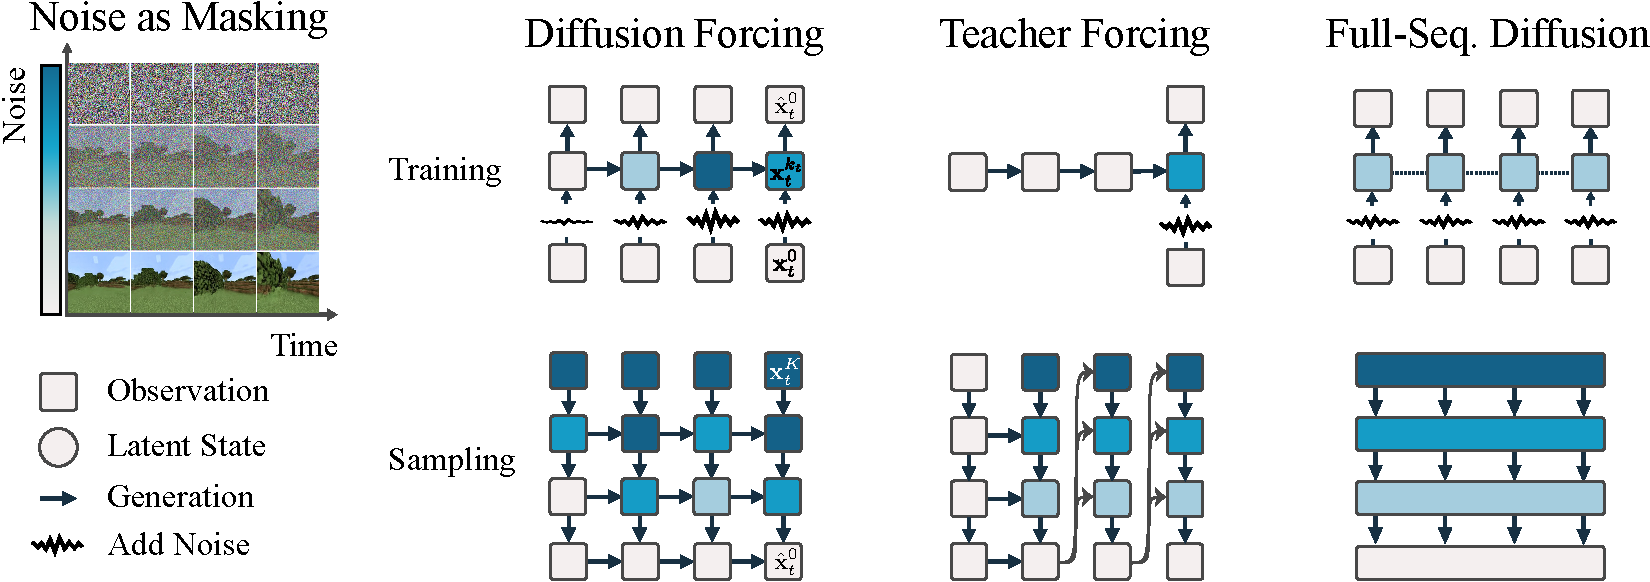
\includegraphics[width=\linewidth]{figures/pdf/Overview_best_guess.pdf}
    \caption{\textbf{Method Overview.} 
    Diffusion Forcing trains causal sequence neural networks (such as an RNN or a masked transformer) to denoise flexible-length sequences where each frame of the sequence can have a \emph{different} noise level.
    In contrast, next-token prediction models, common in language modeling, are trained to predict a single next token from a \emph{ground-truth} sequence (teacher forcing~\cite{teacher_forcing}), and full-sequence diffusion, common in video generation, train non-causal architectures to denoise all frames in a sequence at once with the \emph{same} noise level.
    \algo{} thus \emph{interleaves} the time axis of the sequence and the noise axis of diffusion, unifying strengths of both alternatives and enabling completely new capabilities (see Secs.~\ref{sec:zigzag_example},\ref{sec:method_decision_making}).
    }
    \label{fig:method}
    \vspace{-5pt}
\end{figure*}

\section{Training}

\begin{figure}[ht]
\begin{center}
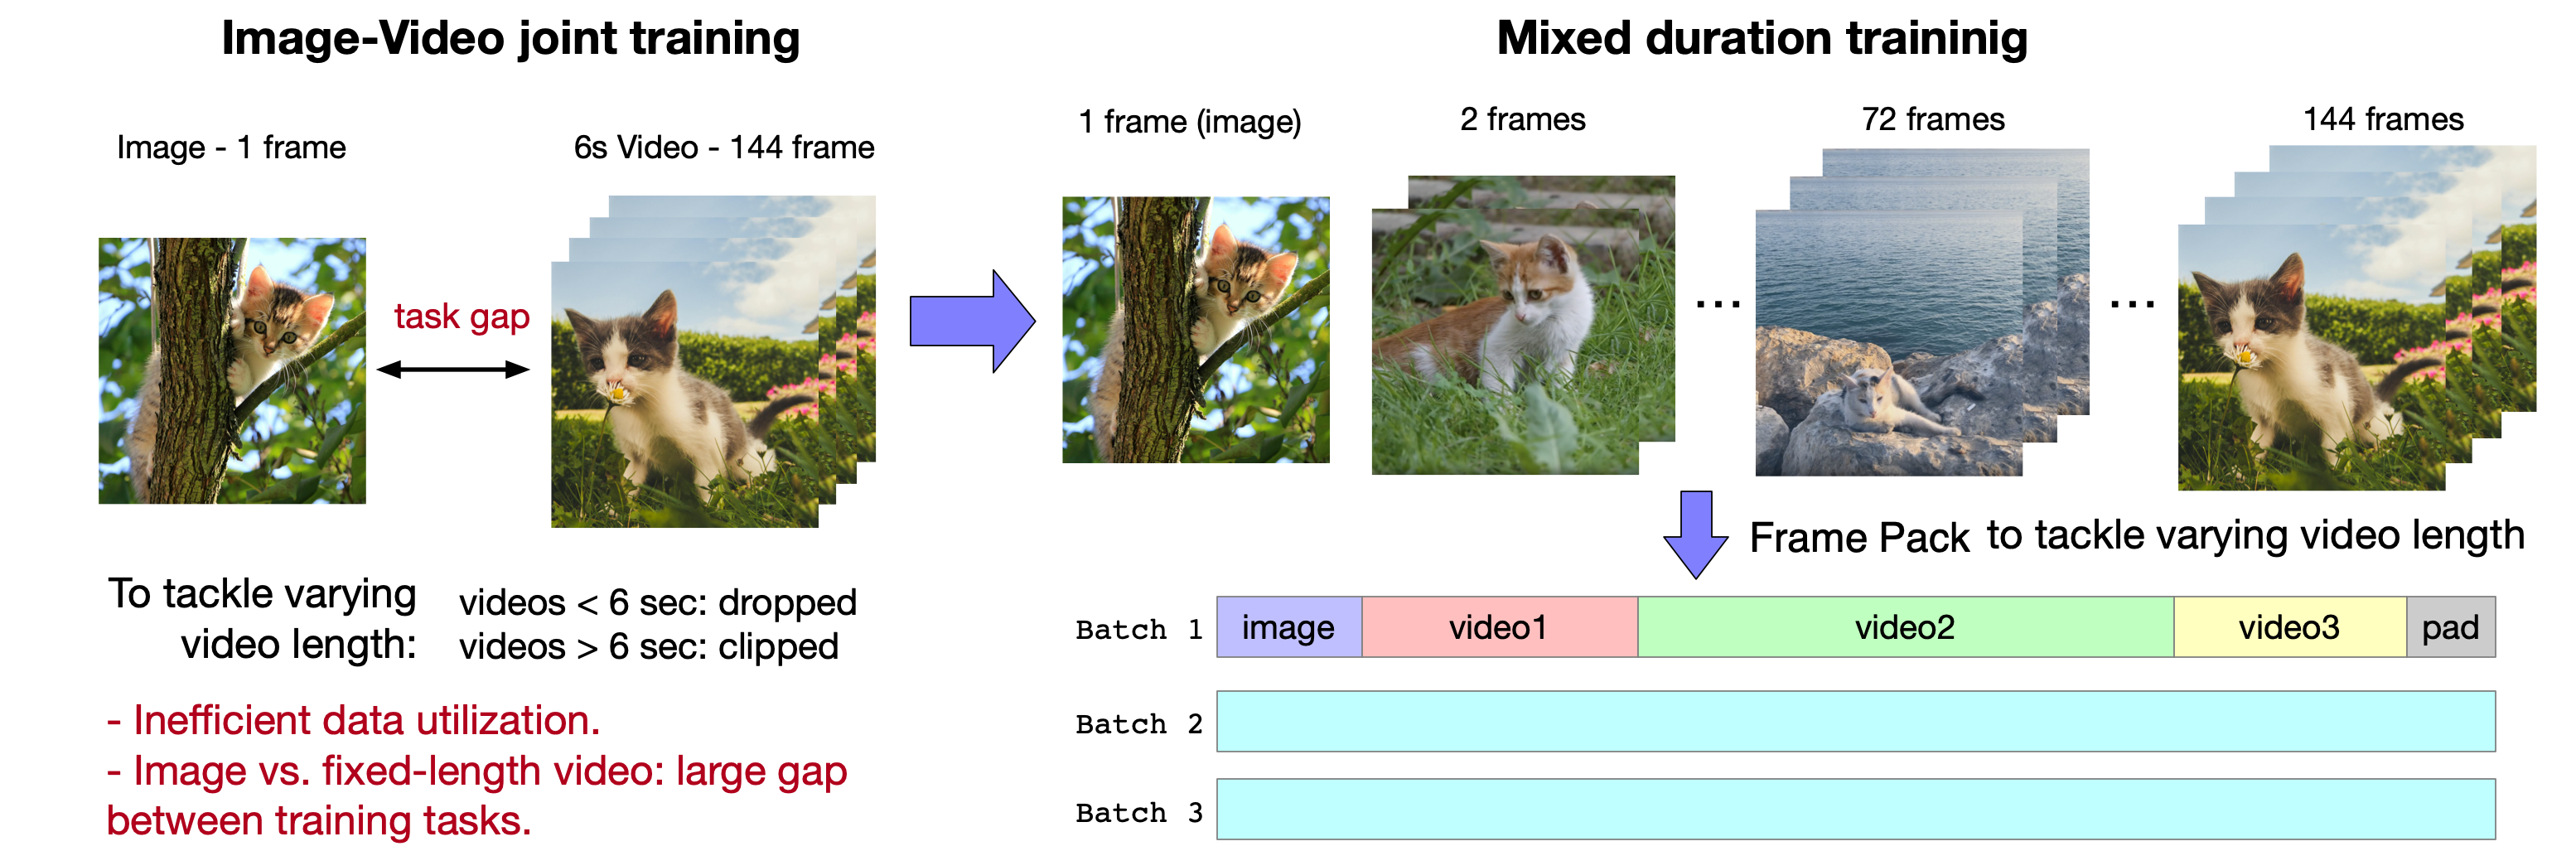
\includegraphics[width=\linewidth]{images/CogVideoX.png}
\end{center}
\caption{
The diagram of Mixed duration training and Frame Pack. To fully utilize the data and enhance the model's generalization capability, we train with videos of different durations within the same batch.}
\label{fig:framepack}
\end{figure}

\subsection{Setting}
We mixed images and videos during training, treating each image as a single-frame video. Additionally, we employed progressive training from the resolution perspective. For the diffusion setting, we adopt v-prediction~\citep{salimans2022progressive} and zero SNR~\citep{lin2024common}, following the noise schedule used in LDM~\citep{rombach2022high}.
During diffusion training for timestep sampling, we also employed an explicit uniform timestep sampling method, which benefits stable training. 

\subsection{Frame Pack}
Previous video model training methods often involved jointly training images and fixed frames videos. However, this approach led to two major problems: 1. There is a significant gap between the two input types using bidirectional attention, with images having 1 frame while videos having dozens of frames. We observed that models trained this way tend to diverge into two generative modes based on the token number and do not generalize well. 2. For training with a fixed duration, we need to discard short videos and truncate long videos, which prevents full utilization of the videos of varying frames.

To address these issues, we chose mixed-duration training, which means training videos of different lengths together. However, inconsistent data shapes within the batch make training difficult. Inspired by Patch'n Pack \citep{dehghani2024patch}, we place videos of different lengths into the same batch to ensure consistent shapes within each batch, a method we refer to as Frame Pack. 

\subsection{resolution prograssive training}
Our training pipeline is divided into three stages: low-resolution training, high-resolution training, and high-quality video fine-tuning. Similar to images, internet videos also include a significant amount of low-resolution videos. Prograssive training can effectively utilize various resolution videos. 
Moreover, training at low resolution initially can equip the model with coarse-grained modeling capabilities, followed by high-resolution training to enhance the model's ability to capture fine details. Compared to direct high-resolution training, staged training can reduce the overall training time.
\begin{figure}[h]
\begin{center}
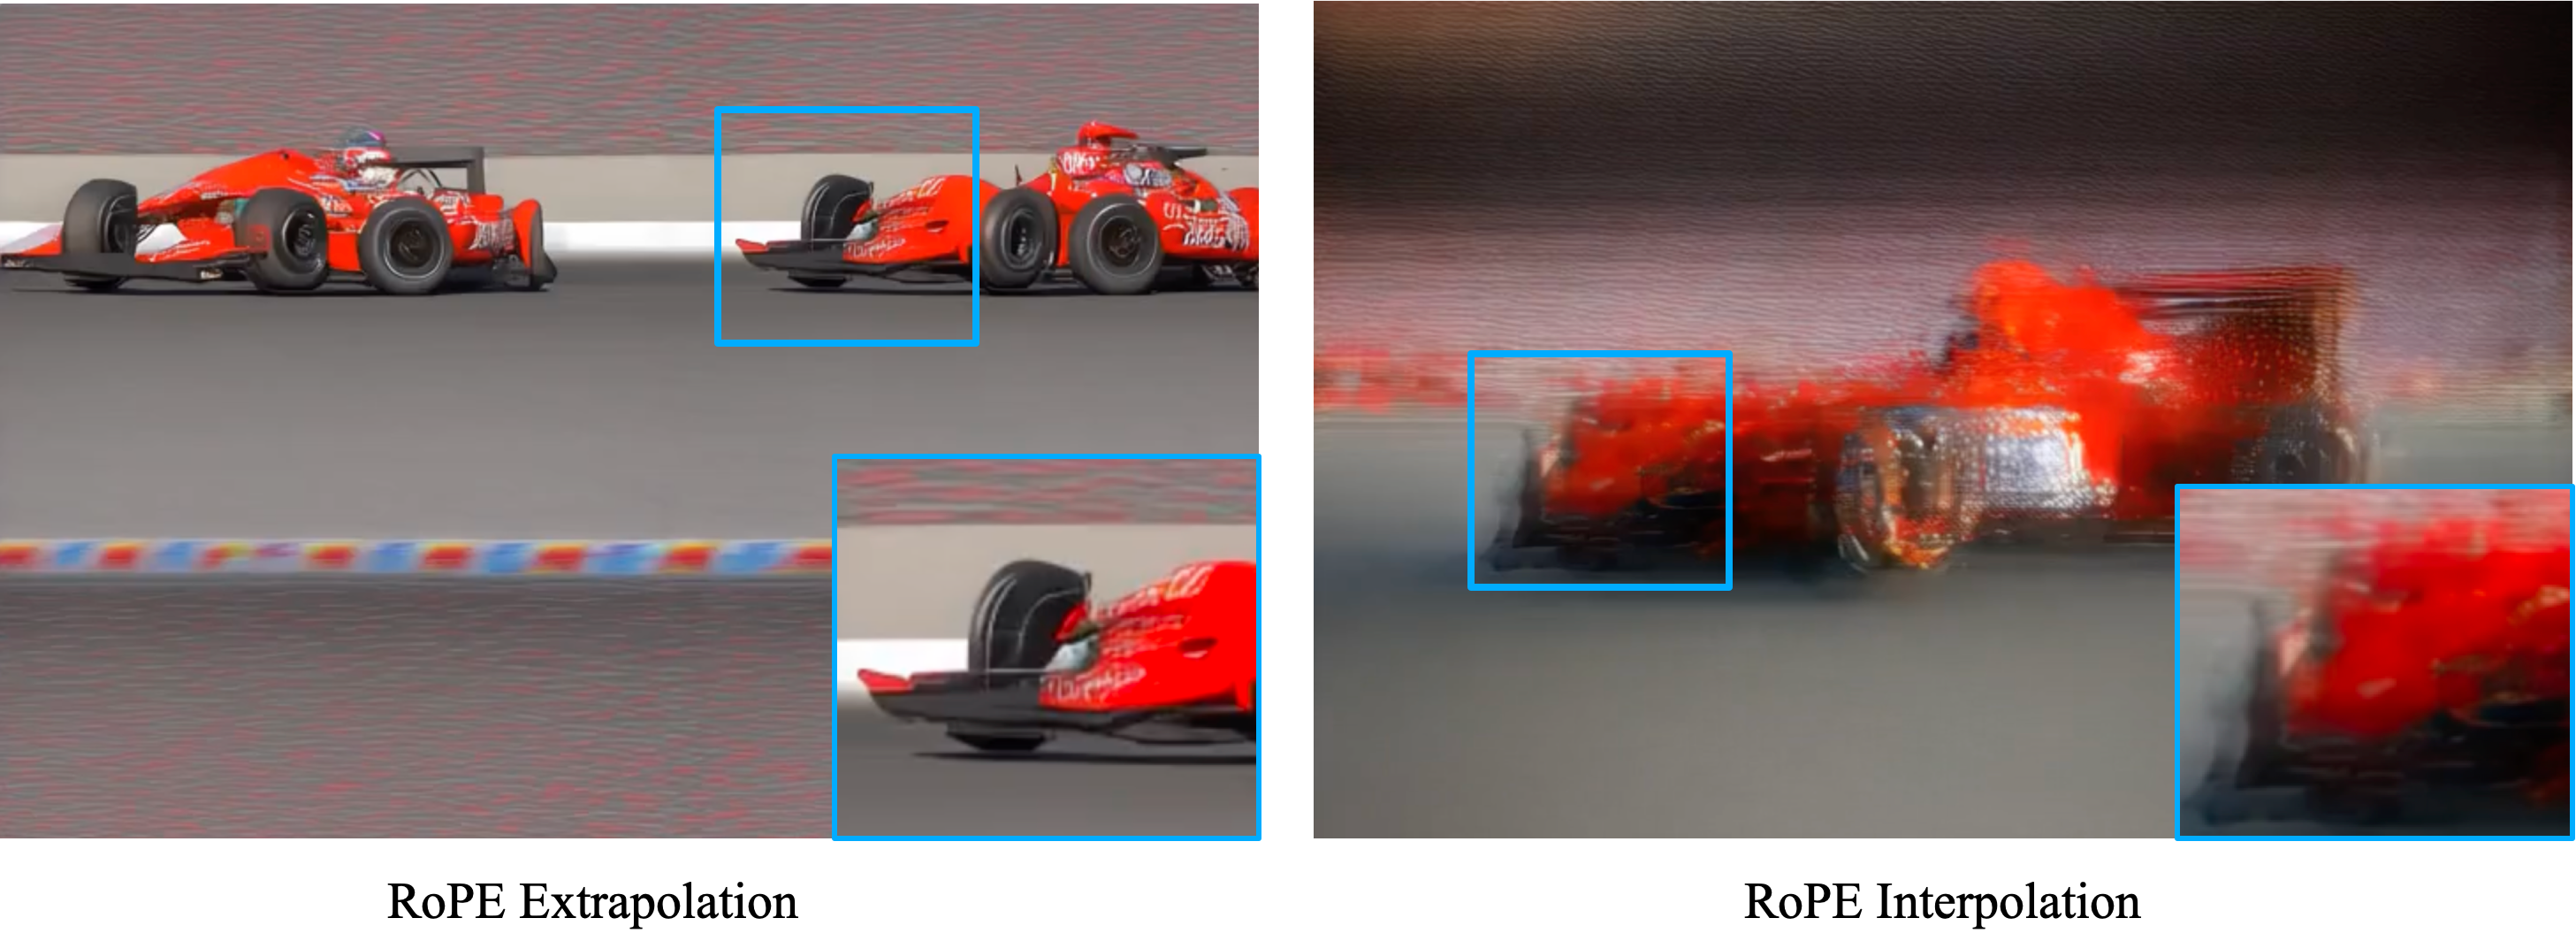
\includegraphics[width=0.9\linewidth]{images/ive.png}
\end{center}
\caption{We compared the initial generation states of extrapolation and interpolation when increasing resolution with RoPE encoding. Extrapolation tends to generate multiple small, clear, and repetitive images, while interpolation generates a blurry large image.}
\label{fig:ive}
\end{figure}

\paragraph{Extrapolation of position code}
When adapting low-resolution position encoding to high-resolution, we consider two different methods: interpolation and extrapolation. We show the effects of two methods in Figure~\ref{fig:ive}. Interpolation tens to preserve global information more effectively, whereas the extrapolation better retains local details. Given that RoPE is a relative position encoding, We chose the extrapolation to maintain the relative position between pixels. 

\paragraph{High-Quality fine-tuning}
Since the filtered pre-training data still contains a certain proportion of dirty data, such as subtitles, watermarks, and low-bitrate videos, we selected a subset of higher quality video data, accounting for 20\% of the total dataset, for fine-tuning in the final stage. This step effectively removed generated subtitles and watermarks and slightly improved the visual quality. However, we also observed a slight degradation in the model's semantic ability.


\subsection{Explicit Uniform Sampling}
~\citet{ho2020denoising} defines the training objective of diffusion as 
\begin{equation}~\label{eq:ddpm-loss}
    L_\mathrm{simple}(\theta) := \mathbf{E}_{t, x_0, \epsilon}{ \left\| \epsilon - \epsilon_\theta(\sqrt{\bar\alpha_t} x_0 + \sqrt{1-\bar\alpha_t}\epsilon, t) \right\|^2},
\end{equation}
where $t$ is uniformly distributed between 1 and T.
The common practice is for each rank in the data parallel group to uniformly sample a value between 1 and 
T. In theory, this is equivalent to Equation~\ref{eq:ddpm-loss}. However, in practice, the results obtained from such random sampling are often not sufficiently uniform, and since the magnitude of the diffusion loss is related to the timesteps, this can lead to significant fluctuations in the loss.
$Explicit\ Uniform\ Sampling$ is to divide the range from 1 to T into n intervals, where n is the number of ranks. Each rank then uniformly samples within its respective interval. This method ensures a more uniform distribution of timesteps. As shown in Figure~\ref{fig:a}, the loss curve from training with Explicit Uniform Sampling is noticeably more stable.

\section{Post-Training}
\label{section:finetuning}
We produce the aligned \llamathree~models by applying several rounds of post-training,\footnote{We use the term ``post-training'' to refer to any model training that happens outside of pre-training.} or aligning the model with human feedback~\citep{ouyang2022instructgpt,rafailov2024direct} on top of a pre-trained checkpoint. Each round of post-training involves supervised finetuning (SFT) followed by Direct Preference Optimization~\citep[DPO;][]{rafailov2024direct} on examples collected either via human annotations or generated synthetically. Our post-training modeling and data approaches are described in Sections~\ref{sec:finetuning_modeling} and ~\ref{sec:finetuning_data} respectively.
We further detail custom data curation strategies to improve the reasoning, coding, factuality, multilingual, tool use, long context, and precise instruction following in Section~\ref{sec:Capabilities}.

\begin{figure}[t]
    \centering
    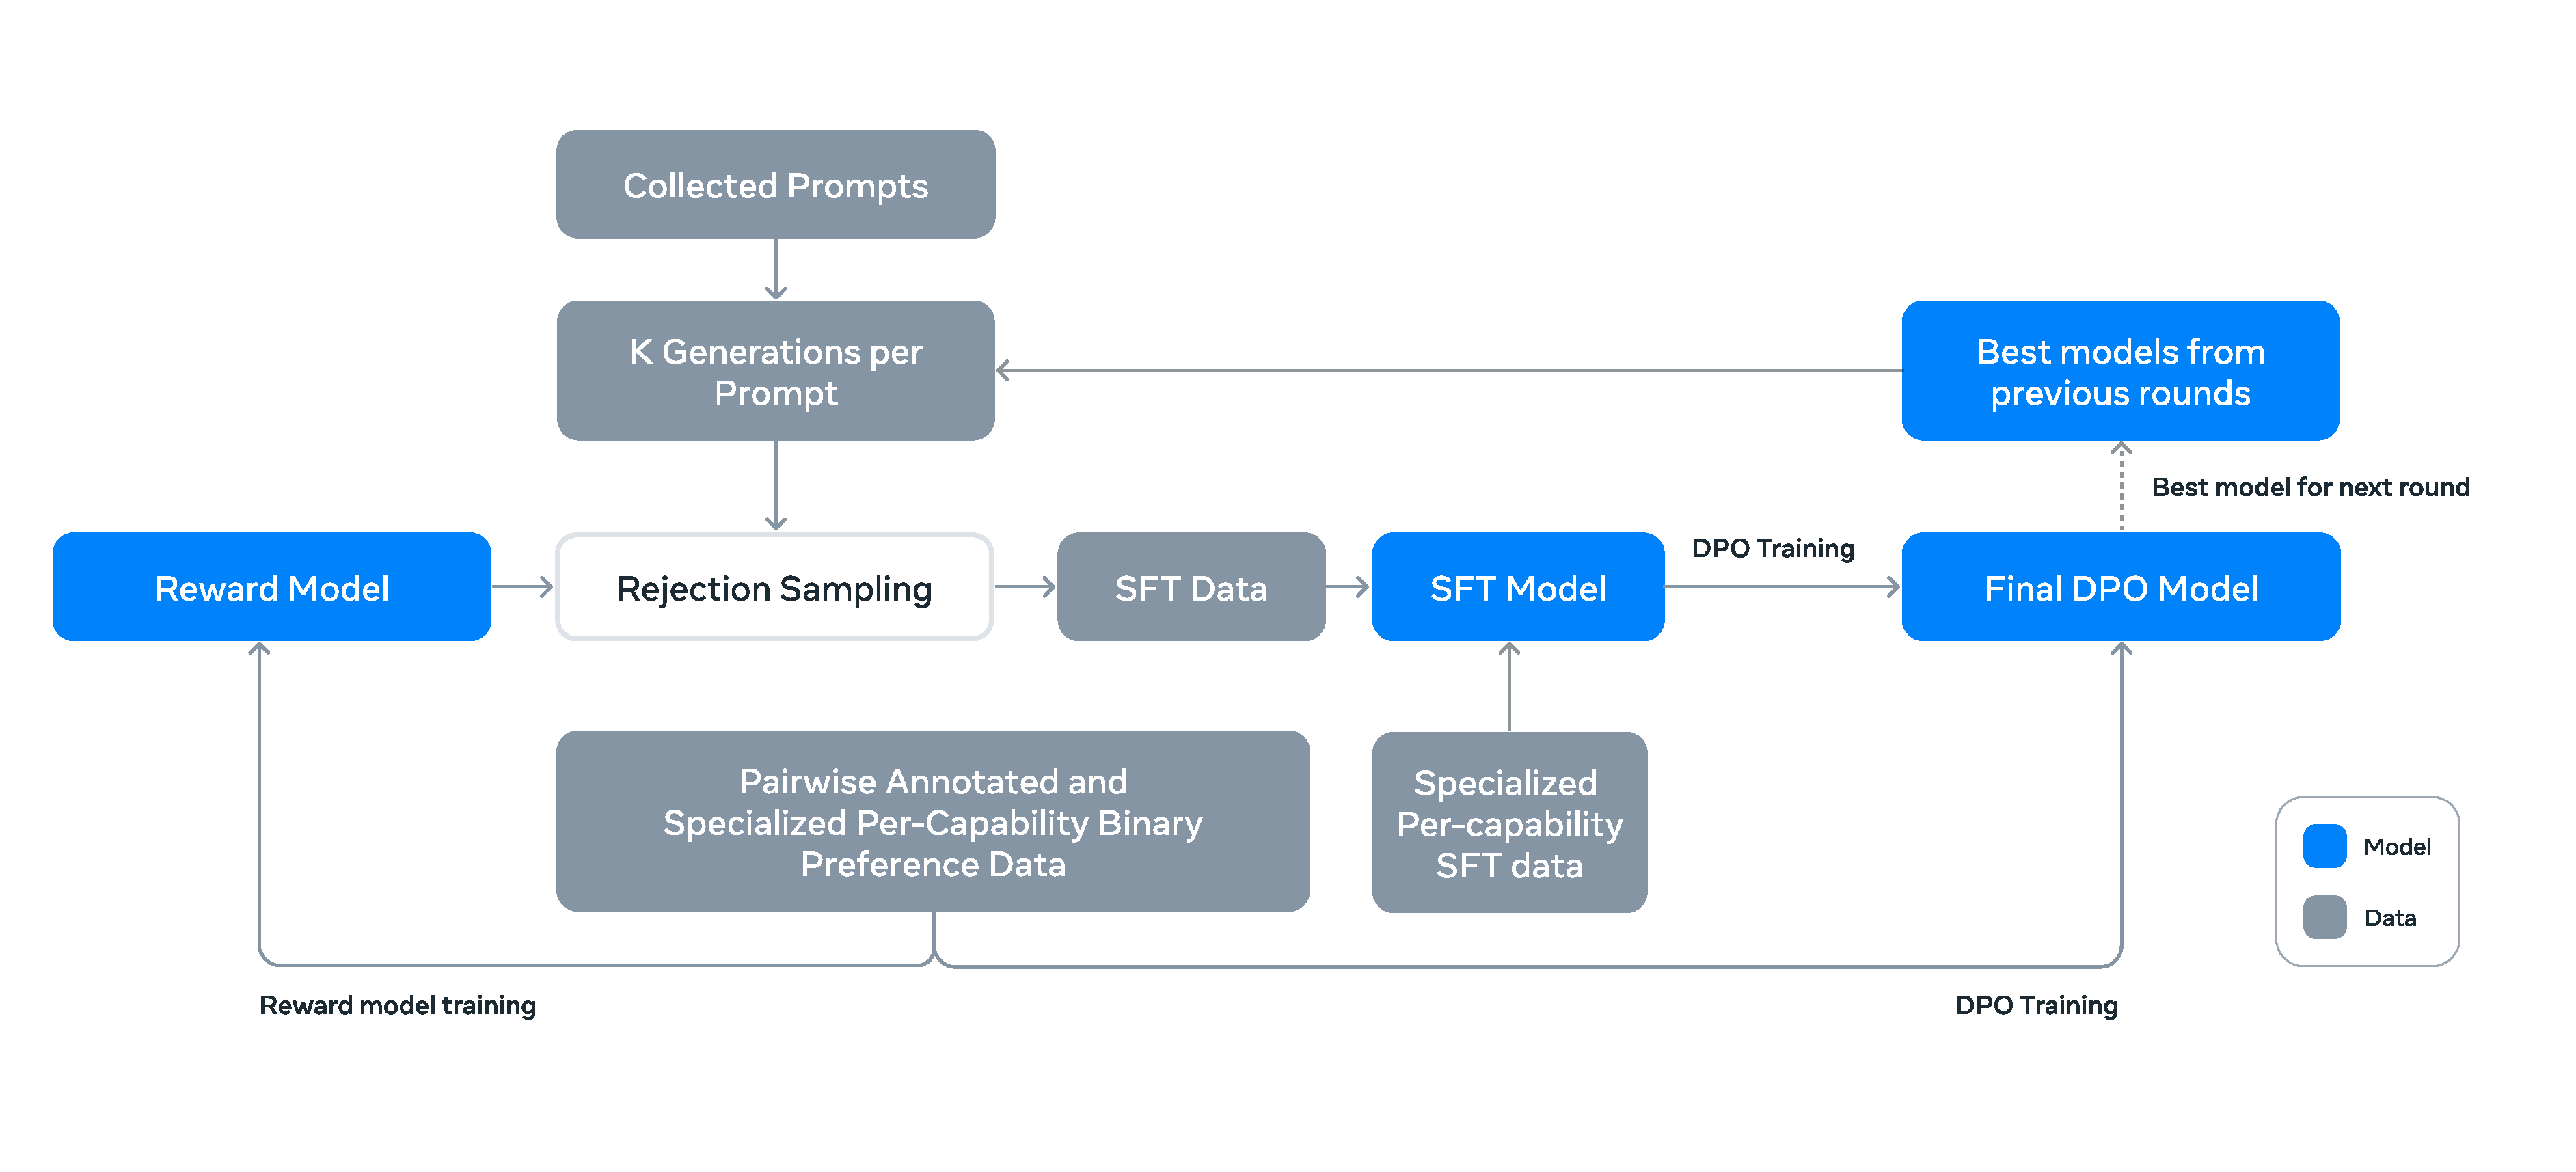
\includegraphics[width=\textwidth]{assets/posttraining_overview.pdf}
    \caption{\textbf{Illustration of the overall post-training approach for Llama 3.} Our post-training strategy involves rejection sampling, supervised finetuning, and direct preference optimization. See text for details.}
    \label{fig:posttraining_overview}
\end{figure}

\subsection{Modeling}
\label{sec:finetuning_modeling}
The backbone of our post-training strategy is a reward model and a language model. We first train a reward model on top of the pre-trained checkpoint using human-annotated preference data (see Section~\ref{subsubsec:rm}). We then finetune pre-trained checkpoints with supervised finetuning (SFT; see Section~\ref{subsubsec:sft}), and further align the checkpoints with Direct Preference Optimization (DPO; see Section~\ref{subsubsec:postdpo}).
This process is illustrated in Figure~\ref{fig:posttraining_overview}.
Unless otherwise noted, our modeling procedure applies to \llamathree~405B, and we refer to \llamathree~405B as \llamathree~for simplicity. 

\subsubsection{Chat Dialog Format}
\label{subsubsec:chat_format_content}

To tune LLMs for human-AI interaction, we need to define a chat dialog protocol for the model to understand human instructions and perform conversational tasks. Compared to its predecessor, \llamathree~has new capabilities such as tool use (Section~\ref{subsubsec:tool_use}) which may require generating multiple messages and sending them to different locations (e.g., user, \texttt{ipython}) within a single dialog turn. To support this, we design a new multi-message chat protocol which uses various special header and termination tokens. The header tokens are used to indicate the source and destination of each message in a conversation. Similarly, the termination tokens indicate when it is the time to alternate between human and AI to speak. 

\subsubsection{Reward Modeling}
\label{subsubsec:rm}

We train a reward model (RM) covering different capabilities on top of the pre-trained checkpoint. The training objective is the same as \llamatwo~except that we remove the margin term in the loss, as we observe diminishing improvements after data scaling. Following Llama 2, we use all of our preference data for reward modeling after filtering out samples with similar responses. In addition to standard preference pair of (chosen, rejected) response, annotations also create a third ``edited response'' for some prompts, where the chosen response from the pair is further edited for improvement (see Section~\ref{sec:rlhf_annotation_data}). Hence, each preference ranking sample has two or three responses with clear ranking (\emph{edited} > \emph{chosen} > \emph{rejected}). We concatenate the prompt and multiple responses into a single row during training with responses randomly shuffled. This is an approximation to the standard scenario of putting the responses in separate rows and computing the scores, but in our ablations, this approach improves training efficiency without a loss in accuracy. 


\subsubsection{Supervised Finetuning}
\label{subsubsec:sft}
The reward model is then used to perform rejection sampling on our human annotation prompts, the details of which are described in Section~\ref{sec:finetuning_data}. Together with this rejection-sampled data and other data sources (including synthetic data), we finetune the pre-trained language model using a standard cross entropy loss on the target tokens (while masking loss on prompt tokens).
More details about the data mix can be found in Section~\ref{sec:finetuning_data}.
We refer to this stage as \emph{supervised finetuning} \citep[SFT;][]{weifinetuned,sanh2022multitask,wang2022super}, even though many of the training targets are model-generated.
Our largest models are finetuned with a learning rate of $10^{-5}$ over the course of 8.5K to 9K steps. We found these hyperparameter settings to work well across different rounds and data mixes.

\subsubsection{Direct Preference Optimization}
\label{subsubsec:postdpo}

We further train our SFT models with Direct Preference Optimization \citep[DPO;][]{rafailov2024direct} for human preference alignment. For training, we primarily use the most recent batches of preference data collected using the best performing models from the previous alignment rounds. As a result, our training data conforms better to the distribution of the policy model that is being optimized in each round. We also explored on-policy algorithms such as PPO~\citep{schulman2017proximal}, but found that DPO required less compute for large-scale models and performed better, especially on instruction following benchmarks like IFEval~\citep{zhou2023instruction}.
For Llama~3, we use a learning rate of $10^{-5}$ and set the $\beta$ hyper-parameter to be 0.1. In addition, we apply the following algorithmic modifications to DPO:

\begin{itemize}
    \item \textbf{Masking out formatting tokens in DPO loss}: We mask out special formatting tokens including header and termination tokens (described in Section~\ref{subsubsec:chat_format_content}) from both chosen and rejected responses in the loss to stabilize DPO training. We observe that having these tokens contribute to the loss may lead to undesired model behaviors such as tail repetition or abruptly generating termination tokens. We hypothesize that this is due to the contrastive nature of the DPO loss -- the presence of common tokens in both chosen and rejected responses leads to a conflicting learning objective as the model needs to increase and reduce the likelihood of these tokens simultaneously. 
    \item \textbf{Regularization with NLL loss}: We add an additional negative log-likelihood (NLL)  loss term with a scaling coefficient of $0.2$ on the chosen sequences, similar to~\citet{pang2024iterative}. This helps further stabilize DPO training by maintaining desired formatting for generation and preventing the decrease of log probability of chosen responses~\citep{pang2024iterative, pal2024smaug}. 
\end{itemize}

\subsubsection{Model Averaging}

Finally, we average models obtained from experiments using various versions of data or hyperparameters at each RM, SFT, or DPO stage~\citep{izmailov2019averagingweightsleadswider,wortsman2022modelsoupsaveragingweights, li2022branchtrainmergeembarrassinglyparalleltraining}. 

\subsubsection{Iterative Rounds}

Following Llama 2, we apply the above methods in six rounds. In each cycle, we collect new preference annotations and SFT data, sampling synthetic data from the latest models. 

\subsection{Post-training Data}
\label{sec:finetuning_data}

The post-training data composition plays a critical role in the usefulness and behavior of language models. In this section, we discuss our human annotation procedures and preference data collection (Section~\ref{sec:rlhf_annotation_data}), the composition of our SFT data (Section~\ref{subsubsec:sft_data}), and methods for data quality control and cleaning (Section~\ref{subsubsec:data_clean}).


\subsubsection{Preference Data} 
\label{sec:rlhf_annotation_data}

Our preference data annotation process is similar to Llama~2. We deploy multiple models for annotation after each round and sample two responses from two different models for each user prompt. These models can be trained with different data mixes and alignment recipes, allowing for different capability strength (\emph{e.g.}, code expertise) and increased data diversity. We ask annotators to rate the strength of their preference by categorizing it into one of four levels, based on how much more they prefer the chosen response over the rejected one: significantly better, better, slightly better, or marginally better. We also incorporate an editing step after preference ranking to encourage annotators to further improve the preferred response. Annotators edit the chosen response directly or prompt the model with feedback to refine its own response. Consequently, a portion of our preference data has three responses ranked (\emph{edited} > \emph{chosen} > \emph{rejected}).

In Table~\ref{tab:pref_data}, we report the statistics of preference annotations that we use for \llamathree training. 
General English covers multiple subcategories such as knowledge-based question and answering or precise instruction-following, which fall outside the scope of specific capabilities. Compared to Llama~2, we observe an increase in the average length of prompt and response, suggesting that we train \llamathree on more complex tasks. In addition, we implement a quality analysis and human evaluation process to rigorously assess the data collected, allowing us to refine our prompts and provide systematic, actionable feedback to annotators. For example, as \llamathree improves after each round, we increase prompt complexity accordingly to target areas where the model lags.

In each round of post-training, we use all the preference data that is available at the time for reward modeling, while only using the latest batches from various capabilities for DPO training. For both reward modeling and DPO, we use samples that are labeled as the chosen response being significantly better or better than the rejected counterpart for training and discard samples with similar responses.

\begin{table}[t]
  \centering
  \setlength{\tabcolsep}{4pt}
   {
  \begin{tabular}{@{}l@{\hspace*{0mm}}rrrrr@{}}
    \toprule
      & \textbf{\% of} & \textbf{Avg. \# turns} & \textbf{Avg. \# tokens} & \textbf{Avg. \# tokens} & \textbf{Avg. \# tokens} \\
     \textbf{Dataset} & \textbf{comparisons} &\textbf{per dialog} & \textbf{per example} &\textbf{in prompt} & \textbf{in response} \\
    \midrule
    General English & 81.99\% & 4.1 & 1,000.4 & 36.4 & 271.2 \\
    Coding & 6.93\% & 3.2 & 1,621.0 & 113.8 & 462.9 \\
    Multilingual & 5.19\% & 1.8 & 1,299.4 & 77.1 & 420.9 \\ 
    Reasoning and tools & 5.89\% & 1.6 & 707.7 & 46.6 & 129.9 \\
    \midrule
    Total & 100\% & 3.8 & 1,041.6 & 44.5 & 284.0 \\
    \bottomrule
  \end{tabular}}
  \vspace{0.3cm}
  \caption{\textbf{Statistics of human preference data.} We list statistics of the internally collected human preference data used for \llamathree alignment. We ask annotators to perform multi-turn dialogues with the models and make comparisons among responses at each turn. In post-processing, we split each dialogue to multiple examples at a turn level. Each example consists of a prompt (including previous dialog if available) and a response (e.g., chosen or rejected response).}
  \label{tab:pref_data}
\end{table}



\subsubsection{SFT Data}
\label{subsubsec:sft_data} 

Our finetuning data is largely comprised of the following sources:

\begin{itemize}
    \item Prompts from our human annotation collection with rejection-sampled responses.
    \item Synthetic data targeting specific capabilities (see Section~\ref{sec:Capabilities} for more details).
    \item Small amounts of human-curated data (see Section~\ref{sec:Capabilities} for more details).
\end{itemize}

As our post-training rounds progress, we develop stronger \llamathree variants that we use to collect larger datasets that cover a wide range of complex capabilities. In this section, we discuss the details for the rejection-sampling procedure and overall composition of our final SFT datamix.


\textbf{Rejection sampling.}
During rejection sampling (RS), for each prompt collected during human annotation (Section~\ref{sec:rlhf_annotation_data}) we sample $K$ (typically between 10 and 30) outputs from the latest chat model policy (usually the best performing checkpoint from the previous post-training iteration, or the best performing checkpoint for a particular capability) and use our reward model to select the best candidate, consistent with~\citet{constitutional-ai-bai}. 
In later rounds of post-training, we introduce system prompts to steer RS responses to conform with desirable tone, style, or formatting, which might be different for different capabilities. 

To increase the efficiency of rejection sampling, we adopt PagedAttention~\citep{kwon2023efficient}.
PagedAttention enhances memory efficiency through dynamic key-value cache allocation. 
It supports arbitrary output lengths by dynamically scheduling requests based on the current cache capacity.
Unfortunately, this carries the risk of swap-out when running out of memory. 
To eliminate such swap overhead, we define a maximum output length and perform a request only if sufficient memory is available to fit an output with that length.
PagedAttention also enables us to share the key-value cache pages for a prompt across all corresponding outputs.
Together, this leads to a throughput improvement of over $2 \times$ during rejection sampling.


\textbf{Overall data composition.} Table~\ref{tab:sft_data} shows data statistics for each broad category of our ``helpfulness'' mix. 
While SFT and preference data contain overlapping domains, they are curated differently, yielding distinct count statistics. In Section~\ref{subsubsec:data_clean} we describe techniques for categorizing topic, complexity, and quality of our data samples. In each round of post-training, we adjust our overall data mix carefully across these axes to tune performance across a wide range of benchmarks. Our final data mix epochs multiple times on some high quality sources and downsamples others.


\begin{table}[t]
  \centering
  \setlength{\tabcolsep}{4pt}
   {
  \begin{tabular}{@{}l@{\hspace*{0mm}}rrrrr@{}}
    \toprule
      & & & & \textbf{Avg. \# tokens} & \textbf{Avg. \# tokens} \\
     \textbf{Dataset} & \textbf{\% of examples} & \textbf{Avg. \# turns} & \textbf{Avg. \# tokens} & \textbf{in context} & \textbf{in final response} \\
   \midrule
   General English & 52.66\% & 6.3 & 974.0 & 656.7 & 317.1\\
    Code & 14.89\% & 2.7 & 753.3 &  378.8  & 374.5 \\
    Multilingual & 3.01\% & 2.7 & 520.5 & 230.8 & 289.7 \\
    Exam-like & 8.14\% & 2.3 & 297.8 &  124.4 & 173.4 \\
    Reasoning and tools & 21.19\% & 3.1  & 661.6 & 359.8 & 301.9 \\
    Long context & 0.11\% & 6.7 & 38,135.6 & 37,395.2 & 740.5 \\
    \midrule
    Total & $100\%$ & 4.7 & 846.1 & 535.7 & 310.4 \\
    \bottomrule
  \end{tabular}}
  \vspace{0.3cm}
  \caption{\textbf{Statistics of SFT data.} We list internally collected SFT data used for \llamathree alignment. Each SFT example consists of a context (i.e., all conversation turns except the last one) and a final response.}
  \label{tab:sft_data}
\end{table}



\subsubsection{Data Processing and Quality Control}
\label{subsubsec:data_clean} 

Given that most of our training data is \emph{model-generated}, it requires careful cleaning and quality control. 

\textbf{Data cleaning.} In the early rounds, we observed a number of undesirable patterns common in our data, such as excessive use of emojis or exclamation points. Therefore, we implement a series of rule-based data removal and modification strategies to filter or clean problematic data. For example, to mitigate overly-apologetic tonal issues, we identify overused phrases (such as ``I'm sorry'' or ``I apologize'') and carefully balance the proportion of such samples in our dataset. 


\textbf{Data pruning.} 
We also apply a collection of model-based techniques to remove low-quality training samples and improve overall model performance:

\begin{itemize}
    \item \textbf{Topic classification:} We first finetune \llamathree 8B into a topic classifier, and perform inference over all data to classify it into both coarsely-grained buckets (``mathematical reasoning'') and fine-grained buckets (``geometry and trigonometry''). 

    \item \textbf{Quality scoring:} We use both reward model and Llama-based signals to obtain a quality score for each sample. 
    For an RM-based score, we consider data that is in the top quartile of RM scores as high quality.
    For a Llama-based score, we prompt \llamathree~checkpoint to rate each sample on a three-point scale for general English data (accuracy, instruction following, and tone/presentation) and a two-point scale for coding data (bug identification and user intention), and consider samples that obtain the maximum score as high quality. 
    The RM and Llama-based scores have high disagreement rates, and we find that combining these signals yield the best recall on our internal test set. Ultimately, we select examples that are marked as high quality by the RM \emph{or} the Llama-based filter. 

    \item \textbf{Difficulty scoring:} 
    Because we are also interested in prioritizing examples that are more complex for the model, we score data using two measures of difficulty: Instag \citep{lu2023instag} and Llama-based scoring. For Instag, we prompt \llamathree 70B to perform intention tagging of SFT prompts, where more intentions implies more complexity. We also prompt \llamathree to measure the difficulty \citep{liu2024makesgooddataalignment} of dialogs on a three-point scale. 

    \item \textbf{Semantic deduplication:} Finally, we perform semantic deduplication \citep{abbas2023semdedup, liu2024makesgooddataalignment}. We first cluster complete dialogs using RoBERTa \citep{liu_ott_roberta} and within each cluster sort them by quality score $\times$ difficulty score. We then do greedy selection by iterating through all sorted examples, and only keeping the ones that have maximum cosine similarity less than a threshold to the examples seen so far in the cluster.

\end{itemize}


\subsection{Capabilities}
\label{sec:Capabilities}

We highlight special efforts to improve performance for specific capabilities such as code (Section~\ref{subsubsec:code}), multilinguality (Section~\ref{subsubsec:multilingual}), math and reasoning (Section~\ref{subsubsec:reasoning}), long context (Section~\ref{subsubsec:long_context}), tool use (Section~\ref{subsubsec:tool_use}), factuality (Section~\ref{subsubsec:factuality}), and steerability (Section~\ref{subsubsec:steerability}).  

\subsubsection{Code}
\label{subsubsec:code}

LLMs for code have received significant attention since the release of Copilot and Codex~\citep{chen2021evaluating}. 
Developers are now widely using these models to generate code snippets, debug, automate tasks, and improve code quality.
For \llamathree, we target improving and evaluating code generation, documentation, debugging, and review capabilities for the following high priority programming languages: Python, Java, Javascript, C/C++, Typescript, Rust, PHP, HTML/CSS, SQL, bash/shell. 
Here, we present our work on improving these coding capabilities via training a code expert, generating synthetic data for SFT, improving formatting with system prompt steering, and creating quality filters to remove bad samples from our training data.

\textbf{Expert training.} We train a \textbf{code expert} which we use to collect high quality human annotations for code throughout subsequent rounds of post-training. This is accomplished by branching the main pre-training run and continuing pre-training on a 1T token mix of mostly (>85\%) code data. Continued pre-training on domain-specific data has been shown to be effective for improving performance in a specific domain~\citep{gururangan2024dontstoppretraining}. We follow a recipe similar to that of CodeLlama \citep{codellama}. For the last several thousand steps of training we perform {long-context finetuning} (LCFT) to extend the expert's context length to 16K tokens on a high quality mix of repo-level code data. Finally, we follow the similar post-training modeling recipes described in Section~\ref{sec:finetuning_modeling} to align this model, except with SFT and DPO data mixes primarily targeting code.  This model is also used for rejection sampling (Section~\ref{subsubsec:sft_data}) for coding prompts.

\textbf{Synthetic data generation.}
During development, we identified key issues in code generation, including difficulty in following instructions, code syntax errors, incorrect code generation, and difficulty in fixing bugs. While intensive human annotation could theoretically resolve these issues, synthetic data generation offers a complementary approach at a lower cost and higher scale, unconstrained by the expertise level of annotators. As such, we use \llamathree and the code expert to generate a large quantity of synthetic SFT dialogs. 

We describe three high-level approaches for generating synthetic code data. In total, we generate over $2.7$M synthetic examples which were used during SFT.

\begin{enumerate}
    \item{\textbf{Synthetic data generation: execution feedback.}} The 8B and 70B models show significant performance improvements when trained on data generated by a larger, more competent model. However, our initial experiments revealed that training \llamathree 405B on its own generated data is not helpful (and can even degrade performance). To address this limitation, we introduced execution feedback as a source of truth, enabling the model to learn from its mistakes and stay on track. %
    In particular, we generate large dataset of approximately one million synthetic coding dialogues using the following process:


    \begin{itemize}
        \item \textbf{Problem description generation:}
        First, we generate a large collection of programming problem descriptions that span a diverse range of topics, including those in the long tail distribution. To achieve this diversity, we sample random code snippets from various sources and prompt the model to generate programming problems inspired by these examples. This allowed us to tap into a wide range of topics and create a comprehensive set of problem descriptions~\citep{wei2024magicoderempoweringcodegeneration}.
        
        
        \item \textbf{Solution generation:} Then, we prompt \llamathree to solve each problem in a given programming language. We observe that adding general rules of good programming to the prompt improves the generated solution quality. Also, we find it is helpful to require the model to explain its thought process in comments.
        
        \item \textbf{Correctness analysis:}
        After generating a solution, it is crucial to recognize that its correctness is not guaranteed, and including incorrect solutions in the finetuning dataset could harm the model's quality. While we do not ensure complete correctness, we develop methods to approximate it. To achieve this, we extract the source code from the generated solution and applied a combination of static and dynamic analysis techniques to test its correctness, including:
        
        \begin{itemize}{
        \item \textbf{Static analysis}: We run all generated code through a parser and a linter to ensure syntactic correctness, catching errors such as syntax errors, use of uninitialized variables or non-imported functions, code style issues, typing errors, and others.
        \item \textbf{Unit test generation and execution}: For each problem and solution, we prompt the model to generate unit tests, executed in a containerized environment together with the solution, catching run-time execution errors and some semantic errors.
        }\end{itemize}
        
        \item \textbf{Error feedback and iterative self-correction:}
        When a solution fails at any step, we prompt the model to revise it. The prompt included the original problem description, the faulty solution, and feedback from the parser/linter/tester (stdout, stderr/ and return code). %
        After a unit test execution failure, the model could either fix the code to pass the existing tests or modify its unit tests to accommodate the generated code.
        Only dialogs that pass all checks are included in the final dataset, used for supervised finetuning (SFT). Notably, we observed that about 20\% of solutions were initially incorrect but self-corrected, indicating that the model learned from the execution feedback and improved its performance.
        
        \item \textbf{Fine-tuning and iterative improvement:} The finetuning process is conducted over multiple rounds, with each round building on the previous one. After each round, the model is improved, generating higher-quality synthetic data for the next round. This iterative process allows for progressive refinement and enhancement of the model's performance.
    \end{itemize}

    \item{\textbf{Synthetic data generation: programming language translation.}} We observe a performance gap between major programming languages (\emph{e.g.}, Python/C++) and less common ones (\emph{e.g.}, Typescript/PHP). This is not surprising as we have less training data for less common programming languages. To mitigate this, we supplement our existing data by \emph{translating} data from common programming languages to less common languages (similar to \cite{chen2023breakinglanguagebarriersmultilingual} in the context of reasoning). This is achieved by prompting \llamathree and ensuring quality via syntax parsing, compilation, and execution. Figure~\ref{fig:code_translation_example} demonstrates an example of synthetic PHP code translated from Python. This improves performance significantly for less common languages as measured by the MultiPL-E \citep{cassano2022multiple} benchmark. 
    
    \begin{figure}
    \centering
    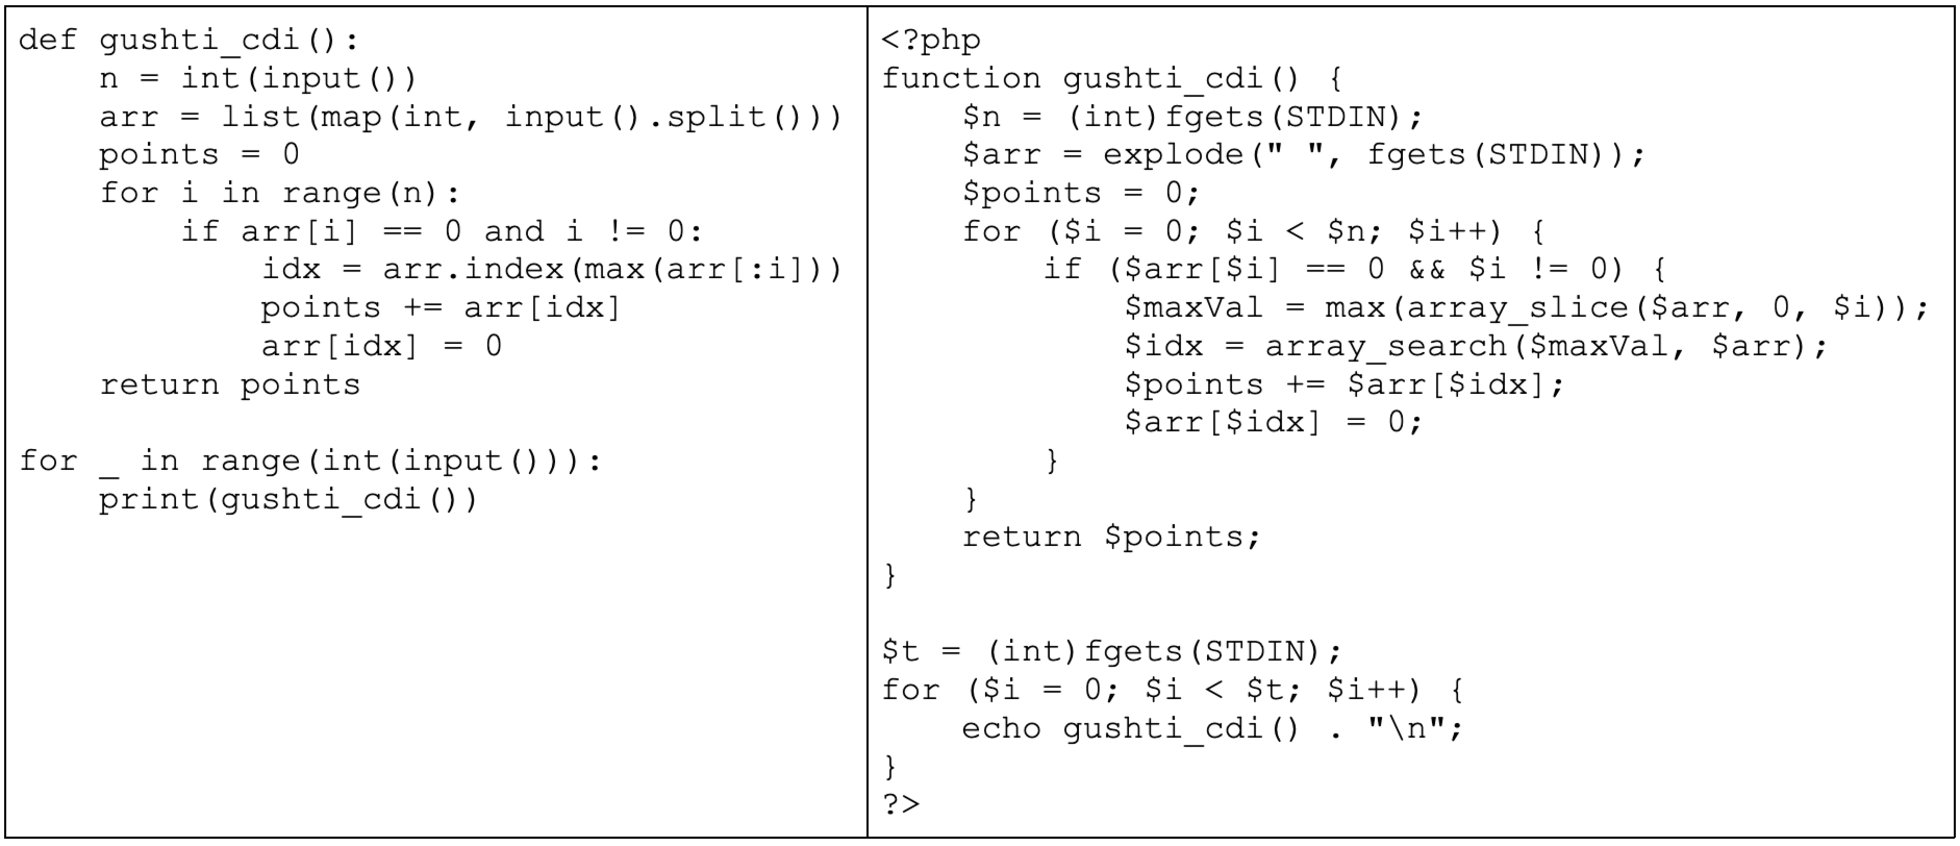
\includegraphics[width=0.75\linewidth]{posttraining/assets/code_translation_example.pdf}
    \caption{\label{fig:code_translation_example} \textbf{Code translation example.} We display an example of using \llamathree to translate Python code (left) to PHP code (right) to augment our SFT dataset with a wider range of programming languages.}
    \end{figure}


    \item{\textbf{Synthetic data generation: backtranslation.}} To improve certain coding capabilities (e.g., documentation, explanations) where execution feedback is less informative for determining quality, we employ an alternative multi-step approach. Using this procedure, we generated approximately 1.2M synthetic dialogs related to code explanation, generation, documentation, and debugging. Beginning with code snippets from a variety of languages in our pre-training data:
    \begin{itemize}
        \item \textbf{Generate:} We prompt \llamathree~to generate data that represents our target capability (e.g., we add comments and docstrings for the code snippet, or we ask the model to explain a piece of code).
        \item \textbf{Backtranslate:} We then prompt the model to ``backtranslate'' the synthetically generated data to the original code (e.g., we prompt the model to generate code only from its documentation, or we ask the model to generate code only from its explanation).
        \item \textbf{Filter:} Using the original code as a reference, we prompt the \llamathree to determine the quality of the output (e.g., we ask the model how faithful the backtranslated code is to the original). We then use the generated examples that have the highest self-verification scores in SFT. 
    \end{itemize}

\end{enumerate}


\textbf{System prompt steering during rejection sampling.} 
During the rejection sampling process, we used code specific system prompts to improve 
code readability, documentation, thoroughness, and specificity. Recall, from Section~\ref{tab:sft_data} this data is used to finetune the language model.  Figure \ref{fig:code_system_prompt_example} shows an example of how the system prompt helps improve the generated code quality --- it  adds necessary comments, uses more informative variable names, saves memory, etc.

\begin{figure}
\centering
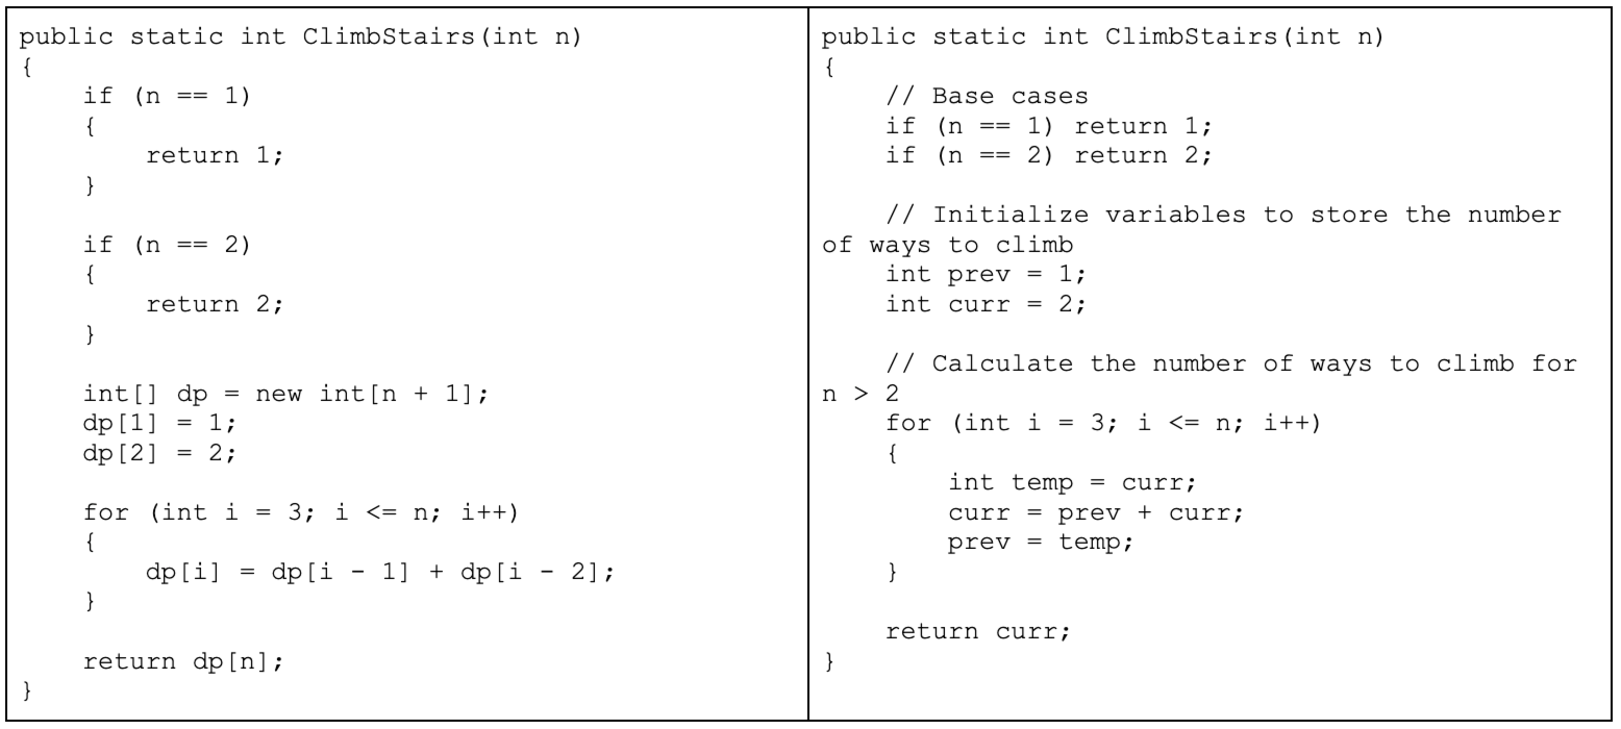
\includegraphics[width=0.75\linewidth]{posttraining/assets/code_system_prompt_example.pdf}
\caption{\label{fig:code_system_prompt_example} \textbf{Improving generated code quality with system prompts.} \emph{Left:} without system prompt \emph{Right:} with system prompt.}
\end{figure}

\textbf{Filtering training data with execution and model-as-judge signals.} 
As described in Section~\ref{subsubsec:data_clean}, we occasionally encounter quality issues in our rejection-sampled data, such as code blocks containing bugs. Detecting these issues in our rejection-sampled data is not as straightforward as it is for our \emph{synthetic code data}, as the rejection-sampled responses typically contain a mix of natural language and code for which the code may not always be expected to be executable. (For example, user prompts may explicitly ask for pseudo-code or edits to only a very small snippet of an executable program.) To address this, we utilize the ``model-as-judge'' approach, where earlier versions of \llamathree assess and assign a binary (0/1) score based on two criteria: code correctness and code style. We retain only those samples that achieve a perfect score of 2. Initially, this stringent filtering led to a regression in downstream benchmark performance, primarily because it disproportionately removed examples with challenging prompts. To counteract this, we strategically revise the responses of some coding data categorized as most challenging until they met the Llama-based ``model-as-judge'' criteria. By refining these challenging problems, the coding data achieves a balance between quality and difficulty, resulting in optimal downstream performance.

\subsubsection{Multilinguality}
\label{subsubsec:multilingual}
We describe how we improve Llama 3's multilingual capabilities, including training an expert specialized on substantially more multilingual data, sourcing and generating high quality multilingual instruction tuning data for German, French, Italian, Portuguese, Hindi, Spanish, and Thai, and tackling specific challenges of multilingual language steering to enhance the overall performance of our model. 

\textbf{Expert training.} Our \llamathree pre-training data mix contains significantly more English tokens than non-English tokens. To collect higher quality human annotations in non-English languages, we train a \textbf{multilingual expert} by branching off the pre-training run and continuing to pre-train on a data mix that  consists of $90$\% multilingual tokens. We then perform post-training on this expert following Section~\ref{sec:finetuning_modeling}. This expert model is then used to collect higher quality annotations in non-English languages until pre-training was fully complete.

\textbf{Multilingual data collection.} Our multilingual SFT data is derived primarily from sources described below. The overall distribution is 2.4\% human annotations, 44.2\% data from other NLP tasks, 18.8\% rejection sampled data, and 34.6\% translated reasoning data.
\begin{itemize}
        \item \textbf{Human annotations}: We collect high-quality, manually annotated data from linguists and native speakers. These annotations mostly consist of open-ended prompts that represent real world use cases. %

        \item \textbf{Data from other NLP tasks}: To further augment, we use multilingual training data from other tasks and rewrite into dialog format. For example, we use data from exams-qa~\citep{hardalov-etal-2020-exams} and Conic10k~\citep{wu2023conic10kchallengingmathproblem}. To improve language alignment, we also use parallel texts from GlobalVoices~\citep{PROKOPIDIS16.778} and Wikimedia~\citep{Tiedemann2012ParallelDT}. We use LID based filtering and Blaser2.0~\citep{seamlessm4t2023} to remove low quality data. For parallel text data, instead of using the bitext pairs directly, we apply a multilingual template inspired by~\citet{weifinetuned} to better simulate real-life conversations in translation and language learning scenarios.
     
        \item \textbf{Rejection sampled data}: We apply rejection sampling on our human annotated prompts to generate high-quality samples for finetuning, with few modifications compared to the process for English data: 
            \begin{itemize} 
                \item \textbf{Generation}: 
                We explored randomly choosing the temperature hyperparameter from the range $0.2-1$ for diverse generations in early rounds of post-training. %
                With high temperature, responses for multilingual prompts can get creative and inspiring, but are also susceptible to unnecessary or unnatural code-switching. In the final round of post-training, we use a constant value of 0.6 to balance the trade-off. Additionally, we used specialized system prompts to improve response format, structure and general readability. 
                \item \textbf{Selection}: Prior to reward model based selection, we implement multilingual-specific checks to ensure high language-match rate between the prompt and response (e.g., a romanized Hindi prompt should not expect a response in Hindi Devanagari script). %
            \end{itemize}
        \item \textbf{Translated data}: We try to avoid using machine-translated data to finetune the model in order to prevent translationese~\citep{bizzoni-etal-2020-human,muennighoff2023crosslingual} or possible name bias~\citep{wang-etal-2022-measuring}, gender bias \citep{10.1162/tacl_a_00401}, or cultural bias~\citep{Ji_Ji_Bouillon_Seligman_2023}. Moreover, we aim to prevent the model from being exposed only to tasks that are rooted in English cultural context, which may not be representative of the linguistic and cultural diversity we aim to capture. We made one exception to this and translated our synthetic quantitative reasoning data (see Section~\ref{subsubsec:reasoning} for details) to improve performance in quantitative reasoning in non-English languages.
        Due to the simple nature of the language in these math problems, the translated samples were found to have little to no quality issues. We observed strong gains on MGSM~\citep{shi2022languagemodelsmultilingualchainofthought} from adding this translated data. 
\end{itemize}

\subsubsection{Math and Reasoning}
\label{subsubsec:reasoning}

We define reasoning as the ability to perform multi-step computations and arrive at the correct final answer. Several challenges guide our approach to training models that excel in mathematical reasoning:

\begin{itemize}
    \item \textbf{Lack of prompts}: As the complexity of questions increases, the number of valid prompts or questions for Supervised Fine-Tuning (SFT) decreases. This scarcity makes it difficult to create diverse and representative training datasets for teaching models various mathematical skills~\citep{yu2023metamath, yue2023mammoth, luo2023wizardmath, mitra2024orca, shao2024deepseekmath,yue2024mammoth2}.
    \item \textbf{Lack of ground truth chain of thought}: Effective reasoning requires a step-by-step solution to facilitate the reasoning process~\citep{wei2022chain}. However, there is often a shortage of ground truth chains of thought, which are essential for guiding the model how to break down the problem step-by-step and reach the final answer \citep{zelikman2022star}.
    \item \textbf{Incorrect intermediate steps}: When using model-generated chains of thought, the intermediate steps may not always be correct~\citep{cobbe2021training,uesato2022solving, lightman2023let, wang2023math}. This inaccuracy can lead to incorrect final answers and needs to be addressed.
    \item \textbf{Teaching models to use external tools}: Enhancing models to utilize external tools, such as code interpreters, allows them to reason by interleaving code and text~\citep{gao2023pal, chen2022program, gou2023tora}. This capability can significantly improve their problem-solving abilities.
    \item \textbf{Discrepancy between training and inference}: There is often a discrepancy between how the model is finetuned during training and how it is used during inference. During inference, the finetuned model may interact with humans or other models, requiring it to improve its reasoning using feedback. Ensuring consistency between training and real-world usage is crucial for maintaining reasoning performance.
\end{itemize}

To address these challenges, we apply the following methodologies:

\begin{itemize}
    \item \textbf{Addressing the lack of prompts:} We source relevant pre-training data from mathematical contexts and converted it into a question-answer format which can then be used for supervised finetuning. Additionally, we identify mathematical skills where the model under-performs and actively sourced prompts from humans to teach models such skills. To facilitate this process, we create a taxonomy of mathematical skills~\citep{didolkar2024metacognitive} and ask humans to provide relevant prompts/questions accordingly.
    \item \textbf{Augmenting training data with step-wise reasoning traces}: We use \llamathree~to generate step-by-step solutions for a set of prompts. For each prompt, the model produces a variable number of generations. These generations are then filtered based on the correct answer~\citep{li2024common}. We also do self-verification where \llamathree~is used to verify whether a particular step-by-step solution is valid for a given question. This process improves the quality of the finetuning data by eliminating instances where the model does not produce valid reasoning traces.
    \item \textbf{Filtering incorrect reasoning traces}:  We train outcome and stepwise reward models~\citep{lightman2023let, wang2023math} to filter training data where the intermediate reasoning steps were incorrect. These reward models are used to eliminate data with invalid step-by-step reasoning, ensuring high-quality data for finetuning. For more challenging prompts, we use Monte Carlo Tree Search (MCTS) with learned step-wise reward models to generate valid reasoning traces, further enhancing the collection of high-quality reasoning data~\citep{xie2024monte}.
    \item \textbf{Interleaving code and text reasoning}:  We prompt \llamathree~to solve reasoning problems through a combination of textual reasoning and associated Python code~\citep{gou2023tora}. Code execution is used as a feedback signal to eliminate cases where the reasoning chain was not valid, ensuring the correctness of the reasoning process.
    \item \textbf{Learning from feedback and mistakes}: To simulate human feedback, we utilize incorrect generations (\emph{i.e.}, generations leading to incorrect reasoning traces) and perform error correction by prompting \llamathree~to yield correct generations~\citep{an2023learning, welleck2022generating, madaan2024self}. The iterative process of using feedback from incorrect attempts and correcting them helps improve the model's ability to reason accurately and learn from its mistakes.
\end{itemize}


\subsubsection{Long Context}
\label{subsubsec:long_context}

During the final pre-training stage, we extend the context length of \llamathree from 8K tokens to 128K tokens (see Section~\ref{section:pretraining_training_recipe} for more details). Similar to pre-training, we find that during finetuning we must carefully tune the recipe to balance short and long-context capabilities.

\textbf{SFT and synthetic data generation.} 
Naively applying our existing SFT recipe with only short-context data resulted in significant regressions in long-context capabilities from pre-training, highlighting the need to incorporate long-context data in our SFT data mix. In practice, however, it is largely impractical to get humans to annotate such examples due to the tedious and time-consuming nature of reading lengthy contexts, so we predominantly rely on synthetic data to fill this gap.
We use earlier versions of \llamathree to generate synthetic data based on the key long-context use-cases: (possibly multi-turn) question-answering, summarization for long documents, and reasoning over code repositories, and describe them in greater detail below.

\begin{itemize}
    \item \textbf{Question answering:} We carefully curate a set of long documents from our pre-training mix. We split these documents into chunks of 8K tokens, and prompted an earlier version of the \llamathree model to generate QA pairs conditional on randomly selected chunks. During training, the whole document is used as context.

    \item \textbf{Summarization:} We applied hierarchical summarization of long-context documents by first summarizing the chunks of 8K input length using our strongest \llamathree 8K context model and then summarizing the summaries. During training we provide the full document and prompt the model to summarize the document while preserving all the important details. We also generate QA pairs based on the summaries of the documents and prompt the model with questions that require global understanding of the whole long document.

    \item \textbf{Long context code reasoning:} We parse Python files to identify \texttt{import} statements and determine their dependencies. From here, we select the most commonly depended-upon files, specifically those referenced by at least five other files. We remove one of these key files from a repository and prompt the model to identify which files depended on the missing file and to generate the necessary missing code.
\end{itemize}

We further categorize these synthetically generated samples based on the sequence length (16K, 32K, 64K and 128K) to enable more fine-grained targeting of input lengths.

Through careful ablations, we observe that mixing $0.1$\% of synthetically generated long-context data with the original short-context data optimizes the performance across both short-context and long-context benchmarks. 

\textbf{DPO.} 
We observe that using only short context training data in DPO did not negatively impact long-context performance as long as the SFT model is high quality in long context tasks. We suspect this is due to the fact that our DPO recipe has fewer optimizer steps than SFT.  Given this finding, we keep the standard short-context recipe for DPO on top of our long-context SFT checkpoints.

\subsubsection{Tool Use}
\label{subsubsec:tool_use}

Teaching LLMs to use tools such as search engines or code interpreters hugely expands the range of tasks they can solve, transforming them from pure chat models into more general assistants~\citep{nakano2021webgpt,thoppilan2022lamdalanguagemodelsdialog,parisi2022talm,gao2023pal,mialon2023augmented,schick2024toolformer}. We train \llamathree~to interact with the following tools:


\begin{itemize}
    \item \textbf{Search engine.} \llamathree~is trained to use Brave Search\footnote{\url{https://brave.com/search/api/}} to answer questions about recent events that go beyond its knowledge cutoff or that require retrieving a particular piece of information from the web.
    \item \textbf{Python interpreter.} \llamathree~can generate and execute code to perform complex computations, read files uploaded by the user and solve tasks based on them such as question answering, summarization, data analysis or visualization. 
    \item \textbf{Mathematical computational engine.} \llamathree~can use the Wolfram Alpha API\footnote{\url{https://products.wolframalpha.com/llm-api/documentation}} to more accurately solve math, science problems, or retrieve accurate information from Wolfram's database. 
\end{itemize}
The resulting model is able to use these tools in a chat setup to solve the user's queries, including in multi-turn dialogs. If a query requires multiple tool calls, the model can write a step-by-step plan, call the tools in sequence, and do reasoning after each tool call. %

We also improve \llamathree's zero-shot tool use capabilities --- given in-context, potentially unseen tool definitions and a user query, we train the model to generate the correct tool call. %

\textbf{Implementation.}
We implement our core tools as Python objects with different methods. Zero-shot tools can be implemented as Python functions with descriptions, documentation (\emph{i.e.}, examples for how to use them), and the model only needs the function's signature and docstring as context to generate the appropriate call. We also convert function definitions and calls to JSON format, e.g., for web API calls. All tool calls are executed by the Python interpreter, that must be enabled in the \llamathree~system prompt. Core tools can be individually enabled or disabled in the system prompt. 

\textbf{Data collection.}
Different from~\citet{schick2024toolformer}, we rely on human annotations and preferences to teach \llamathree~to use tools. There are two main differences with the post-training pipeline generally used in \llamathree:
\begin{itemize}
    \item For tools, dialogs often contain more than a single assistant message (e.g., calling the tool and reasoning about the tool output). Thus, we annotate at the message level to collect granular feedback: annotators provide a preference between two assistant messages with the same context or, if both contain major problems, edit one of the messages. The chosen or edited message is then added to the context and the dialog continues. This provides human feedback for both the assistant's ability of calling the tools and reasoning about the tool outputs. Annotators cannot rank or edit the tool outputs. 
    \item We do not perform rejection sampling, as we did not observe gains in our tool benchmarks.
\end{itemize}

To accelerate the annotation process, we start by bootstrapping basic tool use capabilities by finetuning on synthetically generated data from previous \llamathree~checkpoints. Thus, annotators have fewer edits to perform. In a similar spirit, as \llamathree~gradually improves through its development, we progressively complexify our human annotation protocols: we start by single-turn tool use annotations, before moving to tool use in dialogs, and finally annotating for multi-step tool use and data analysis.


\textbf{Tool datasets.}
To create data for tool usage applications, we leverage the following procedure:
\begin{itemize}
    \item \textbf{Single-step tool use:} We start by few-shot generation of synthetic user prompts which, by construction, require a call to one of our core tools (for example, questions that exceed our knowledge cutoff date).
    Then, still relying on few-shot generation, we generate appropriate tool calls for these prompts, execute them, and add the output to the model's context. Finally, we prompt the model again to generate a final answer to the user's query based on the tool output. We end up with trajectories of the following form: system prompt, user prompt, tool call, tool output, final answer. We also filter around $30\%$ this dataset to remove tool calls that cannot be executed or other formatting issues. 
    
    \item \textbf{Multi-step tool use:} We follow a similar protocol and first generate synthetic data to teach the model basic multi-step tool use capabilities. To do this, we first prompt \llamathree~to generate user prompts that require at least two tool calls, that can be the same or different tools from our core set. Then, conditioned on these prompts, we few-shot prompt \llamathree~to generate a solution consisting of interleaved reasoning steps and tool calls, similar to ReAct~\citep{yao2022react}. See Figure~\ref{fig:multi_step_tool_use} for an example of \llamathree~performing a task involving multi-step tool usage. 
    
    \item \textbf{File uploads:} We annotate for the following filetypes: \textsc{.txt, .docx, .pdf, .pptx, .xlsx, .csv, .tsv, .py, .json, .jsonl, .html, .xml}. Our prompts are based on a provided file, and ask to summarize the contents of the file, find and fix bugs, optimize a piece of code, perform data analysis or visualization. See Figure~\ref{fig:file_upload} for an example of \llamathree~performing a task involving a file upload. 
\end{itemize}

After finetuning on this synthetic data, we gather human annotations in diverse and challenging scenarios including multi-turn interactions, more than three step tool use, and instances where a tool call does not yield a satisfying answer.
We augment our synthetic data with different system prompts to teach the model to use tools only when activated. To train the model to avoid calling tools for simple queries, we also add queries from easy math or question answering datasets~\citep{berant-etal-2013-semantic,koncel2016mawps,joshi-etal-2017-triviaqa,amini2019mathqa} and their responses without tools, but with tools activated in system prompt. 

\begin{figure}[t]
    \centering
    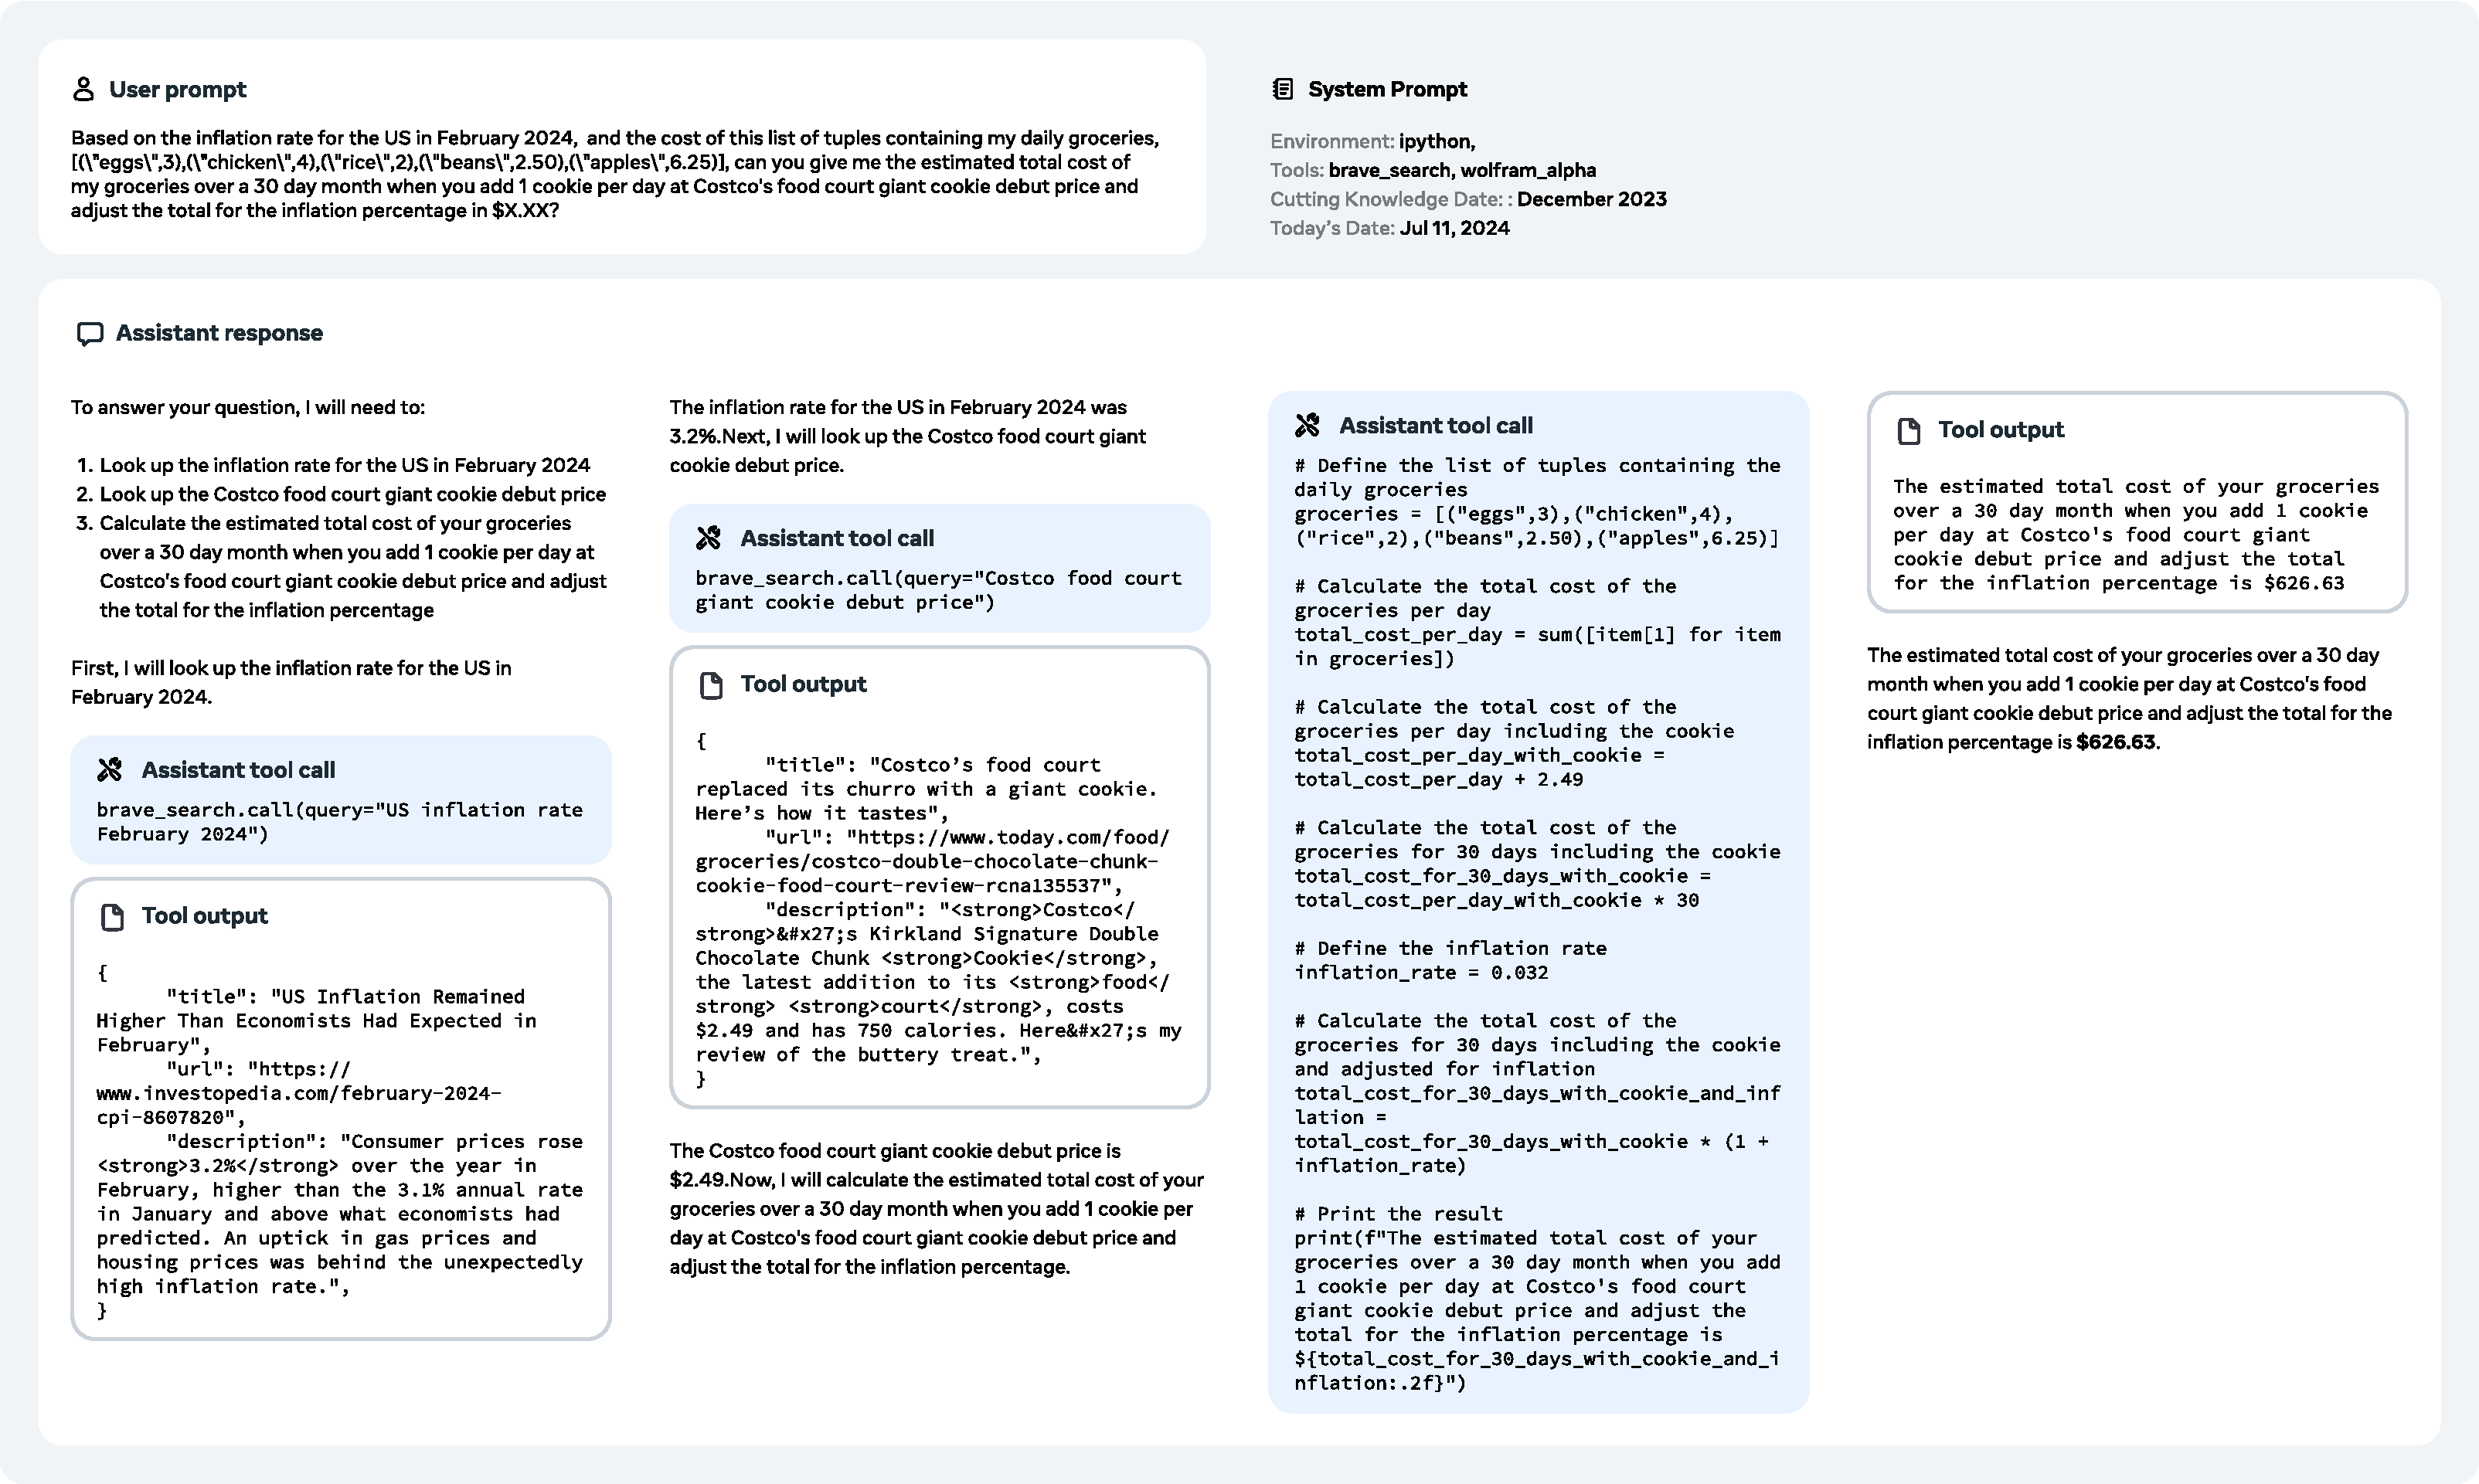
\includegraphics[width=\textwidth]{assets/llama-search-code.pdf}
    \caption{\textbf{Multi-step tool usage.} Example of \llamathree performing multi-step planning, reasoning, and tool calling to solve a task.}
    \label{fig:multi_step_tool_use}
\end{figure}

\textbf{Zero-shot tool use data.}
We improve \llamathree~zero-shot tool use abilities (also referred to as function calling) by finetuning on a large and diverse set of partly synthetic (functions definitions, user query, corresponding call) tuples. We evaluate our model on a set of unseen tools. 
\begin{itemize}
    \item \textbf{Single, nested, and parallel function calling:} %
    Calls can be simple, nested, \textit{i.e.} we pass a function call as an argument of another function, or parallel, \textit{i.e.} the model returns a list of independent function calls. Generating a diverse set of functions, queries and ground truths can be challenging~\citep{mekala2024toolverifier}, and we resort to mining the Stack~\citep{kocetkov2022stack3tbpermissively} to ground our synthetic user queries in real functions. More precisely, we extract function calls and their definitions, clean and filter them, \textit{e.g.} for missing docstrings or non-executable functions, and use \llamathree~to generate a natural language query corresponding to the function call. 

    \item \textbf{Multi-turn function calling:}  We also generate synthetic data for multi-turn dialogs with function calls, following a protocol similar to the one proposed in~\cite{li2023api}. We use multiple agents that generate domains, APIs, user queries, API calls, and responses, while also ensuring that the generated data covers a set of diverse domains and realistic APIs. All agents are variants of \llamathree~prompted in different ways depending on their roles and collaborate in a step-by-step manner. %
    

\begin{figure}[t]
    \centering
    \includegraphics[width=\textwidth]{assets/llama-file-upload-6x.png}
    \caption{\textbf{Processing file uploads.} Example of \llamathree performing analysis and visualization of an uploaded file.}
    \label{fig:file_upload}
\end{figure}

\end{itemize}

\subsubsection{Factuality}\label{subsubsec:factuality}

Hallucinations remain a major challenge for large language models. Models tend to be overconfident, even in domains where they have little knowledge. Despite these shortcomings, they are often used as knowledge bases, which can lead to risky outcomes such as the spread of misinformation. While we recognize that factuality can go beyond hallucinations, we took a hallucination-first approach here.


We follow the principle that post-training should align the model to ``know what it knows'' rather than add knowledge~\citep{gekhman2024does,mielke2020metacognition}. Our primary approach involves generating data that aligns model generations with subsets of factual data present in the pre-training data. To achieve this, we develop a knowledge probing technique that takes advantage of \llamathree's in-context abilities. This data generation process involves the following procedure:

\begin{enumerate}
    \item \textbf{Extract a data snippet} from the pre-training data. %
    \item \textbf{Generate a factual question} about these snippets (context) by prompting \llamathree.
    \item \textbf{Sample responses} from \llamathree~to the question.
    \item \textbf{Score the correctness} of the generations using the original context as a reference and \llamathree~as a judge.
    \item \textbf{Score the informativeness} of the generations using \llamathree~as a judge.
    \item \textbf{Generate a refusal} for responses which are consistently informative and incorrect across the generations, using \llamathree.
\end{enumerate}

We use data generated from the knowledge probe to encourage the model to only answer questions which it has knowledge about, and refuse answering those questions that it is unsure about. %
Further, pre-training data is not always factually consistent or correct. We therefore also collect a limited set of labeled factuality data that deals with sensitive topics where factually contradictory or incorrect statements are prevalent. %

\subsubsection{Steerability}
\label{subsubsec:steerability}

Steerability is the ability to direct the model's actions and outcomes to meet developer and user specifications. As \llamathree is a generic foundational model, it should be maximally steerable to different downstream use cases easily. For \llamathree, we focus on enhancing its steerability through system prompt with natural language instructions, especially around response length, format, tone and character/persona. 

\textbf{Data collection.}  We collect steerability preference samples within the general English category by asking annotators to design different system prompts for \llamathree. Annotators then engage in conversations with the models to evaluate their consistency in following instructions defined in system prompts over the course of the conversation. We show an example customized system prompt used for enhancing steerability below:


\begin{tcolorbox}
\texttt{You are a helpful and cheerful AI Chatbot that acts as a meal plan assistant for busy families. The family consists of 2 adults, 3 teenagers, and 2 preschoolers. Plan two or three days at a time and use leftovers or extra ingredients for the second day's plan. The user will let you know if they want two or three days. If they don't, assume three days. Each plan should include breakfast, lunch, snack, and dinner. Ask the user if they approve of the plan or need adjustments. After they approve provide a grocery list with family size in mind. Always keep family preferences in mind and if there's something that they don't like provide a substitution. If the user is not feeling inspired then ask them what's the one place they wish they could visit on vacation this week and then suggest meals based on that location's culture. Weekend meals can be more complex. Weekday meals should be quick and easy. For breakfast and lunch, easy food like cereal, English muffins with pre-cooked bacon, and other quick easy foods are preferred. The family is busy. Be sure to ask if they have essentials and favorites on hand like coffee or energy drinks so they don't forget to buy it. Remember to be budget-conscious unless it's a special occasion.}
\end{tcolorbox}

\textbf{Modeling.} After we collect the preference data, we leverage this data in reward modeling, rejection sampling, SFT, and DPO to enhance \llamathree's steerability. 

\section{Empirical Evaluation}
We trained a series of models of various sizes. For all subsequent evaluations, we will use the largest model (referred to as CogVideoX).
In this section, we present the experimental validation of CogVideoX through two primary methods: automated metric evaluation and human assessment, providing a thorough analysis of the performance and quality of the generated videos. 
We trained a series of models with different parameter sizes. The following evaluation defaults to using our largest model.

\subsection{Results of Automated Metric Evaluation} 

\paragraph{Baselines.} We chose several top-performing text-to-video models as our baselines for comparison, including T2V-Turbo~\citep{li2024t2v}, AnimateDiff~\citep{guo2023animatediff}, VideoCrafter2~\citep{chen2024videocrafter2}, OpenSora~\citep{opensora}, Show-1~\citep{zhang2023show}, Gen-2~\citep{gen2}, Pika~\citep{pika} and LaVie-2~\citep{wang2023lavie}.


% \begin{figure}[h]
% \begin{center}
% \includegraphics[width=0.9\linewidth]{images/bench_eval.png}
% \end{center}
% \caption{The radar chart comparing the performance of different models.}
% \label{fig:radar}
% \end{figure}

\hide{
%\begin{wrapfigure}{r}{0.5\textwidth}
\begin{figure}
\centering
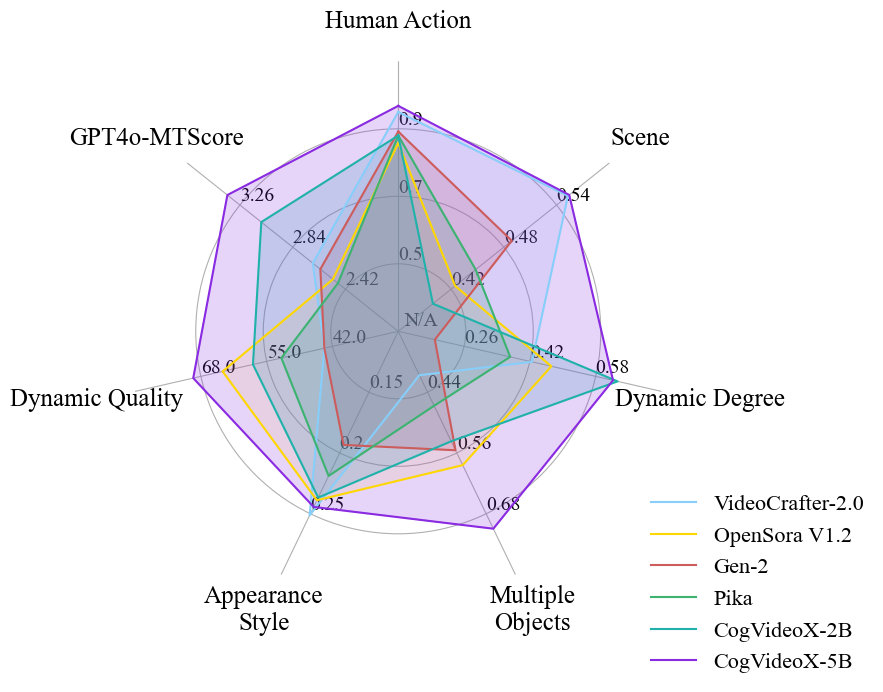
\includegraphics[width=0.7\linewidth]{images/bench_eval9.png}
\caption{The radar chart comparing the performance of different models. CogVideoX represents the largest one. It is clear that CogVideoX outperforms its competitors in the vast majority of metrics, and it is very close to the leading models in the remaining indicator.
}
\label{fig:radar}
% \vspace{-10mm}
%\end{wrapfigure}

\end{figure}

}%end ofhide
\paragraph{Evaluation Metrics.} To evaluate the text-to-video generation, we employed several metrics from VBench~\citep{huang2023vbench}: \emph{Human Action}, \emph{Scene}, \emph{Dynamic Degree}, \emph{Multiple Objects}, and \emph{Appearance Style}. VBench is a suite of tools designed to automatically assess the quality of generated videos. We have selected certain metrics from VBench, excluding others that do not align with our evaluation needs. For example, the color metric, intended to measure the presence of objects corresponding to specific colors across frames in the generated video, assesses the model's quality by calculating the probability. However, this metric may mislead video generation models that exhibit greater variation, thus we chose not to include it in our evaluation. For longer-generated videos, some models might produce videos with minimal changes between frames to obtain higher scores, but these videos lack rich content. Therefore, a metric for evaluating the dynamism of the video becomes more important. To address this, we employed two video evaluation tools, We also employed the \emph{Dynamic Quality} from Devil~\citep{liao2024evaluationtexttovideogenerationmodels} and \emph{GPT4o-MTScore} from ChronoMagic~\citep{yuan2024chronomagic}, which focus more on the dynamic characteristics of videos. \emph{Dynamic Quality} is defined by the integration of various quality metrics with dynamic scores. This approach mitigates biases arising from negative correlations between video dynamics and video quality, leading to a more thorough assessment of video quality. ChronoMagic, for instance, introduces the \emph{GPT4o-MTScore}, a metric designed to measure the metamorphic amplitude of time-lapse videos, such as those depicting physical, biological, and meteorological changes. This metric is obtained by extracting frames from the generated videos at regular intervals and using GPT-4o~\citep{gpt4o} to score the degree of change, providing a fine-grained assessment of video dynamism. This method ensures a more accurate evaluation of the content's variability over time, countering the potential bias of static frame sequences in scoring.



\paragraph{Results.} Table~\ref{table:results} provides a detailed comparison of the performance of our CogVideoX model with other models. Our model achieved the best performance in 5 out of the 7 metrics and showed competitive results in the remaining 2 metrics. These results demonstrate that our model not only excels in video generation quality but also outperforms previous models in handling various complex dynamic scenes. Additionally, Figure~\ref{fig:radar} presents a radar chart comparing the performance of different models.


\begin{figure}[ht]
\begin{center}
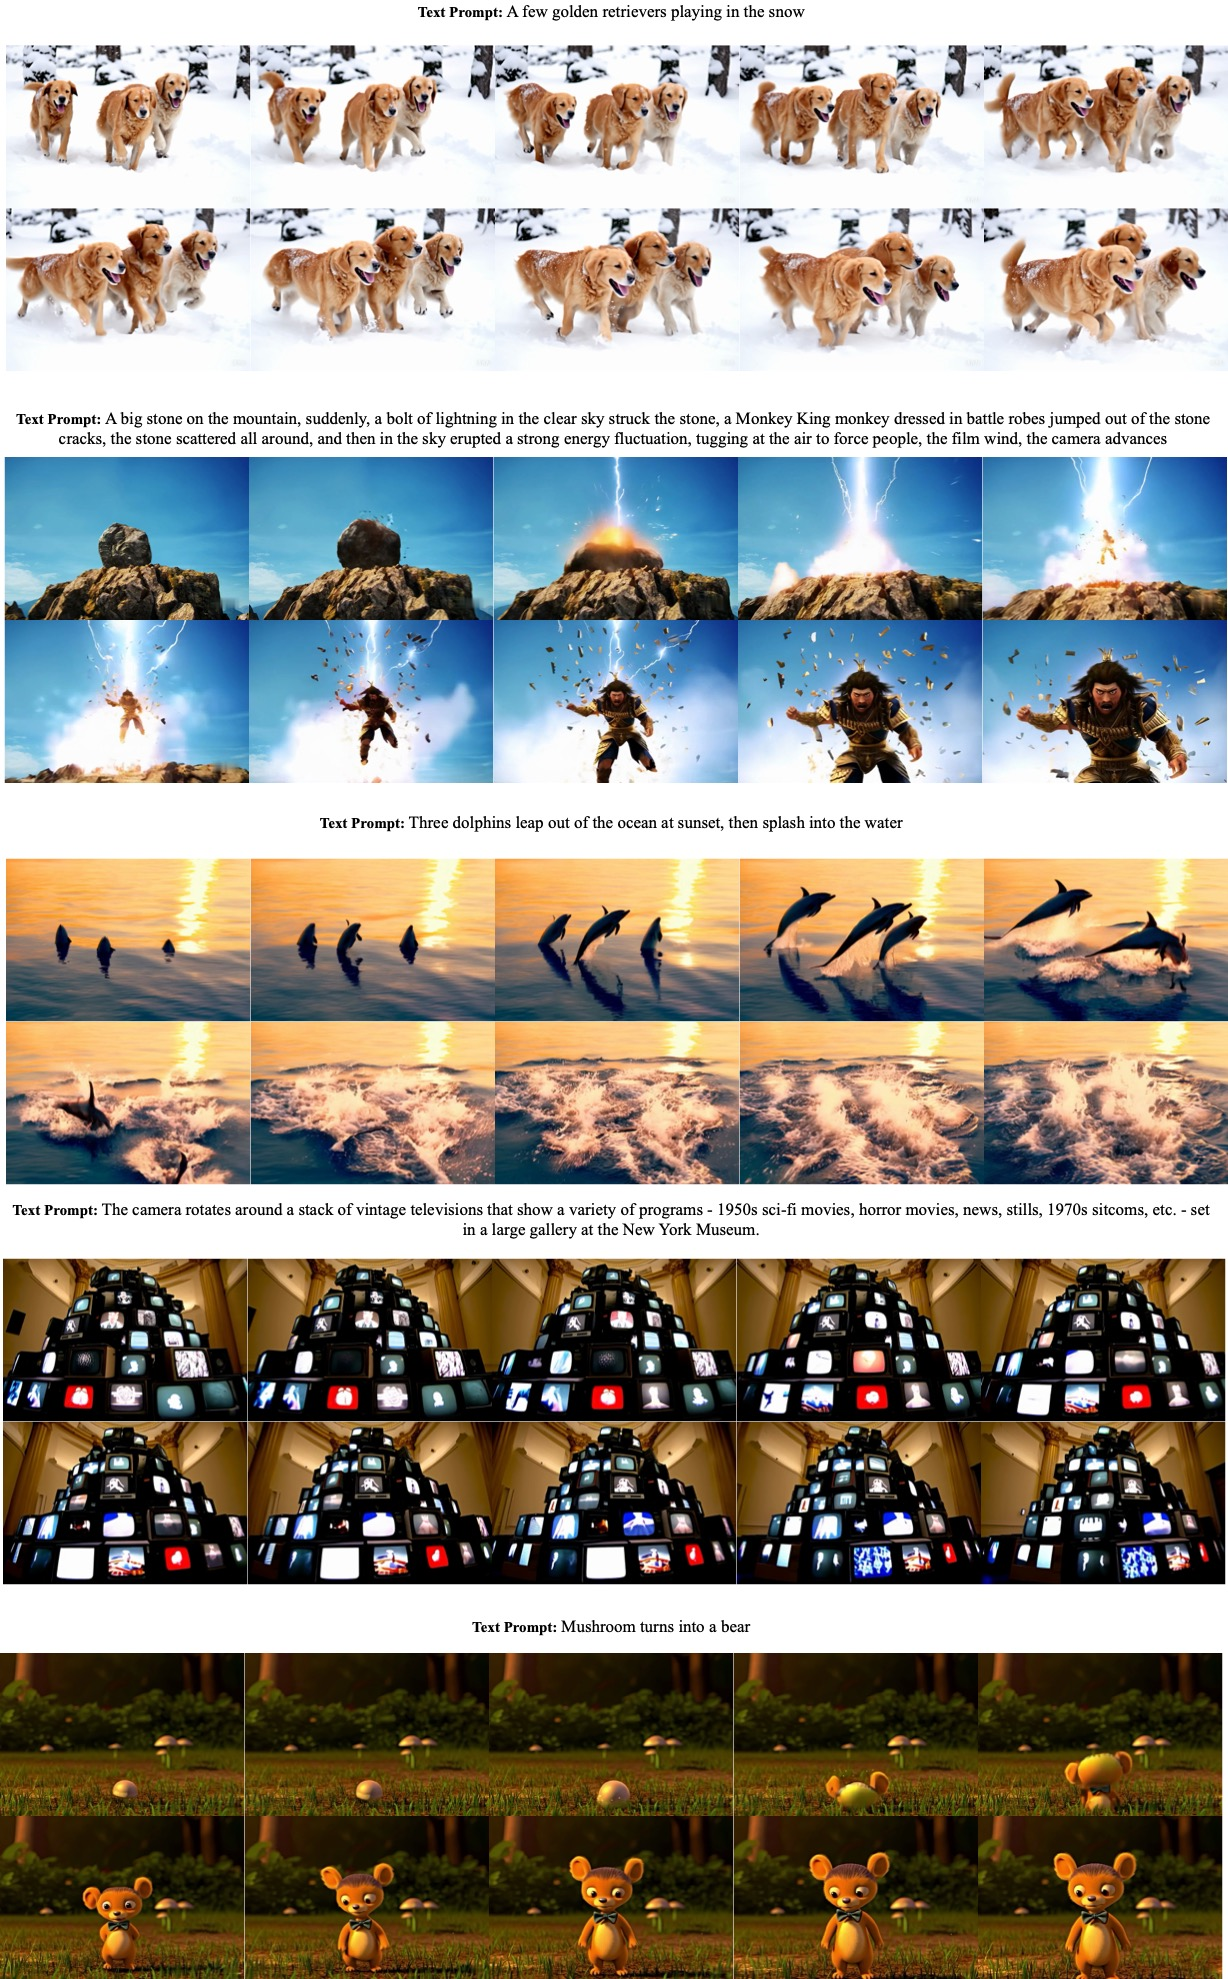
\includegraphics[width=\linewidth]{images/t2v/goodcase1.jpg}
\end{center}
\caption{Text to video showcases. The displayed prompt will be upsampled before being fed into the model. The generated videos contain large motion and can produce various video styles.}
\label{fig:t2vgood1}
\end{figure}

\begin{figure}[ht]
\begin{center}
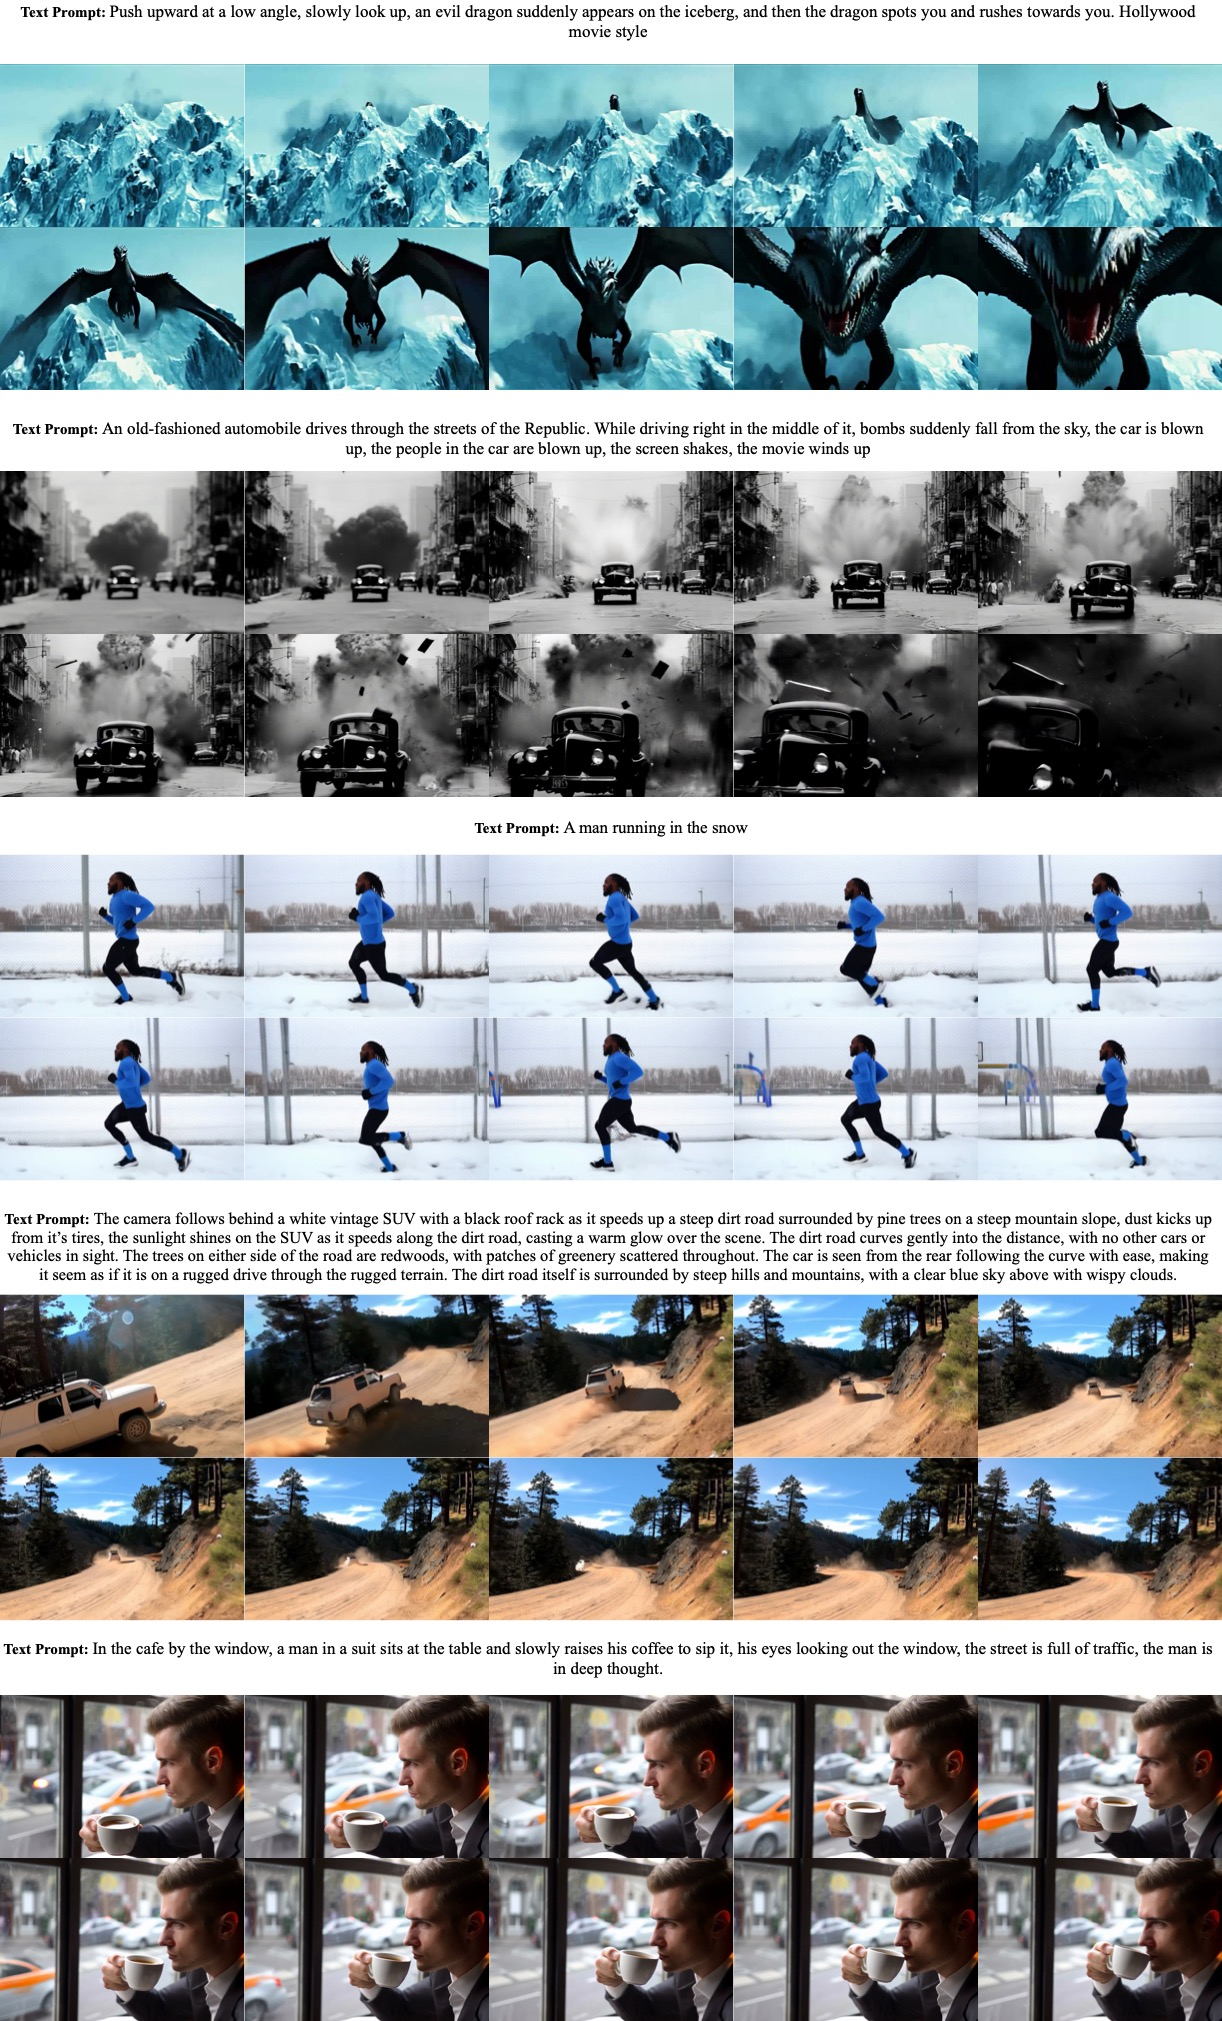
\includegraphics[width=0.98\linewidth]{images/t2v/goodcase2.jpg}
\end{center}
\caption{Text to video showcases.}
\label{fig:t2vgood2}
\end{figure}


% Please add the following required packages to your document preamble:
% \usepackage[table,xcdraw]{xcolor}
% Beamer presentation requires \usepackage{colortbl} instead of \usepackage[table,xcdraw]{xcolor}
% \usepackage[normalem]{ulem}
% \useunder{\uline}{\ul}{}




% \begin{table}[]

% \centering
% \setlength\tabcolsep{3pt}

% \label{sample-table}
% \small
% \vspace{-10pt}
% \caption{\textbf{Automatic Evaluation Results per Dimension.}The table presents a comparative analysis of various video models across different dimensions. It is evident from the table that, in terms of both human motion and background effects as well as the accuracy and distinctiveness of objects, CogVideoX has achieved the current SOTA level. Furthermore, CogVideoX has garnered a commendable score in the expression of dynamic qualities, a capability that serves as a more precise indicator of the intrinsic properties of video media, distinct from the static nature of photographic images.}

% \vspace{6pt}

% \begin{tabular}{cccccccc}
% \toprule
% \multirow{2}{*}{\textbf{Models} }  & \textbf{human}  & \textbf{object} &\multirow{2}{*}{\textbf{scene}}&\textbf{dynamic} &\textbf{multiple} &\textbf{spatial} &\textbf{appearance} \\
%     & \textbf{action}& \textbf{class}& & \textbf{degree} &\textbf{objects}& \textbf{relationship}&\textbf{style}  
% \\
% \midrule
% CogVideoX & 96.80\% &93.70\% & 55.44\% & 62.22\% & 70.95\% & 61.29\% & 24.44\% \\
% {LaVie-2} & 96.40\% & 97.52\%  & 49.59\% & 31.11\% & 64.88\%  & 38.68\% & 25.09\%  \\
% {T2V-Turbo}  & 95.20\%  & 93.96\%& 55.58\% & 49.17\% & 54.65\%    & 38.67\%  & 24.42\%   \\
% {Gen-2}  & 89.20\%& 90.92\%  & 48.91\%  & 18.89\% & 55.47\%    & 66.91\%   & 19.34\%  \\
% {VideoCrafter-2.0\citep{chen2024videocrafter2}} & 95.00\% & 92.55\% & 55.29\%               & 42.50\% & 40.66\% & 35.86\% & 25.13\%  \\
% {Pika Beta} & 88.00\% & 87.45\%  & 44.80\% & 37.22\% & 46.69\% & 65.65\% & 21.89\%   \\
% AnimateDiff-V2 & 92.60\% & 90.90\%  & 50.19\% & 40.83\%        & 36.88\% & 34.60\%  & 22.42\%\\
% {OpenSora V1.2}   & 85.80\% & 83.37\%& 42.47\%   & 47.22\%    & 58.41\% & 67.51\%  & 23.89\%  \\
% {Show-1} & 95.60\%  & 93.07\%  & 47.03\% & 44.44\% & 45.47\% & 53.50\%  & 23.06\%  \\
% {HiGen}  & 86.20\%  & 86.06\%  & 44.88\% & 99.17\% & 22.39\%  & 22.43\% & 24.54\% \\  
% \bottomrule
% \end{tabular}
% \end{table}



% \iffalse



% \begin{table}[ht!]
% \centering
% \caption{Evaluation results.}
% \setlength\tabcolsep{3pt}
% \label{sample-table}
% \begin{center}
% \small
% \resizebox{0.9\linewidth}{!}{
% \begin{tabular}{ccccccccc}

% \multirow{2}{*}{\textbf{Models} }  & \textbf{subject}  & \textbf{background} &\textbf{temporal} &\textbf{motion} &\textbf{dynamic} &\textbf{aesthetic} &\textbf{imaging} &\textbf{object} \\
%     & \textbf{consistency}& \textbf{consistency}& \textbf{flickering}& \textbf{smoothness} &\textbf{degree}& \textbf{quality}&\textbf{quality} & \textbf{class}
% \\ \hline 
%         CogVideoX & 94.66\% & 95.92\% & 97.47\% & 98.10\% & 62.22\% & 55.14\% & 63.62\% & 93.70\%  \\
%         LaVie-2 & 97.90\% & 98.45\% & 98.76\% & 98.42\% & 31.11\% & 67.62\% & 70.39\% & 97.52\%  \\ 
%         T2V-Turbo (VC2) & 96.28\% & 97.02\% & 97.48\% & 97.34\% & 49.17\% & 63.04\% & 72.49\% & 93.96\%  \\ 
%         Gen-2 (2023-06) & 97.61\% & 97.61\% & 99.56\% & 99.58\% & 18.89\% & 66.96\% & 67.42\% & 90.92\%  \\ 
%         VideoCrafter-2.0\citep{chen2024videocrafter2} & 96.85\% & 98.22\% & 98.41\% & 97.73\% & 42.50\% & 63.13\% & 67.22\% & 92.55\%  \\ 
%         Pika Beta (2023-06) & 96.76\% & 98.95\% & 99.77\% & 99.51\% & 37.22\% & 63.15\% & 62.33\% & 87.45\%  \\ 
%         AnimateDiff-V2 & 95.30\% & 97.68\% & 98.75\% & 97.76\% & 40.83\% & 67.16\% & 70.10\% & 90.90\%  \\ 
%         OpenSora V1.2 & 94.45\% & 97.90\% & 99.47\% & 98.20\% & 47.22\% & 56.18\% & 60.94\% & 83.37\%  \\ 
%         Show-1 & 95.53\% & 98.02\% & 99.12\% & 98.24\% & 44.44\% & 57.35\% & 58.66\% & 93.07\%  \\ 
%         HiGen & 90.07\% & 93.99\% & 93.24\% & 96.69\% & 99.17\% & 57.30\% & 63.92\% & 86.06\% \\ 
% \hline \\

% \multirow{2}{*}{\textbf{Models} }  & \textbf{multiple}  & \textbf{human} &\multirow{2}{*}{\textbf{color}} &\textbf{spatial} &\multirow{2}{*}{\textbf{scene}} &\textbf{appearance} &\textbf{temporal} &\textbf{overall} \\
%     & \textbf{objects}& \textbf{action}& & \textbf{relation} & & \textbf{style}&\textbf{style} & \textbf{consistency}
% \\ \hline 
%         CogVideoX & 70.95\% & 96.80\% & 79.75\% & 61.29\% & 55.44\% & 24.44\% & 23.69\% & 26.73\%  \\ 
%         LaVie-2 & 64.88\% & 96.40\% & 91.65\% & 38.68\% & 49.59\% & 25.09\% & 25.24\% & 27.39\%  \\ 
%         T2V-Turbo (VC2) & 54.65\% & 95.20\% & 89.90\% & 38.67\% & 55.58\% & 24.42\% & 25.51\% & 28.16\%  \\
%         Gen-2 (2023-06) & 55.47\% & 89.20\% & 89.49\% & 66.91\% & 48.91\% & 19.34\% & 24.12\% & 26.17\%  \\ 
%         VideoCrafter-2.0 & 40.66\% & 95.00\% & 92.92\% & 35.86\% & 55.29\% & 25.13\% & 25.84\% & 28.23\%  \\
%         Pika Beta (2023-06) & 46.69\% & 88.00\% & 85.31\% & 65.65\% & 44.80\% & 21.89\% & 24.44\% & 25.47\%  \\ 
%         AnimateDiff-V2 & 36.88\% & 92.60\% & 87.47\% & 34.60\% & 50.19\% & 22.42\% & 26.03\% & 27.04\%  \\ 
%         OpenSora V1.2 & 58.41\% & 85.80\% & 87.49\% & 67.51\% & 42.47\% & 23.89\% & 24.55\% & 27.07\%  \\ 
%         Show-1 & 45.47\% & 95.60\% & 86.35\% & 53.50\% & 47.03\% & 23.06\% & 25.28\% & 27.46\%  \\ 
%         HiGen & 22.39\% & 86.20\% & 86.22\% & 22.43\% & 44.88\% & 24.54\% & 25.14\% & 27.14\% \\ \hline

% \hline \\
% \end{tabular}

% }
% \end{center}
% \end{table}

% \fi






% \begin{table}[!ht]
% \centering

% \label{sample-table}
% \small
% \vspace{-10pt}
% \caption{\textbf{Automatic Evaluation Results per Dimension.}}

% \vspace{6pt}

% \resizebox{0.8\linewidth}{!}{
%     \begin{tabular}{cccc}
%         \textbf{Models} & \textbf{\Centerstack{Dynamics Range}} & \textbf{\Centerstack{Dynamics Controllability}} & \textbf{\Centerstack{Dynamics-based Quality}} \\ \hline
%         CogVideoX       & 55.7 & 71.8 & \textbf{69.5} \\ 
%         Gen-2           & 30.8 & \textbf{82.5} & 43.6 \\ 
%         Pika            & 43.2 & 72.0 & 52.1 \\ 
%         VideoCrafter2   & 34.1 & 57.0 & 43.6 \\ 
%         OpenSora        & \textbf{61.2} & 62.4 & 63.7 \\ 
%         Show-1          & 45.1 & 73.9 & 57.7 \\ 
%     \end{tabular}
% }
% \end{table}


% \begin{figure}[h]
% \begin{center}
% \includegraphics[width=0.9\linewidth]{images/bench_eval.png}
% \end{center}
% \caption{The radar chart comparing the performance of different models.}
% \label{fig:radar}
% \end{figure}

\hide{
%\begin{wrapfigure}{r}{0.5\textwidth}
\begin{figure}
\centering
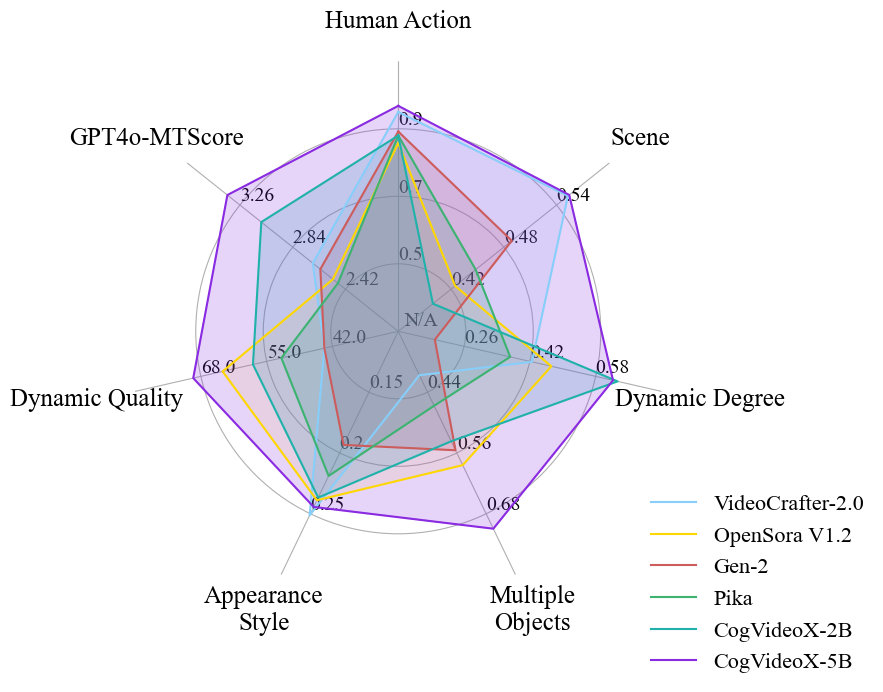
\includegraphics[width=0.7\linewidth]{images/bench_eval9.png}
\caption{The radar chart comparing the performance of different models. CogVideoX represents the largest one. It is clear that CogVideoX outperforms its competitors in the vast majority of metrics, and it is very close to the leading models in the remaining indicator.
}
\label{fig:radar}
% \vspace{-10mm}
%\end{wrapfigure}

\end{figure}

}%end ofhide


\subsection{Human Evaluation}
In addition to automated scoring mechanisms, a comparative analysis between the Kling~\citep{kling} and CogVideoX was conducted using a manual scoring system. One hundred meticulously crafted prompts were used, characterized by their broad distribution, clear articulation, and well-defined conceptual scope. We randomize videos for blind evalution. A panel of evaluators assigned scores for each detail on a scale from zero to one, with the overall total score rated on a scale from zero to five, where higher scores reflect better video quality. Reasons for any score deductions were also carefully documented. The results shown in Table~\ref{table:human_eva} indicate that our model outperforms Kling in all aspects. More details are shown in \ref{sec:human_evalution}.

\begin{table}[!ht]
\centering
\label{sample-table}
\small
\vspace{-5pt}
\caption{Human evaluation between CogVideoX and Kling.}
\label{table:human_eva}
\resizebox{0.75\linewidth}{!}{
    \begin{tabular}{cccccc}
    \toprule
        Model & \Centerstack{Sensory\\Quality} & \Centerstack{Instruction\\Following}&\Centerstack{Physics\\Simulation} & \Centerstack{Cover\\Quality} & 
        \Centerstack{Total\\Score} \\ 
        \midrule
        Kling & 0.638 & 0.367 & 0.561 & 0.668 & 2.17 \\
        \midrule
         {\bf CogVideoX-5B} & {\bf 0.722} & {\bf 0.495} & {\bf 0.667} & {\bf 0.712} & {\bf 2.74}  \\
        \bottomrule
    \end{tabular}
}
\vspace{-3mm}
\end{table}



% \begin{table}[!ht]
% \centering

% \label{sample-table}
% \small
% \vspace{-10pt}
% \caption{\textbf{Automatic Evaluation Results per Dimension.}}

% \vspace{6pt}

% \resizebox{0.8\linewidth}{!}{
%     \begin{tabular}{cccc}
%         \textbf{Models} & \textbf{\Centerstack{Dynamics Range}} & \textbf{\Centerstack{Dynamics Controllability}} & \textbf{\Centerstack{Dynamics-based Quality}} \\ \hline
%         CogVideoX       & 55.7 & 71.8 & \textbf{69.5} \\ 
%         Gen-2           & 30.8 & \textbf{82.5} & 43.6 \\ 
%         Pika            & 43.2 & 72.0 & 52.1 \\ 
%         VideoCrafter2   & 34.1 & 57.0 & 43.6 \\ 
%         OpenSora        & \textbf{61.2} & 62.4 & 63.7 \\ 
%         Show-1          & 45.1 & 73.9 & 57.7 \\ 
%     \end{tabular}
% }
% \end{table}

\section{Inference}
\label{section:inference}
We investigate two main techniques to make inference with the Llama 3 405B model efficient: \textbf{(1)} pipeline parallelism and \textbf{(2)} FP8 quantization.
We have publicly released our implementation of FP8 quantization.

\subsection{Pipeline Parallelism}
\label{section:pp}

When using a BF16 number representation for the model parameters, \llamathree 405B does not fit in the GPU memory of a single machine with 8 Nvidia H100 GPUs. 
To address this issue, we parallelize model inference using BF16 precision across 16 GPUs on two machines.
Within each machine, the high NVLink bandwidth enables the use of tensor parallelism \citep{shoeybi2019megatron}. 
Across nodes, however, connectivity has lower bandwidth and higher latency, so we use pipeline parallelism \citep{huang2019gpipe} instead.

During training with pipeline parallelism, bubbles are a major efficiency concern (see Section~\ref{section:pretraining_model_scaling}).
However, they are not an issue during inference, since inference does not involve a backward pass that requires a pipeline flush. 
Therefore, we use micro-batching to improve inference throughput with pipeline parallelism. 

We evaluate the effect of using two micro-batches in inference workloads of 4,096 input tokens and 256 output tokens both during the key-value cache \emph{pre-fill} stage of inference and during the \emph{decoding} stage.
We find that micro-batching improves throughput of inference with the same local batch size; see Figure~\ref{figure:micro-batching}.
These improvements result from micro-batching enabling concurrent execution of micro batches in both these stages.
The additional synchronization points due to micro-batching also increase latency but, overall, micro-batching still leads to a better throughput-latency trade-off.

\begin{figure}
\centering
\begin{subfigure}{.5\textwidth}
  \centering
  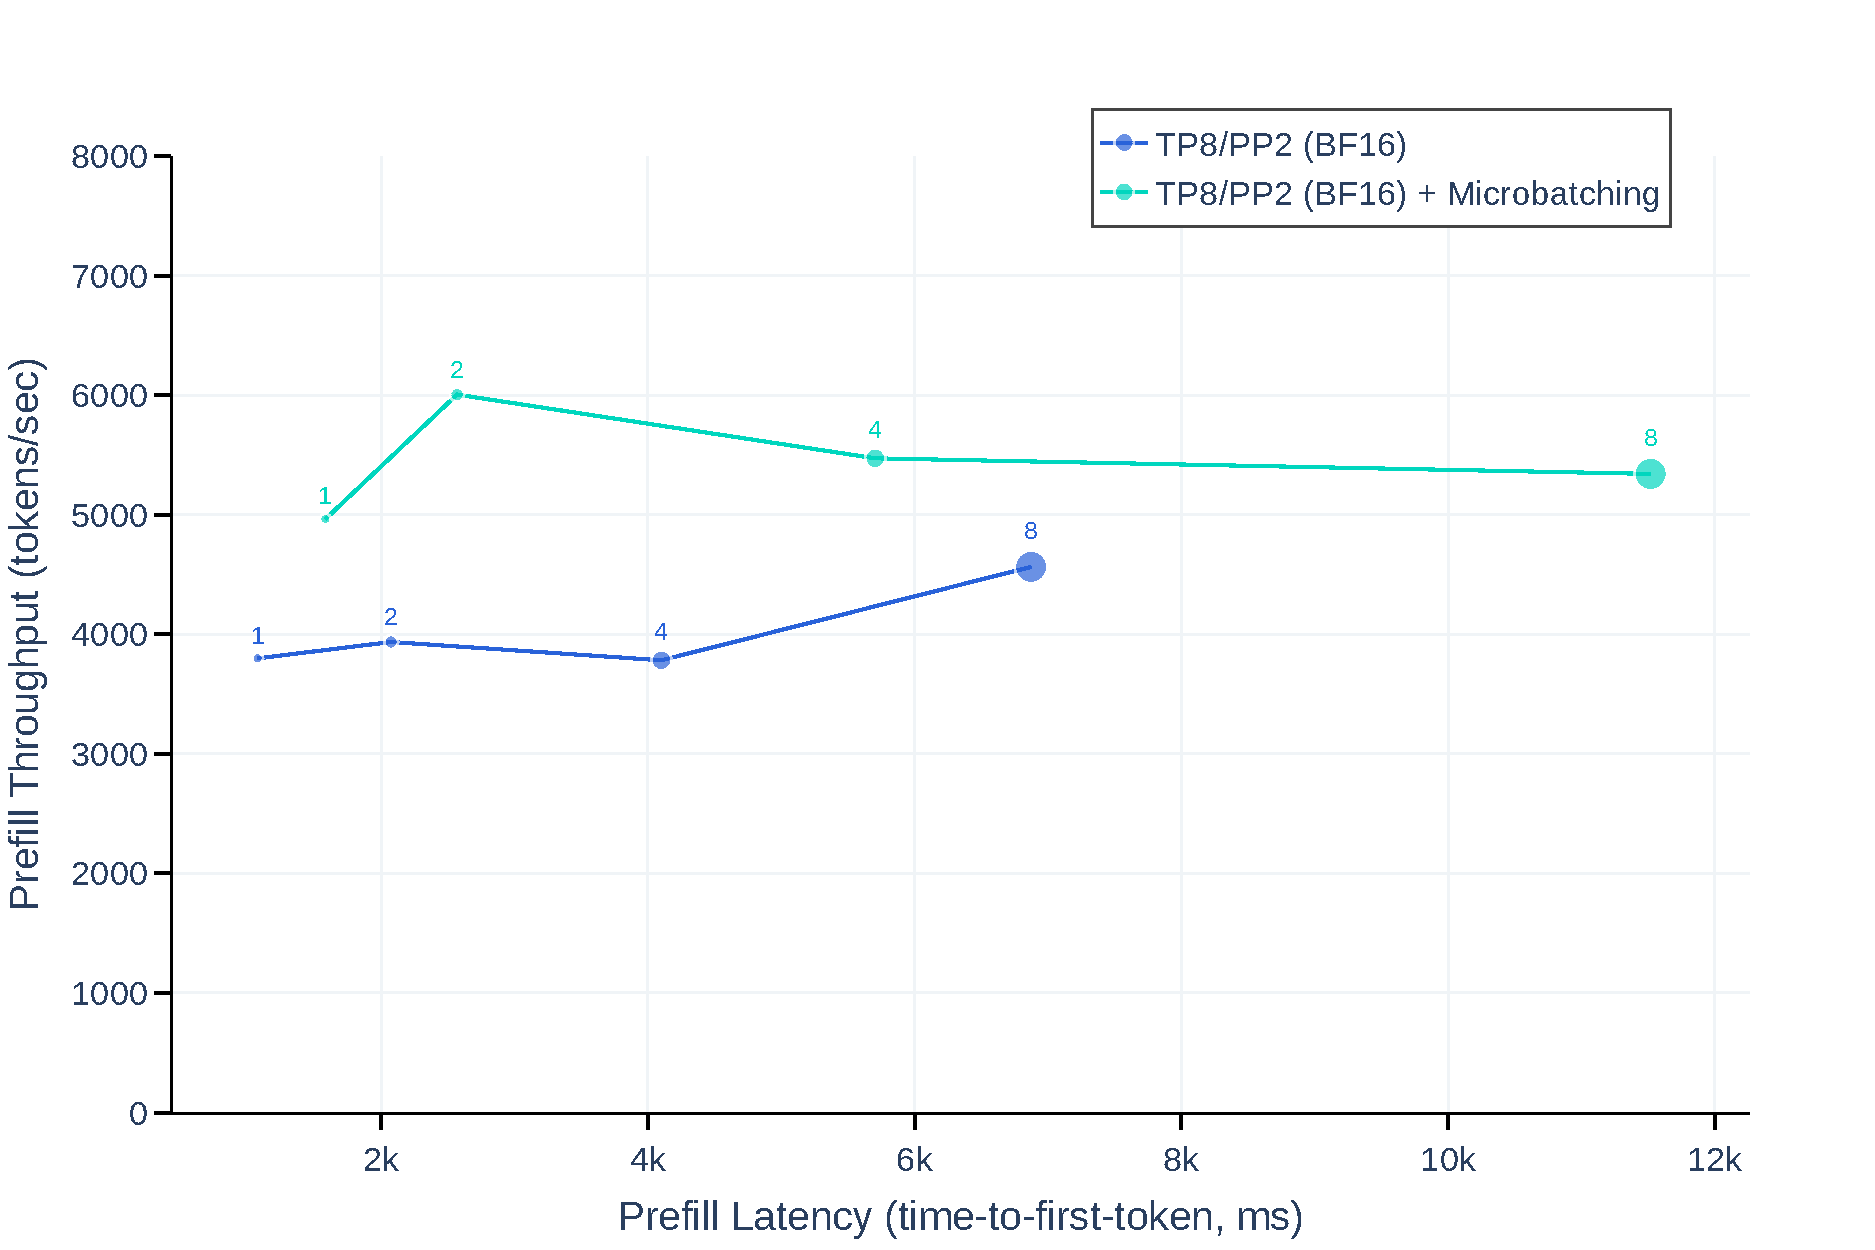
\includegraphics[width=\linewidth]{assets/prefill_micro.pdf}
\end{subfigure}%
\begin{subfigure}{.5\textwidth}
  \centering
  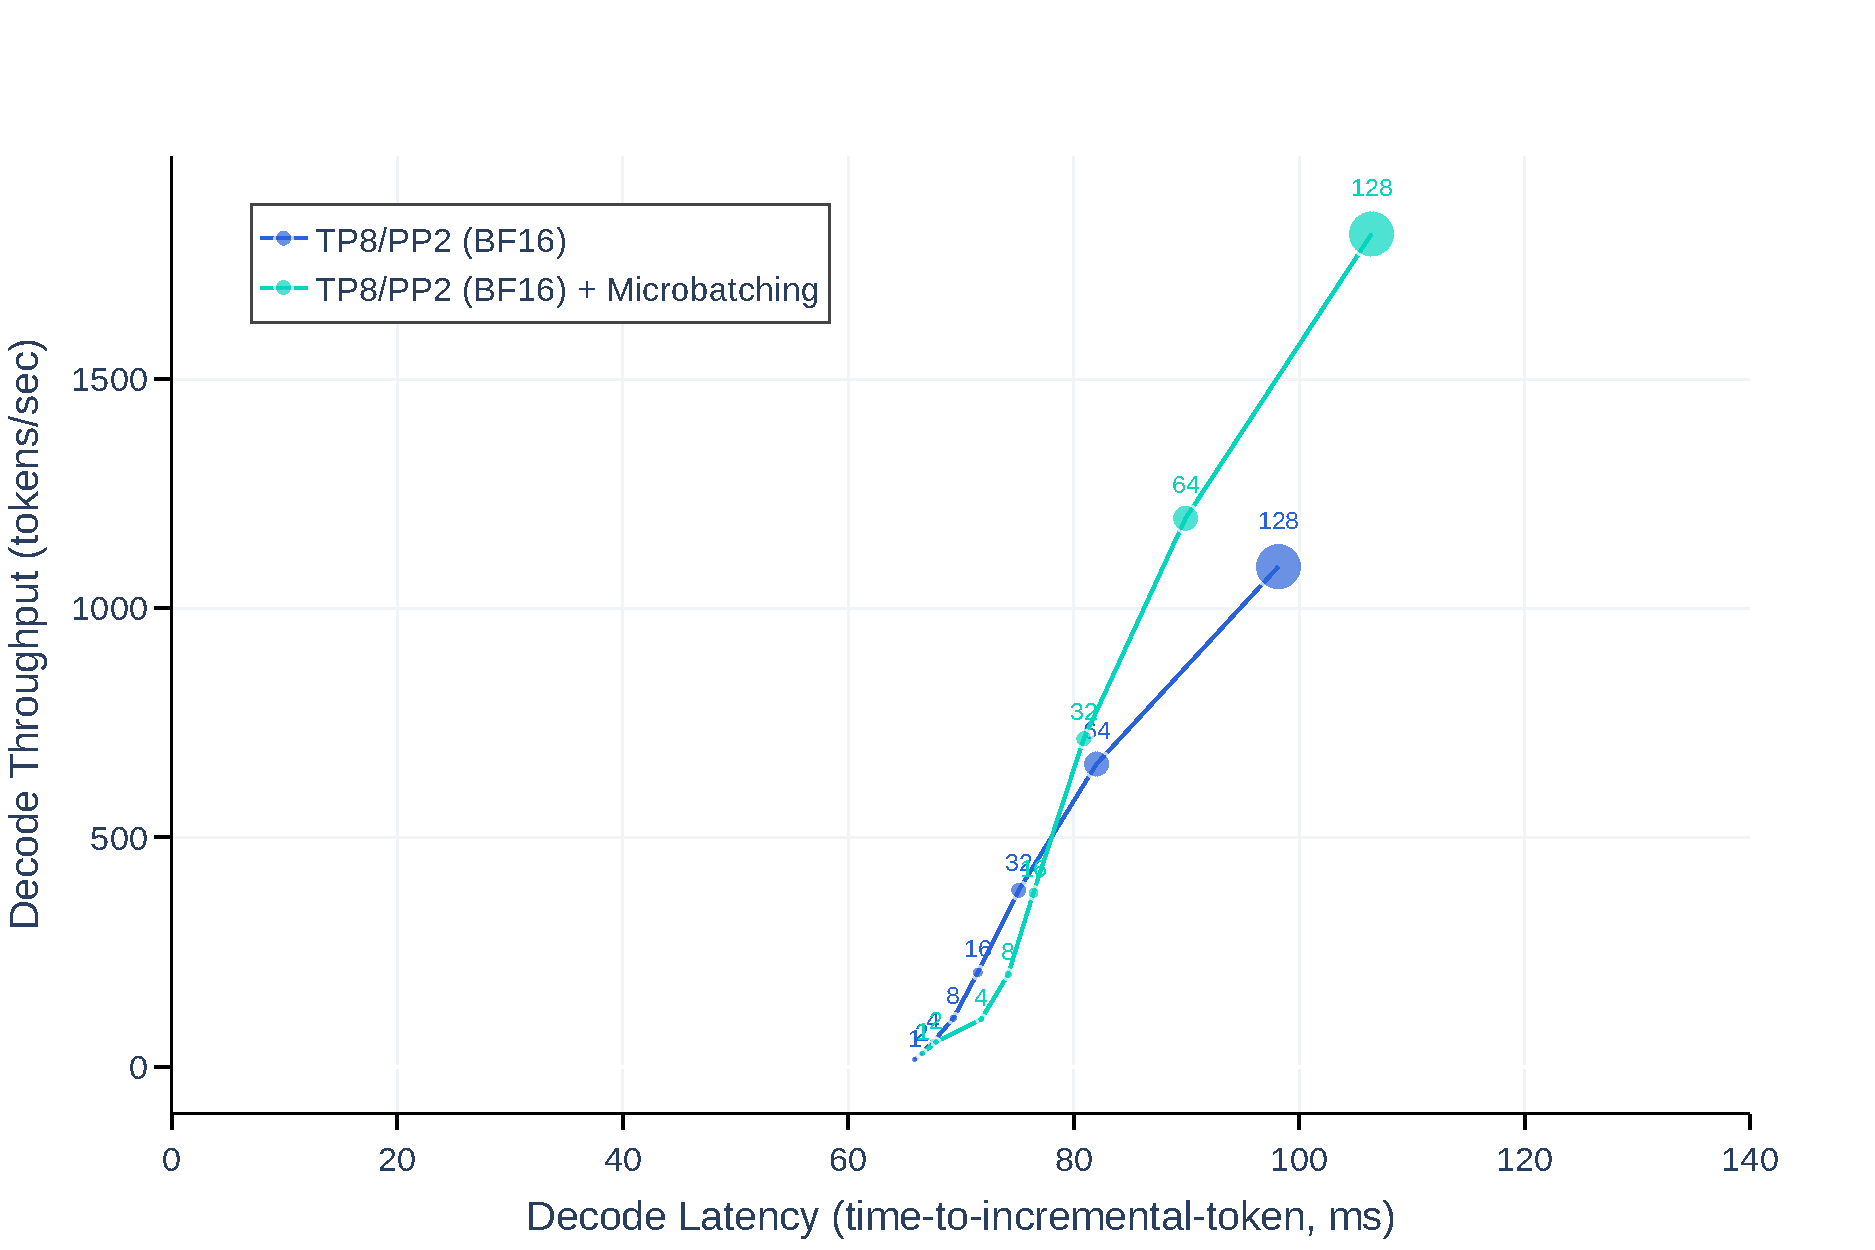
\includegraphics[width=\linewidth]{assets/decode_micro.pdf}
\end{subfigure}
\caption{\textbf{Effect of micro-batching on inference throughput and latency} during the \emph{Left:} pre-filling and \emph{Right:} decoding stage. The numbers in the plot correspond to the (micro-)batch size.}

\label{figure:micro-batching}
\end{figure}



\subsection{FP8 Quantization}
\label{section:fp8}
We perform experiments leveraging the native FP8 support of H100 GPUs to perform low-precision inference.
To enable low-precision inference, we apply FP8 quantization to most matrix multiplications inside the model.
In particular, we quantize most parameters and activations in the feedforward network layers in the model, which account for roughly 50\% of the inference compute time.
We do not quantize parameters in the self-attention layers of the model.
We leverage dynamic scaling factors for better accuracy~\citep{xiao2024smoothquant}, optimizing our CUDA kernels\footnote{Our FP8 kernels are available at \url{https://github.com/pytorch/FBGEMM/tree/main/fbgemm_gpu/experimental/gen_ai}. We provide usage examples at \url{https://github.com/meta-llama/llama-agentic-system}.} to reduce the overhead of calculating the scales.
We find that the quality of \llamathree 405B is sensitive to certain types of quantization, and make a few additional changes to increase the model output quality:

\begin{enumerate}
    \item Akin to \cite{zhang2021training}, we do not perform quantization in the first and last Transformer layers.
    \item High-perplexity tokens such as dates can lead to large activation values. In turn, these can lead to high dynamic scaling factors in FP8 and a non-negligible number of underflows, leading to errors in decoding. To address this issue, we upper bound the dynamic scaling factors to $1200$.
    \item We use row-wise quantization, computing scaling factors across rows for  parameter and activation matrices (see Figure~\ref{figure:fp8-schematic}). We find this works better than a tensor-wise quantization approach. 
\end{enumerate}

\begin{figure}[t]
\hspace*{-1.2cm}   
\centering
\includegraphics[scale=0.3]{assets/llama3-figure-25.eps}
\caption{\textbf{Illustration of tensor-wise and row-wise FP8 quantization.} \emph{Right:} Row-wise quantization enables the use of more granular activation factors than \emph{Left:} tensor-wise quantization.}
\label{figure:fp8-schematic}
\end{figure}

\textbf{Effect of quantization errors.} Evaluations on standard benchmarks often suggest that FP8 inference performs on par with BF16 inference even without these mitigations.
However, we find that such benchmarks do not adequately reflect the effects of FP8 quantization.
When scaling factors are not upper bounded, the model occasionally produces corrupted responses even though the benchmark performance is strong.
Instead of relying on benchmarks to measure distribution changes due to quantization, we find it is better to analyze the distribution of reward-model scores for $100,000$ responses produced using both FP8 and BF16.
Figure \ref{figure:reward-scores} shows the resulting reward distribution for our quantization approach.
The results in the figure show that our approach to FP8 quantization has very limited impact on the model's response. 

\begin{figure}[t]
\centering
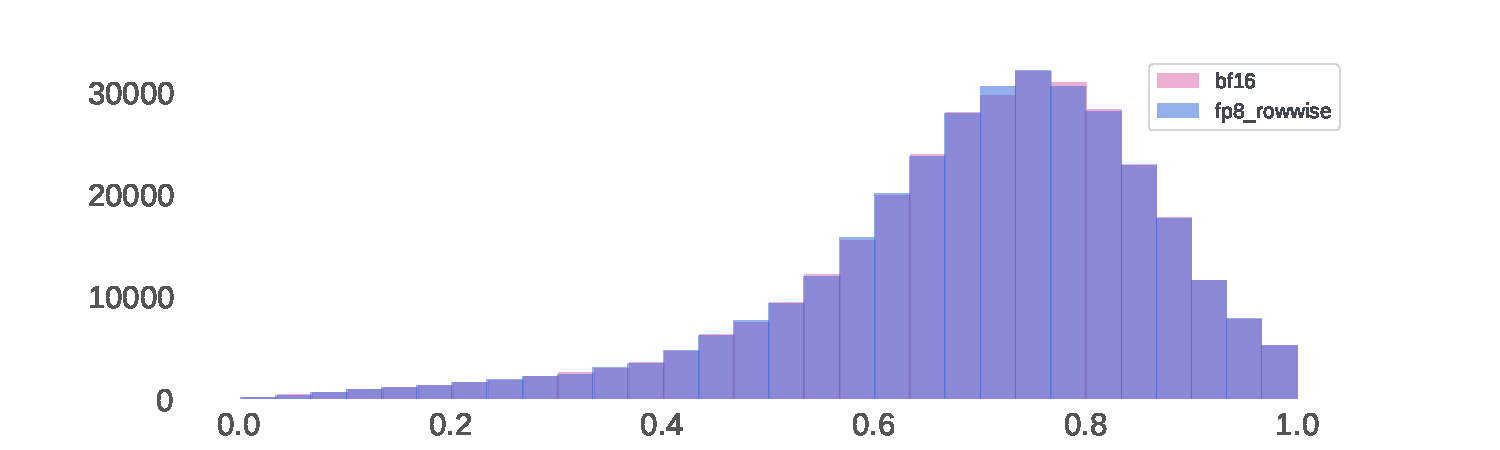
\includegraphics[scale=0.5]{assets/bf16_vs_fp8_new.pdf}
\caption{\textbf{Reward score distribution for Llama 3 405B using BF16 and FP8 inference.} Our FP8 quantization approach has negligible impact on the model's responses.}
\label{figure:reward-scores}
\end{figure}

\textbf{Experimental evaluation of efficiency.}
Figure~\ref{figure:fp8_speed} depicts the throughput-latency trade-off of performing FP8 inference with \llamathree 405B in the pre-fill and decoding stages, using 4,096 input tokens and 256 output tokens.
The figure compares the efficiency of FP8 inference with that of the two-machine BF16 inference approach described in Section~\ref{section:pp}.
The results show that use of FP8 inference leads to throughput improvements of up to 50$\%$ during the pre-fill stage, and a substantially better throughput-latency trade-off during decoding.

\begin{figure}
\centering
  \begin{subfigure}{.5\textwidth}
    \centering
    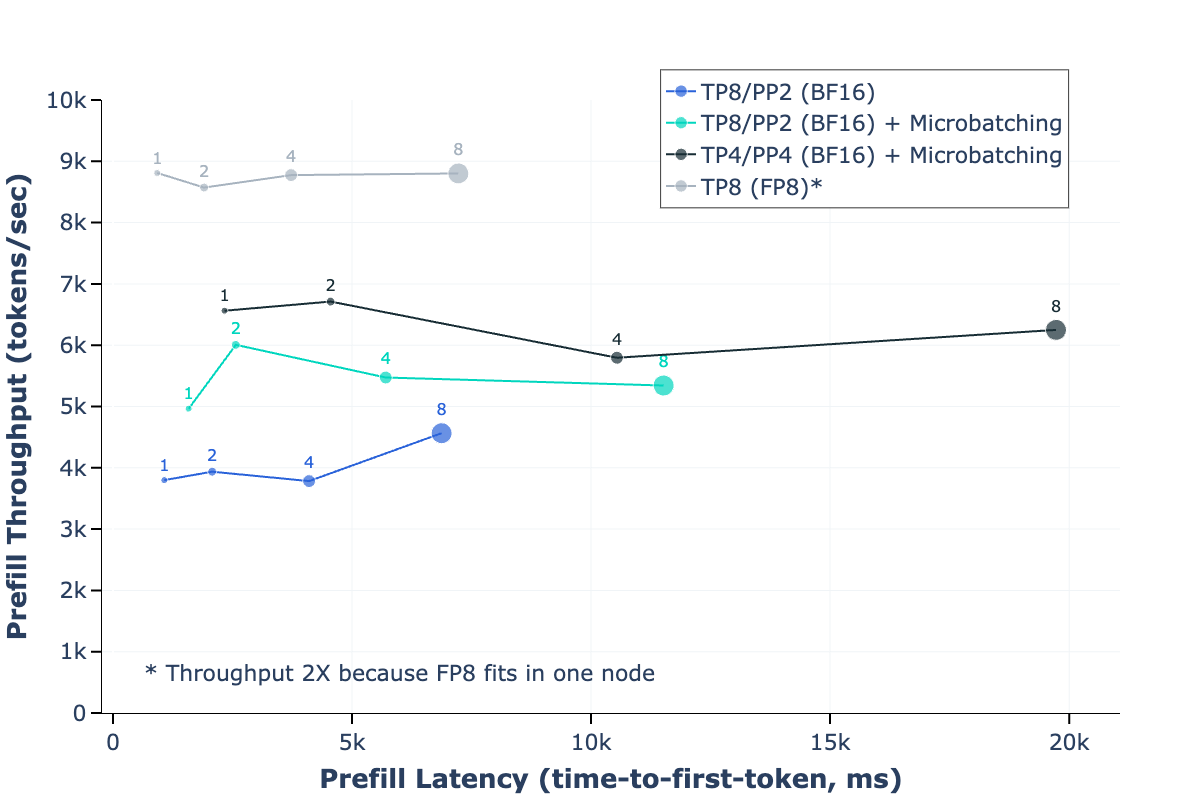
\includegraphics[width=\linewidth]{assets/prefill_fp8.png}
  \end{subfigure}%
  \begin{subfigure}{.5\textwidth}
    \centering
    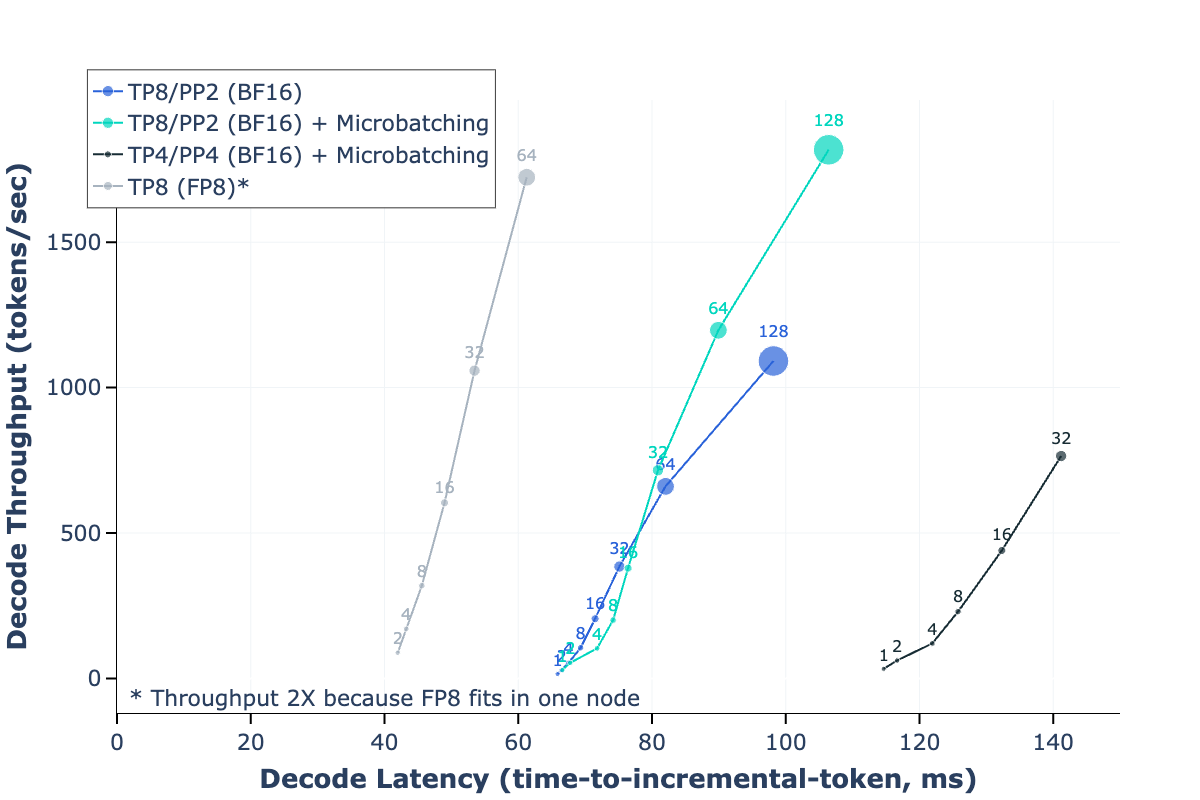
\includegraphics[width=\linewidth]{assets/decode_fp8.png}
  \end{subfigure}
  \caption{\textbf{Throughput-latency trade-off in FP8 inference with Llama 3 405B} compared with BF16 inference using different pipeline parallelization setups. \emph{Left:} Results for pre-filling. \emph{Right:} Results for decoding.}
  \label{figure:fp8_speed}
\end{figure}


\begin{figure}[t]
    \centering
    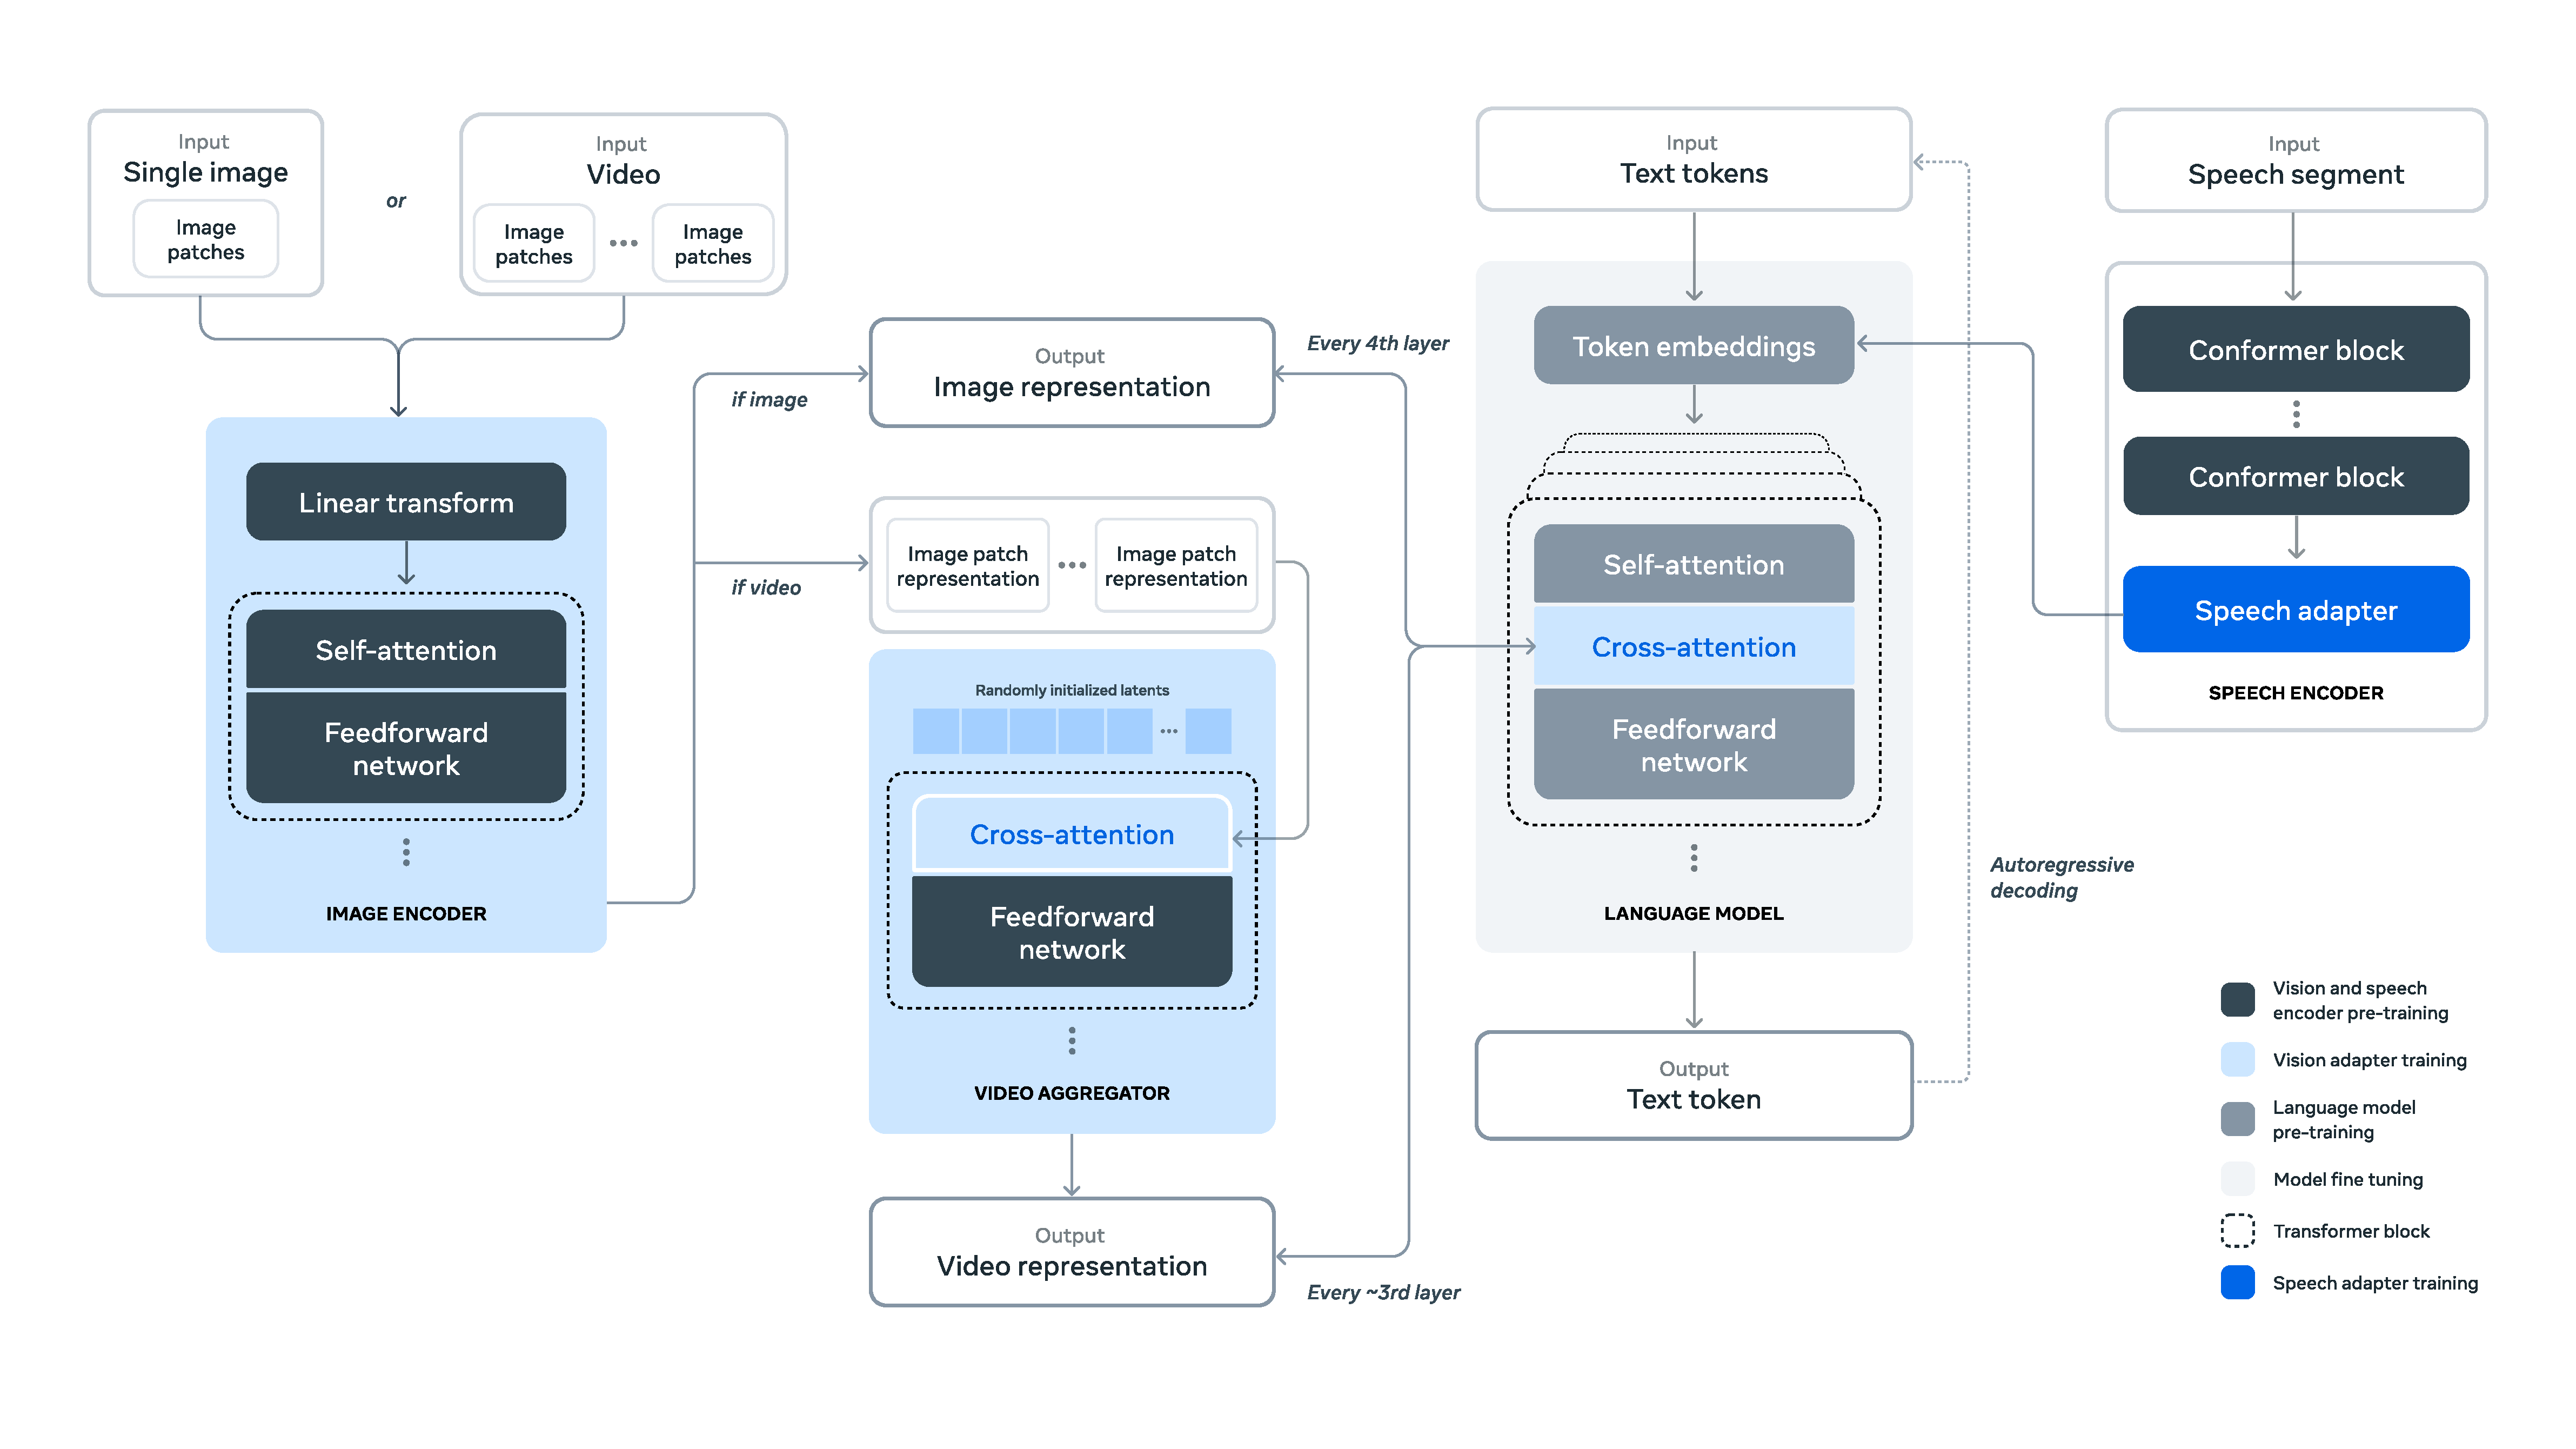
\includegraphics[width=\textwidth]{assets/llama3_architecture.pdf}
    \caption{\textbf{Illustration of the compositional approach to adding multimodal capabilities to Llama 3 that we study in this paper.} This approach leads to a multimodal model that is trained in five stages: \textbf{(1)} language model pre-training, \textbf{(2)} multi-modal encoder pre-training, \textbf{(3)} vision adapter training, \textbf{(4)} model finetuning, and \textbf{(5)} speech adapter training.}
    \label{sph:fig:multimodal_model_overview}
\end{figure}

\section{Vision Experiments}
\label{section:vision}

We perform a series of experiments in which we incorporate visual-recognition capabilities into \llamathree via a compositional approach that consists of two main stages.
First, we compose a pre-trained image encoder \citep{xu2023demystifying} and the pre-trained language model by introducing and training a set of cross-attention layers between the two models \citep{alayrac2022flamingo} on a large number of image-text pairs.
This leads to the model illustrated in Figure~\ref{sph:fig:multimodal_model_overview}.
Second, we introduce temporal aggregator layers and additional video cross-attention layers that operate on a large collection of video-text pairs to learn the model to recognize and process temporal information from videos.

A compositional approach to foundation model development has several advantages: \textbf{(1)} it enables us to parallelize the development of the vision and language modeling capabilities; \textbf{(2)} it circumvents complexities of joint pre-training on visual and language data that stem from tokenization of visual data, differences in background perplexities of tokens originating from different modalities, and contention between modalities; \textbf{(3)} it guarantees that model performance on text-only tasks is not affected by the introduction of visual-recognition capabilities, and \textbf{(4)} the cross-attention architecture ensures that we do not have to expend compute passing full-resolution images through the increasingly LLM backbones (specifically, the feed-forward networks in each transformer layer), making it more efficient during inference.
We note that our multimodal models are still under development and not yet ready for release.

Before presenting the results of our experiments in Section~\ref{section:results_image_recognition} and~\ref{section:results_video_recognition}, we describe the data we used to train visual recognition capabilities, the model architecture of the vision components, how we scale training of those components, and our pre-training and post-training recipes.

% \section{Center Embedding Leads to The Hierarchical Rule}
\section{Data Complexity Determines Rule Preference}
\label{sec:data_complexity}

We find that models generalize hierarchically because they are trained on data which includes center embeddings, a linguistic structure which we describe in Section \ref{sec:center_embed}. Center-embedded sentences drive hierarchical generalization in both the QF task (Section \ref{sec:qf_result}) and the TI task (Section \ref{sec:ti_result}).

\begin{figure}[t!]
    \centering
    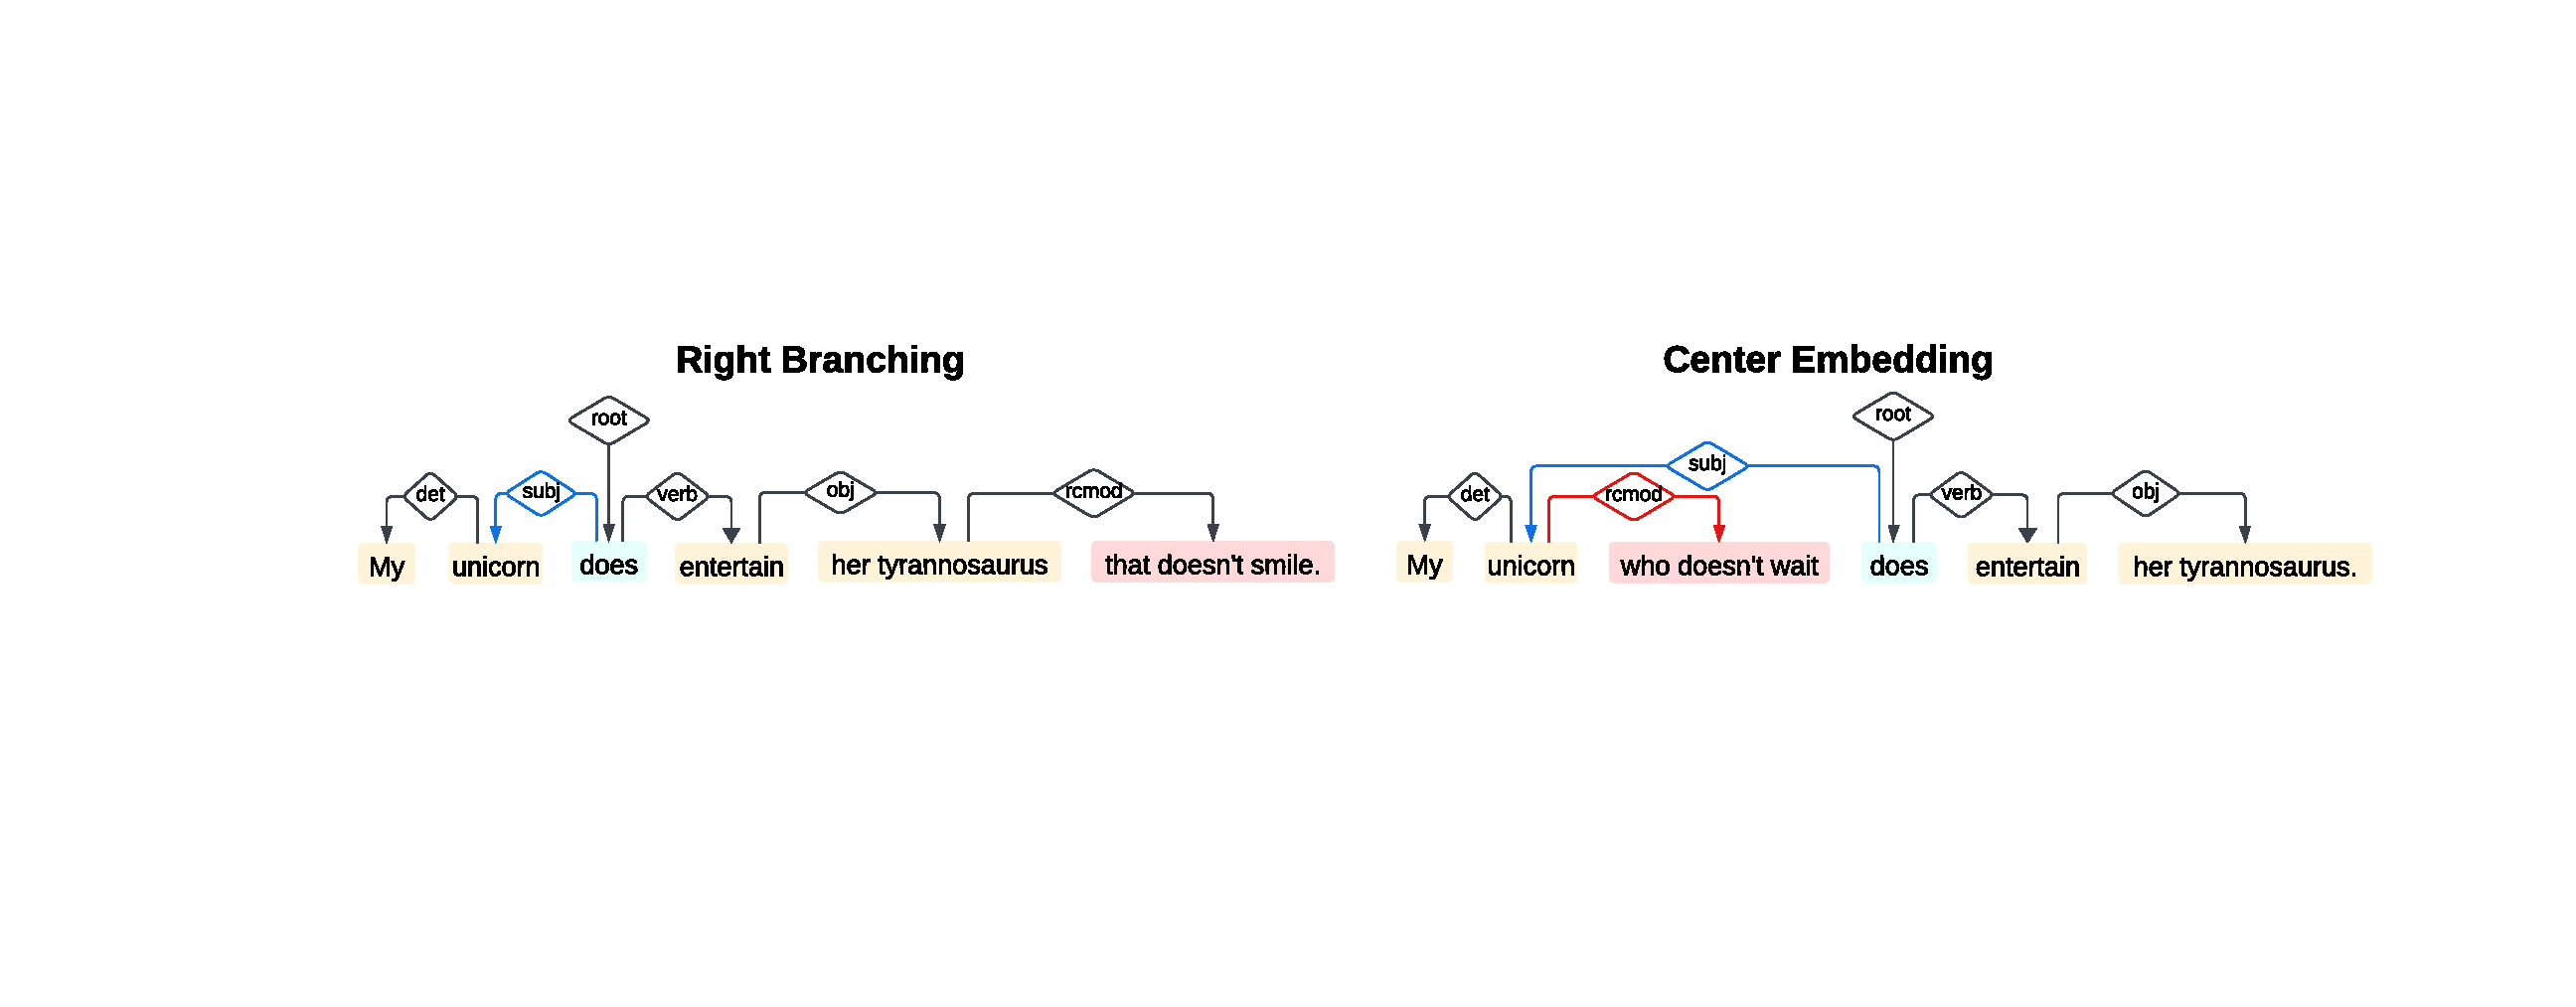
\includegraphics[width=1.0\textwidth]{figures/sentence_demo.pdf}
    \caption{\textbf{Sentence Examples.}   \textit{Left:} Right-branching sentence example. The linear progression of the main constituent is not interrupted by the relative clause. 
    \textit{Right:} Center-embedded sentence example. When the relative clause modifies the subject, it interrupts the linear progression of the main constituent. 
    }
    \label{fig:sentence_demo}
\end{figure}

\subsection{Center Embedding}
\label{sec:center_embed}
Center embedding occurs when a clause is placed recursively within another clause of the same type. Figure \ref{fig:sentence_demo} (\textit{left}) illustrates two examples of center-embedded sentences, where the embedded clause complicates syntactic parsing by placing an additional subject noun in between a verb and its own subject. Whereas center embeddings exhibit a recursive structure, sentences without center embeddings are exclusively right-branching. Right-branching structures may also include modifying clauses, but these clauses can only be appended at the end of the main clause, maintaining its linear flow (see Figure \ref{fig:sentence_demo}, \textit{right}). Linguists have long argued that center embeddings play a crucial role in grammar acquisition \citep{wexler1980formal} and give rise to tree-like syntactic structures \citep{Chomsky2015-bg}. 


We find that center embeddings, which are crucial for human language acquisition, also lead an LM to acquire hierarchical grammar rules. To correctly predict the next token, LMs must track syntactic connections between words in the context. In right-branching sentences, LMs can rely on linear proximity to identify these connections; as shown in Figure \ref{fig:sentence_demo}, a simple bigram model suffices to capture the subject-verb relationship for such sentences. In contrast, center embeddings introduce relative clauses of various lengths, making linear n-gram models inefficient for capturing subject-verb relationships. The recursive nature of the center embedding requires the model to track multiple subject-verb relationships: one for the main clause and a separate one for the embedded relative clause. In these cases, a tree structure is more efficient to model subject-verb relationships. 


\subsection{Question Formation Results}
\label{sec:qf_result}
As specified in Section \ref{sec:qf_task}, the training data for QF is ambiguous between the linear rule (i.e., moving the first auxiliary) and the hierarchical rule (i.e., moving the main auxiliary). Center-embedded sentences do not meet this ambiguity requirement and, therefore, cannot appear in question formation training samples. To ensure the model is exposed to diverse sentence types, \citet{McCoy2018-uv} introduced a secondary task to the QF training dataset: declaration copying. Like question formation, the declaration-copying example starts with a declarative sentence, but instead of transforming it, the model simply repeats it. Since the ambiguity requirement only applies to the primary question formation task, declaration-copying examples can include center embeddings. Concrete examples of both tasks can be found in Appendix \ref{appdx:data_sample}.


We train models on three modifications of the original training data, varying the composition of the declaration-copying subset. 
In \textit{Quest Only}, we remove all declaration-copying examples.
In \textit{Center embed}, we only keep center-embedded examples. In \textit{Right branch}, we only keep right-branching examples. 
Every modified training sets retains all examples of the primary task, question formation.
Every model trained, regardless of its training set composition, reaches 100\% in-distribution validation accuracy; however, the OOD generalization performance, shown in Figure \ref{fig:grokking_selection} (\textit{left}), differs significantly across the modified training sets. 

Our results confirm that declaration copying examples, specifically center embeddings, are essential for inducing hierarchical generalization.
Models trained without any declaration-copying examples fail to achieve an OOD accuracy above 75\%; so do models trained \textit{only} on right-branching  declaration-copying examples. When trained instead \textit{only} on center-embedded declaration-copying examples, models exhibit a strong preference for the hierarchical rule. This evidence suggests that center-embedded sentences direct a model towards the hierarchical rule. 

\begin{figure}[t!]
    \centering
    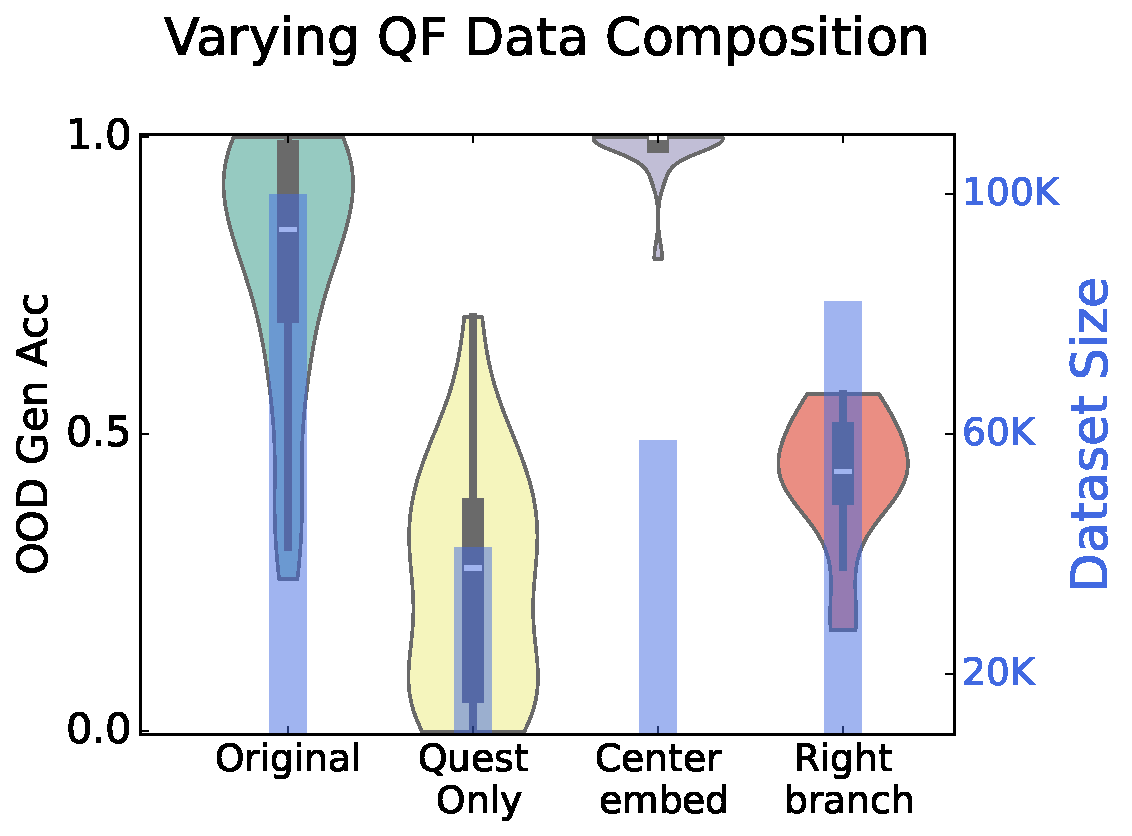
\includegraphics[width=0.41\linewidth]{figures/no_curriculum_main.pdf}
    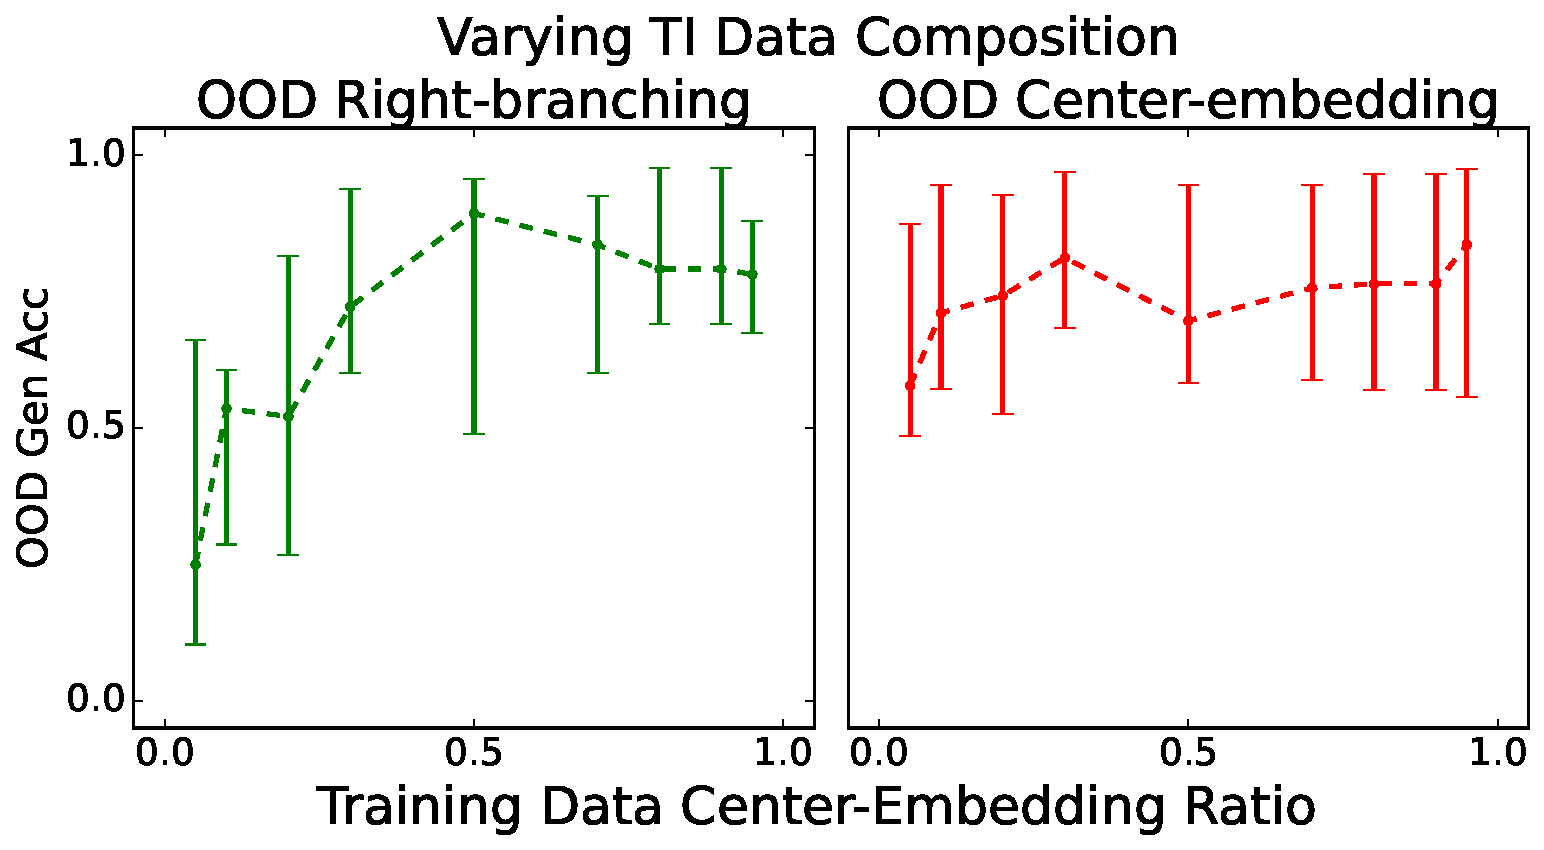
\includegraphics[width=0.55\linewidth]{figures/ti_simplicity_contamination.pdf}
    \caption{
    \textbf{Components of training data drive different generalization behaviors.} 
    \textit{Left:} Center-embedded sentences, which in the QF training data only appear in declaration copying examples, induce hierarchical generalization.
    \textit{Right:} Models are trained on different TI training data mixes and evaluated on two OOD sets: unambiguous right-branching sentences (\textit{green}) and unambiguous center-embedded sentences (\textit{red}). For center-embedded sentences, the hierarchical rule is preferred regardless of data mixes. For right-branching sentences, the model's preference for the hierarchical rule is exclusively driven by having a large mix of center-embedded sentences in the TI training data.}
    \label{fig:grokking_selection}
\end{figure}



\subsection{Tense Inflection Results}
\label{sec:ti_result}

In the TI training data, both right-branching and center-embedded sentences are made ambiguous by ensuring the distractor noun (i.e., a noun that appears between the main subject and the main verb) shares the same plurality as the main subject. For right-branching sentences, the distractor noun occurs in a prepositional phrase. For center-embedded sentences, the distractor noun occurs in a relative clause; either the subject or the object of the modifying clause can act as the distractor noun. We list examples below: 

\begin{enumerate}[itemsep=2pt,labelindent=10pt,topsep=0pt,parsep=0pt,partopsep=1pt, align=left, leftmargin=*]
    \item \textbf{Right Branching}: The noun in the prepositional phrase (e.g., `` \textit{to the cabinet}") acts as the distractor in the TI task.
    
    Example A (ID): \textit{The keys to the \textbf{cabinets} are on the table.}

    Example B (OOD): \textit{The keys to the \textbf{cabinet} are on the table.}
    
    \item \textbf{Center Embedding}: Either the subject or the object inside the relative clause acts as the distractor in the TI task.

    Example C (ID): \textit{The keys that unlock the \textbf{cabinets} are on the table.}

    Example D (OOD): \textit{The keys that unlock the \textbf{cabinet} are on the table.}
    
    
\end{enumerate}
We create variations of the TI training data by adjusting the ratio of right-branching to center-embedded samples while keeping the total training size constant.\footnote{The original training dataset contains a secondary past-tense copying task, to parallel the declaration-copying secondary task in QF. We show in Appendix \ref{appdx:ti_secondary} that the secondary task is not necessary, and we do not include it in our modified training sets.} A model's generalization behavior is tested on two OOD sets: one containing unambiguous right-branching sentences (e.g., Example B) and the other containing unambiguous center-embedded sentences (e.g., Example D). 

Generalization accuracies are shown in Figure \ref{fig:grokking_selection} (\textit{right}). When the training data is dominated by ambiguous right-branching sentences, the model fails to learn the hierarchical rule, as indicated by low OOD accuracy. However, when trained on a greater proportion of center-embedded sentences, the model systematically applies the hierarchical rule to both right-branching and center-embedded OOD sentences. As shown in Figure \ref{fig:grokking_selection} (\textit{right}), regardless of its training data mix, the model  generalizes hierarchically to OOD \textit{center embeddings}. In contrast, the model only generalizes hierarchically to \textit{right-branching sentences} after being exposed to a sufficient quantity of center-embedded sentences during training. In other words, the model eventually learns to treat non-recursive sequences as hierarchical through exposure to recursive center embeddings. These observations suggest that center embeddings drive the model's overall preference for tree structures. For further analysis of which center embedding structures induce this bias most efficiently, see Appendix \ref{appdx:obj_sbj_ctr_breakdown}.

% %%%%%%%%%%%%%%%%Previous version to preserve comments %%%%%%%%%%%%%%%%%%%%%%%%%%%%%%%%%%%%%%%%
% \iffalse
% \subsection{Tense Inflection} 
% \label{sec:ti_result}
% We now analyze hierarchical generalization in the tense inflection task, demonstrating the generality of our findings across grammatical rules. 
% The tense inflection setting from \citet{Linzen2016-vx} uses the same generation process as the question formation task, changing only the task itself.  
% This generation process leads to three types of sentences:

% \begin{enumerate}[itemsep=2pt,labelindent=10pt,topsep=0pt,parsep=0pt,partopsep=1pt, align=left, leftmargin=*]
%     \item The main verb immediately follows the subject noun.

%     Example: \textit{The keys are on the table.}
%     \item The main verb and the subject noun are separated by a prepositional phrase (e.g., `` \textit{to the cabinet}"). In all sentence examples, the prepositional phrase consistently follows the same syntactical structure and length (i.e., ``preposition $+$ determiner $+$ noun"). 

%     Example: \textit{The keys to the cabinet are on the table.}
%     \item The main verb and subject noun are separated by a relative clause, which can vary in syntactic composition and length.

%     Example: \textit{The keys that I used to unlock the cabinet are on the table.}
% \end{enumerate}


% By definition, both the first and second sentence types are right branching. In the second type, although a prepositional phrase is inserted within the main clause, it differs syntactically from a relative clause modifier. Unlike relative clause modifiers, prepositional phrases lack syntactic diversity, whereas relative clauses can exhibit the same of diversity as an entire sentence. In QF and TI data generated by CFG rules, a 4-gram model suffices to capture the subject-verb agreement. In contrast, relative clause modifiers (i.e., the third type) vary in both length and syntactic structure. All three sentence types are present in the original training data. Since sentences of the first type lack a distractor noun, they cannot be used to probe the model’s generalization, so the generalization set includes only the second and third types. As specified in Section \ref{sec:ti_task}, the TI training data only requires that the subject and distractor have the same plurality. Thus, center-embedded sentences can be included in the TI training data without violating the ambiguity requirement, and a secondary task is not necessary for TI.\footnote{In Appendix \ref{appdx:tense_tv}, we show that we can again leverage a secondary task such that a model trained on center-embedded tense inflection examples can generalize to right-branching sentences without having seen any examples of tense inflection on the sentence type, but not vice versa. }


% Our goal is to verify that center embeddings also drive OOD generalization in tense inflection. We create variations of the TI training data by adjusting the ratio of right-branching to center-embedded sentences, keeping the total training size constant. In Figure \ref{fig:ti_selection}, we report the model's OOD behavior across two data partitions. Figure \ref{fig:ti_selection} (\textit{left}) shows the model's generalization accuracy on unambiguous right-branching sentences when trained on different data mixes. When training data is dominated by ambiguous right-branching sentences, the model fails to learn the hierarchical rule, as indicated by low OOD generalization accuracy. However, as we increase the proportion of center-embedded sentences, these sentences---despite being ambiguous---bias the model towards the hierarchical rule, reflected by improved generalization accuracy.

% Figure \ref{fig:ti_selection} (\textit{right}) shows that the model consistently prefers the hierarchical rule for center-embedded sentences, regardless of data composition. These results indicate that the model’s preference for the hierarchical rule is primarily driven by center-embedded sentences. Moreover, with a high proportion of center-embedded sentences in the training data, this hierarchical rule preference extends to right-branching sentences as well.


% \fi
\subsection{Model Architecture}
\label{section:vision_model_architecture}
Our visual-recognition model consists of three main components: \textbf{(1)} an image encoder, \textbf{(2)} an image adapter, and \textbf{(3)} a video adapter.

\textbf{Image encoder.} Our image encoder is a standard vision transformer (ViT; \citet{dosovitskiy2020vit}) that is trained to align images and text \citep{xu2023demystifying}.
We use the ViT-H/14 variant of the image encoder, which has 630M parameters that were trained on 2.5B image-text pairs for five epochs.
The image encoder is pre-trained on images with resolution $224 \times 224$; images were split up into $16 \times 16$ patches of equal size (\emph{i.e.}, a patch size of $14x14$ pixels).
As also demonstrated by prior work such as ViP-Llava \citep{cai2023vipllava}, we observe that image encoders trained via a contrastive text alignment objective are unable to preserve fine-grained localization information. To alleviate this, we employ a \emph{multi-layer} feature extraction, where features from the \emph{4$^{th}$, 8$^{th}$, 16$^{th}$, 24$^{th}$ and 31$^{st}$} layers are also provided in addition to the final layer features.
In addition, we further insert 8 \emph{gated} self-attention layers (making a total of 40 transformer blocks) prior to pre-training of the cross-attention layers to learn alignment-specific features. The image encoder therefore eventually has a total $850$M parameters with the additional layers.
With the multi-layer features, the image encoder produces a $7680$-dimensional representation for each of the resulting $16 \times 16\!=\!256$ patches.
The parameters of the image encoder are \emph{not} frozen during subsequent training stages as we found it to improve performance, especially in domains such as text recognition.

\textbf{Image adapter.} We introduce cross-attention layers between the visual token representations produced by the image encoder and the token representations produced by the language model \citep{alayrac2022flamingo}.
The cross-attention layers are applied after every fourth self-attention layer in the core language model.
Like the language model itself, the cross-attention layers use generalized query attention (GQA) for increased efficiency.
The cross-attention layers introduce substantial numbers of additional trainable parameters into the model: for Llama 3 405B, the cross-attention layers have $\approx$100B parameters.
We pre-train our image adapter in two stages: (1) initial pre-training followed by (2) annealing:
\begin{itemize}
\item \textbf{Initial pre-training.} We pre-train our image adapter on our dataset of  $\sim$6B image-text pairs described above.
For compute efficiency reasons, we resize all images to fit within \emph{at most} four tiles of $336 \times 336$ pixels each, where we arrange the tiles to support different aspect ratios, \emph{e.g.}, $672 \times 672$, $672 \times 336$, and $1344 \times 336$.

\item \textbf{Annealing.}
We continue training the image adapter on $\sim$500M images from the annealing dataset described above.
During annealing, we increase the per-tile image resolution to improve performance on tasks that require higher-resolution images, for example, infographics understanding.
\end{itemize}

\textbf{Video adapter.} Our model takes as input up to 64 frames (uniformly sampled from a full video), each of which is processed by the image encoder.
We model temporal structure in videos through two components: \textbf{(i)} encoded video frames are aggregated by a temporal aggregator which merges 32 consecutive frames into one, \textbf{(ii)} additional video cross attention layers are added before every fourth image cross attention layer.
The temporal aggregator is implemented as a perceiver resampler~\citep{jaegle2021perceiver,alayrac2022flamingo}.
We pre-train using 16 frames per video (aggregated to 1 frame), but increase the number of input frames to 64 during supervised finetuning.
The video aggregator and cross attention layers have 0.6B and 4.6B parameters for Llama 3 7B and 70B, respectively. 




\newcommand{\cq}[1]{\textcolor{red}{\{CQ: #1\}}} %

\subsection{Infrastructure, Scaling, and Efficiency}
\label{section:pretraining_model_scaling}
We describe our hardware and infrastructure that powered \llamathree 405B pre-training at scale and discuss several optimizations that leads to improvements in training efficiency.

\subsubsection{Training Infrastructure}
The Llama 1 and 2 models were trained on Meta's AI Research SuperCluster~\citep{Lee22RSC}. As we scaled further, the training for Llama 3 was migrated to Meta's production clusters~\citep{lee2024building}.%
This setup optimizes for production-grade reliability, which is essential as we scale up training.

\textbf{Compute.}
\llamathree 405B is trained on up to 16K H100 GPUs, each running at 700W TDP with 80GB HBM3, using Meta's Grand Teton AI server platform~\citep{various2022grandteton}. Each server is equipped with eight GPUs and two CPUs. Within a server, the eight GPUs are connected via NVLink. Training jobs are scheduled using MAST~\citep{choudhury2024mast}, Meta's global-scale training scheduler.

\textbf{Storage.} 
Tectonic~\citep{pan2021tectonicfs}, Meta's general-purpose distributed file system, is used to build a storage fabric~\citep{battey2024storage} for Llama 3 pre-training. It offers 240 PB of storage out of 7,500 servers equipped with SSDs, and supports a sustainable throughput of 2 TB/s and a peak throughput of 7 TB/s. A major challenge is supporting the highly bursty checkpoint writes that saturate the storage fabric for short durations. Checkpointing saves each GPU’s model state, ranging from 1 MB to 4 GB per GPU, for recovery and debugging. We aim to minimize GPU pause time during checkpointing and increase checkpoint frequency to reduce the amount of lost work after a recovery. 

\textbf{Network.}
Llama 3 405B used RDMA over Converged Ethernet (RoCE) fabric based on the Arista 7800 and Minipack2 Open Compute Project\footnote{Open Compute Project: \url{https://www.opencompute.org/}} OCP rack switches. Smaller models in the Llama 3 family were trained using Nvidia Quantum2 Infiniband fabric. Both RoCE and Infiniband clusters leverage 400 Gbps interconnects between GPUs.  Despite the underlying network technology differences between these clusters, we tune both of them to provide equivalent performance for these large training workloads. We elaborate further on our RoCE network since we fully own its design.
\begin{itemize}

    \item \textbf{Network topology.} Our RoCE-based AI cluster comprises 24K GPUs\footnote{Note that we use only up to 16K of these 24K GPUs for Llama 3 pre-training.} connected by a three-layer Clos network~\citep{lee2024building}. At the bottom layer, each rack hosts 16 GPUs split between two servers and connected by a single Minipack2 top-of-the-rack (ToR) switch. In the middle layer, 192 such racks are connected by Cluster Switches to form a pod of 3,072 GPUs with full bisection bandwidth, ensuring no oversubscription. At the top layer, eight such pods within the same datacenter building are connected via Aggregation Switches to form a cluster of 24K GPUs. However, network connectivity at the aggregation layer does not maintain full bisection bandwidth and instead has an oversubscription ratio of 1:7. Our model parallelism methods (see Section~\ref{section:4D-parallelism}) and training job scheduler~\citep{choudhury2024mast} are all optimized to be aware of network topology, aiming to minimize network communication across pods.
    
    \item \textbf{Load balancing.} LLM training produces fat network flows that are hard to load balance across all available network paths using traditional methods such as Equal-Cost Multi-Path (ECMP) routing. To address this challenge, we employ two techniques. First, our collective library creates 16 network flows between two GPUs, instead of just one, thereby reducing the traffic per flow and providing more flows for load balancing. Second, our Enhanced-ECMP (E-ECMP) protocol effectively balances these 16 flows across different network paths by hashing on additional fields in the RoCE header of packets.
    
    \item \textbf{Congestion control.} We use deep-buffer switches in the spine~\citep{gangidi2024rmda} to accommodate transient congestion and buffering caused by collective communication patterns. This setup helps limit the impact of persistent congestion and network back pressure caused by slow servers, which is common in  training. Finally, better load balancing through E-ECMP significantly reduces the chance of congestion. With these optimizations, we successfully run a 24K GPU cluster without traditional congestion control methods such as Data Center Quantized Congestion Notification (DCQCN). 
\end{itemize}


\subsubsection{Parallelism for Model Scaling}
\label{section:4D-parallelism}

To scale training for our largest models, we use 4D parallelism—a combination of four different types of parallelism methods—to shard the model. This approach efficiently distributes computation across many GPUs and ensures each GPU's model parameters, optimizer states, gradients, and activations fit in its HBM. Our implementation of 4D parallelism is illustrated in Figure~\ref{fig:4d_parallelism}. It combines tensor parallelism (TP; \citet{NIPS2012_c399862d, shoeybi2019megatron, korthikanti2023reducing}), pipeline parallelism (PP; \citet{huang2019gpipe, narayanan2021efficient, lamy2023breadth}), context parallelism (CP; \citet{liu2023ring}), and data parallelism (DP; \citet{rajbhandari2020zeromemoryoptimizationstraining, ren2021zerooffloaddemocratizingbillionscalemodel, zhao2023pytorch}).

Tensor parallelism splits individual weight tensors into multiple chunks on different devices. Pipeline parallelism partitions the model vertically into stages by layers, so that different devices can process in parallel different stages of the full model pipeline. Context parallelism divides the input context into segments, reducing memory bottleneck for very long sequence length inputs. We use fully sharded data parallelism \citep[FSDP;][]{rajbhandari2020zeromemoryoptimizationstraining, ren2021zerooffloaddemocratizingbillionscalemodel, zhao2023pytorch}, which shards the model, optimizer, and gradients while implementing data parallelism which processes data in parallel on multiple GPUs and synchronizes after each training step. Our use of FSDP for Llama 3 shards optimizer states and gradients, but for model shards we do not reshard after forward computation to avoid an extra \texttt{all-gather} communication during backward passes.

\textbf{GPU utilization.}
Through careful tuning of the parallelism configuration, hardware, and software, we achieve an overall BF16 Model FLOPs Utilization (MFU; \citet{chowdhery2023palm}) of 38-43\% for the configurations shown in Table~\ref{table:mfu}.  The slight drop in MFU to 41\% on 16K GPUs with DP=128 compared to 43\% on 8K GPUs with DP=64 is due to the lower batch size per DP group needed to keep the global tokens per batch constant during training.

\begin{table}
	\centering
	\begin{tabular}{cccccccc|cc}
	\toprule
	     \textbf{GPUs} & \textbf{TP} & \textbf{CP} & \textbf{PP} & \textbf{DP}   & \textbf{Seq. Len.} &   \textbf{Batch size/DP} & \textbf{Tokens/Batch} & \textbf{TFLOPs/GPU} & \textbf{BF16 MFU}\\ 
	\midrule
	8,192    & 8 & 1 & 16 & 64   & 8,192   &   32 & 16M  & 430      & 43\%        \\
	16,384   & 8 & 1 & 16 & 128   & 8,192   &   16 & 16M  & 400      & 41\%        \\
	16,384   & 8 & 16 & 16 & 8   & 131,072 &   16 & 16M   & 380     & 38\%        \\
	\bottomrule

	\end{tabular}
\caption{\textbf{Scaling configurations and MFU for each stage of \llamathree 405B pre-training.} See text and Figure \ref{fig:4d_parallelism} for descriptions of each type of parallelism.}
\label{table:mfu}
\end{table}

\begin{figure}[t]
     \centering
     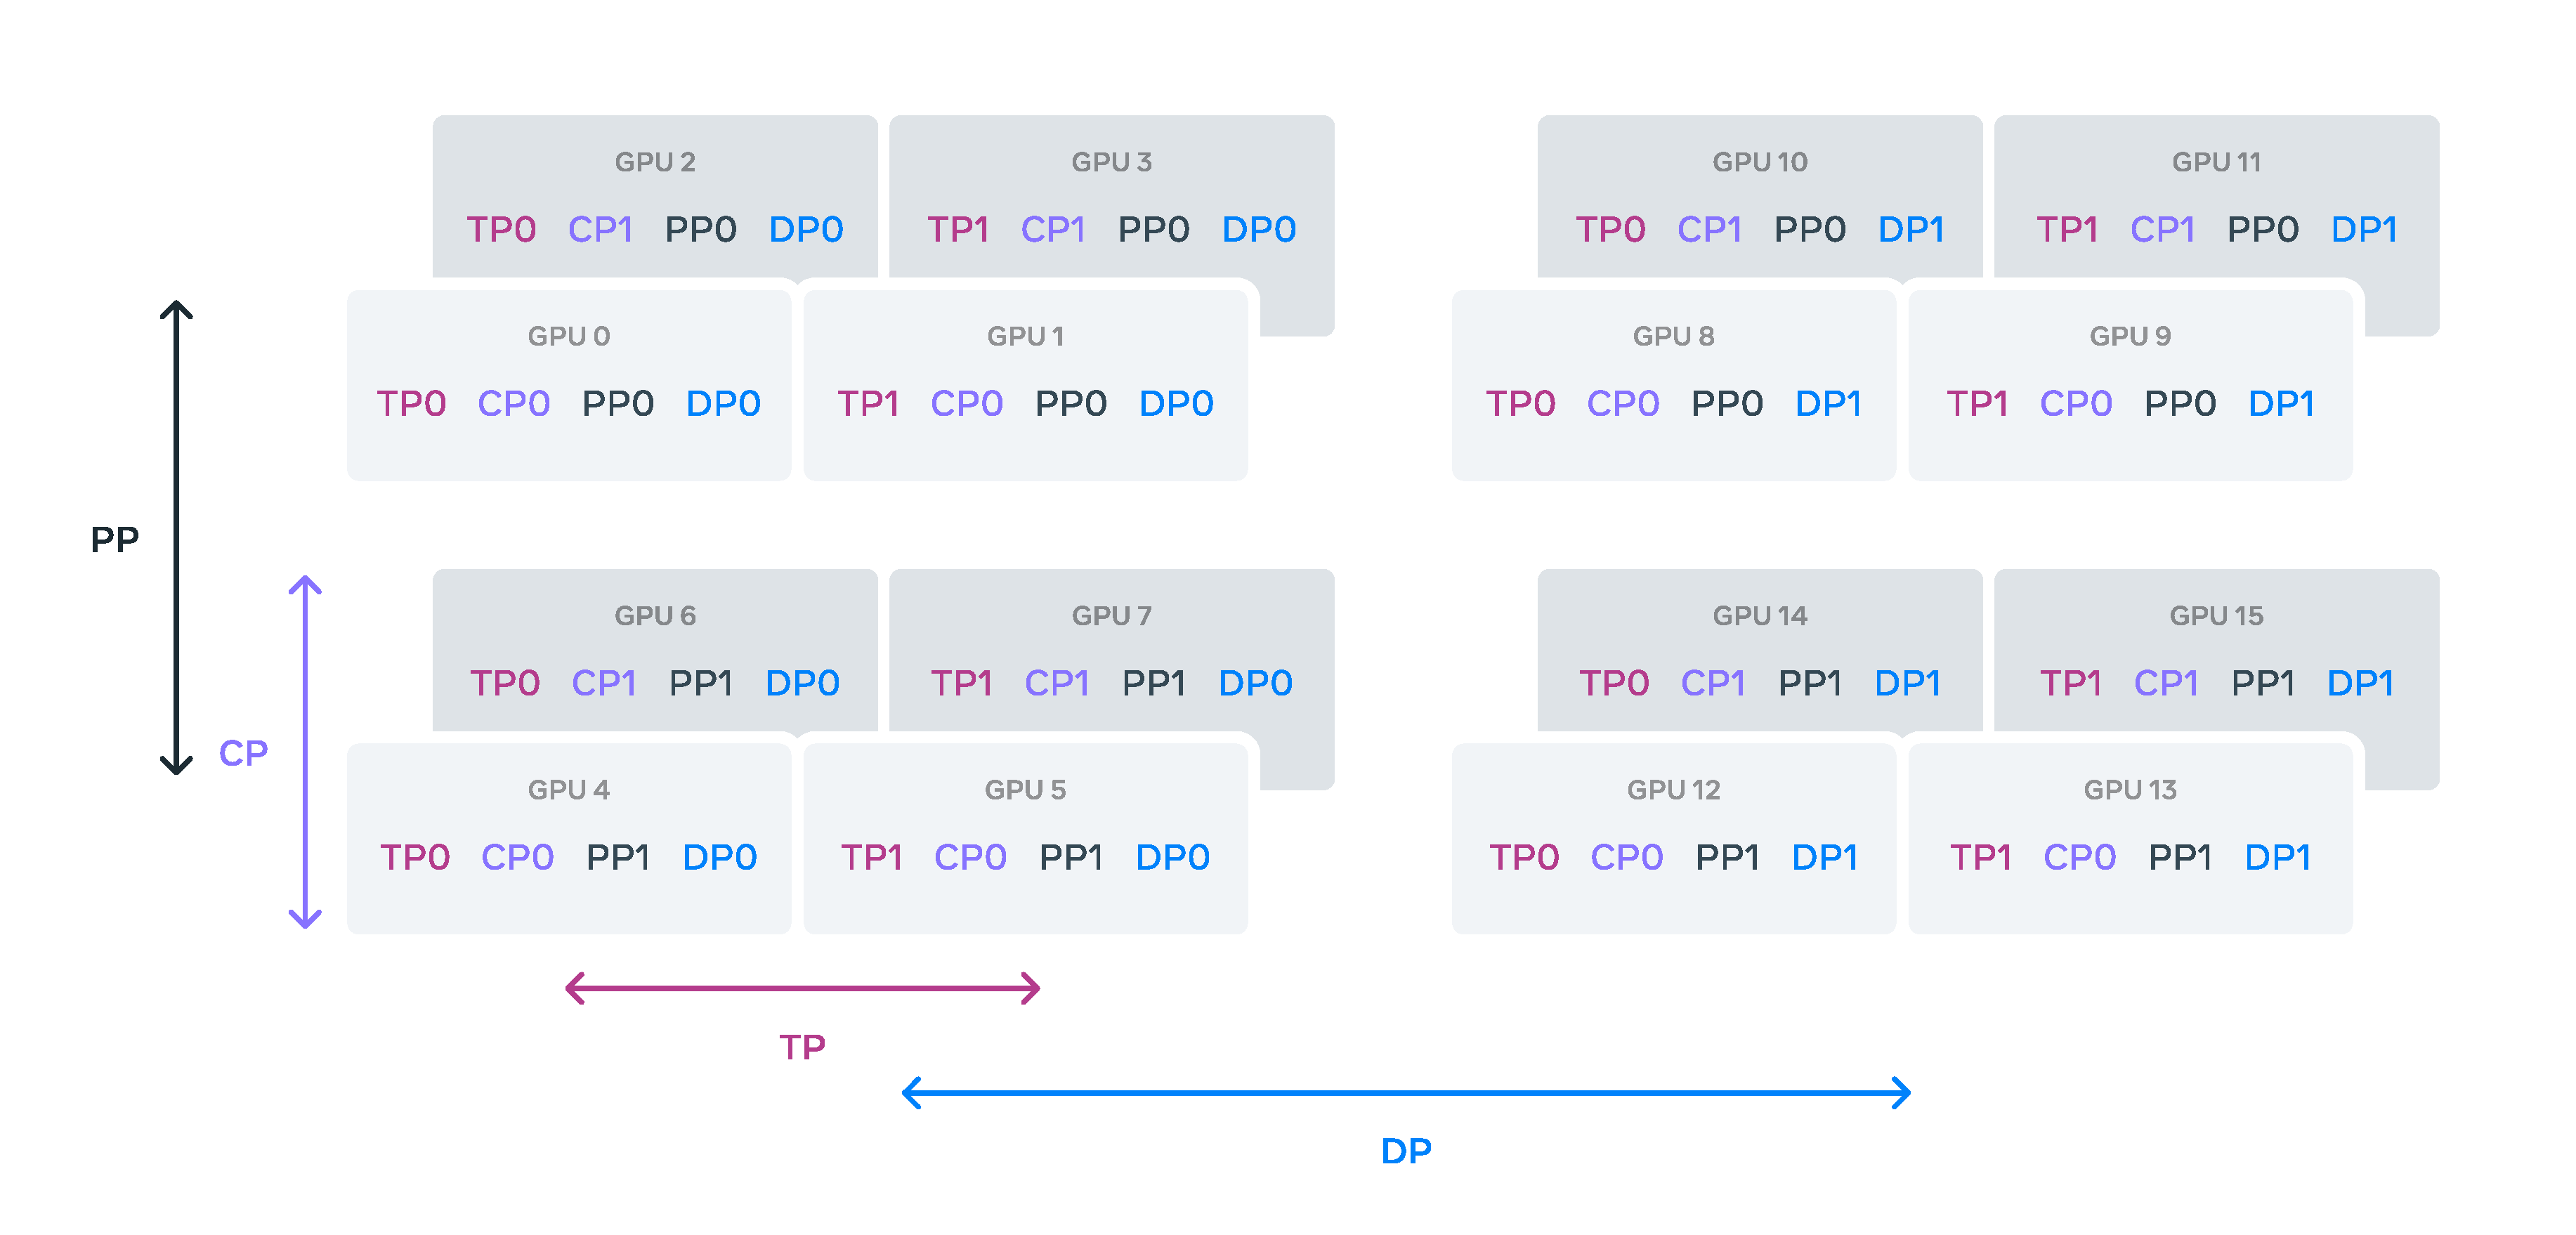
\includegraphics[width=\textwidth]{assets/4D_parallelism.pdf}
     \caption{\textbf{Illustration of 4D parallelism.} GPUs are divided into parallelism groups in the order of [TP, CP, PP, DP], where DP stands for FSDP. In this example, 16 GPUs are configured with a group size of |TP|=2, |CP|=2, |PP|=2, and |DP|=2. 
     A GPU's position in 4D parallelism is represented as a vector, [$D_1$, $D_2$, $D_3$, $D_4$], where $D_i$ is the index on the $i$-th parallelism dimension. In this example,
     GPU0[TP0, CP0, PP0, DP0] and GPU1[TP1, CP0, PP0, DP0] are in the same TP group, GPU0 and GPU2 are in the same CP group, GPU0 and GPU4 are in the same PP group, and GPU0 and GPU8 are in the same DP group.
     }
     \label{fig:4d_parallelism}
\end{figure}

\textbf{Pipeline parallelism improvements.}
We encountered several challenges with existing implementations:

\begin{itemize}
    \item \textbf{Batch size constraint.} Current implementations have constraints on supported batch size per GPU, requiring it to be divisible by the number of pipeline stages. For the example in Figure~\ref{fig:pipeline_parallelism}, the depth-first schedule (DFS) of pipeline parallelism~\citep{narayanan2021efficient} requires $N=\textrm{PP}=4$, while the breadth-first schedule (BFS; \citet{lamy2023breadth}) requires $N=M$, where $M$ is the total number of micro-batches and $N$ is the number of contiguous micro-batches for the same stage's forward or backward. However, pre-training often needs flexibility to adjust batch size.
    
    \item \textbf{Memory imbalance.} Existing pipeline parallelism implementations lead to imbalanced resource consumption. The first stage consumes more memory due to the embedding and the warm-up micro-batches.
    
    \item \textbf{Computation imbalance.} After the last layer of the model, we need to calculate output and loss, making this stage the execution latency bottleneck.
\end{itemize} 

To address these issues, we modify our pipeline schedule as shown in Figure~\ref{fig:pipeline_parallelism}, which allows setting $N$ flexibly---in this case $N=5$, which can run a arbitrary number of micro-batches in each batch. This allows us to run: (1) fewer micro-batches than the number of stages when we have batch size limit at large scale; or (2) more micro-batches to hide point-to-point communication, finding a sweet spot between DFS and breadth first schedule (BFS) for the best communication and memory efficiency. To balance the pipeline, we reduce one Transformer layer each from the first and the last stages, respectively. This means that the first model chunk on the first stage has only the embedding, and the last model chunk on the last stage has only output projection and loss calculation. To reduce pipeline bubbles, we use an interleaved schedule \citep{narayanan2021efficient} with $V$ pipeline stages on one pipeline rank. Overall pipeline bubble ratio is $\frac{\textrm{PP} - 1}{V * M}$. Further, we adopt asynchronous point-to-point communication in PP, which considerably speeds up training, especially in cases when the document mask introduces extra computation imbalance. We enable {\small \texttt{TORCH\_NCCL\_AVOID\_RECORD\_STREAMS}} to reduce memory usage from asynchronous point-to-point communication. Finally, to reduce memory cost, based on detailed memory allocation profiling, we proactively deallocate tensors that will not be used for future computation, including the input and output tensors of each pipeline stage, that will not be used for future computation. With these optimizations, we could pre-train \llamathree on sequences of 8K tokens without activation checkpointing.

\begin{figure*}[t]
     \centering
     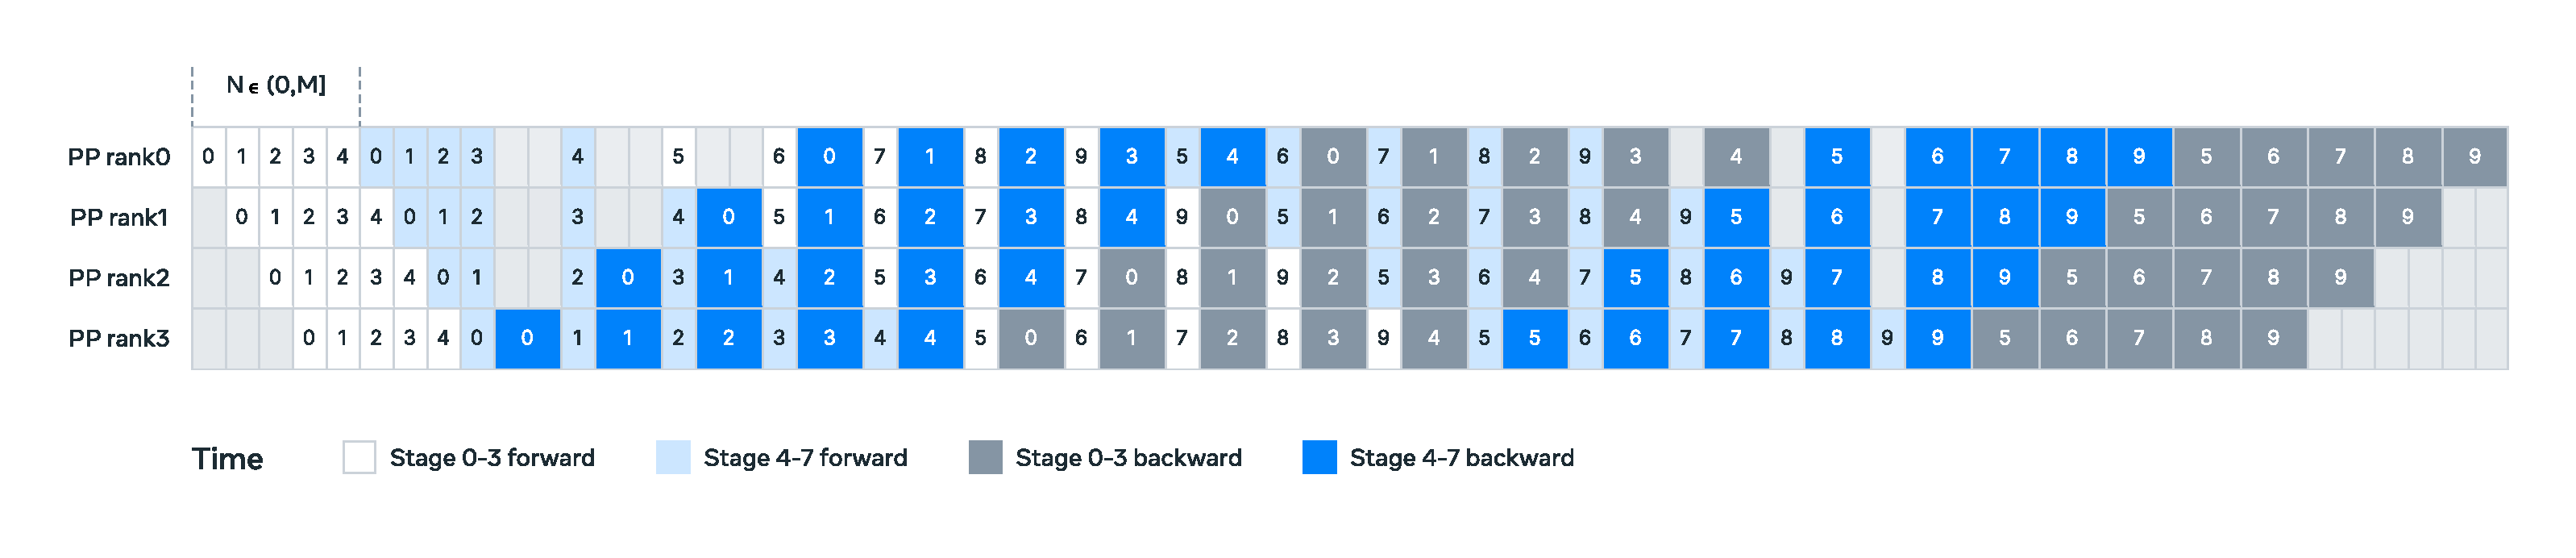
\includegraphics[width=\textwidth]{assets/pipeline_parallelism.pdf}
     \caption{\textbf{Illustration of pipeline parallelism in Llama 3.} Pipeline parallelism partitions eight pipeline stages (0 to 7) across four pipeline ranks (PP ranks 0 to 3), where the GPUs with rank 0 run stages 0 and 4, the GPUs with P rank 1 run stages 1 and 5, \emph{etc}. The colored blocks (0 to 9) represent a sequence of micro-batches, where $M$ is the total number of micro-batches and $N$ is the number of continuous micro-batches for the same stage's forward or backward. Our key insight is to make $N$ tunable.
     }
     \label{fig:pipeline_parallelism}
\end{figure*}

\textbf{Context parallelism for long sequences.} We utilize context parallelism (CP) to improve memory efficiency when scaling the context length of \llamathree and enable training on extremely long sequences up to 128K in length. In CP, we partition across the sequence dimension, and specifically we partition the input sequence into $2 \times \mbox{CP}$ chunks so each CP rank receives two chunks for better load balancing. The $i$-th CP rank received both the $i$-th and the $(2 \times \mbox{CP} - 1 - i)$-th chunks. 

Different from existing CP implementations that overlap communication and computation in a ring-like structure~\citep{liu2023ring}, our CP implementation adopts an \texttt{all-gather} based method where we first \texttt{all-gather} the key (K) and value (V) tensors, and then compute attention output for the local query (Q) tensor chunk. Although the \texttt{all-gather} communication latency is exposed in the critical path, we still adopt this approach for two main reasons: (1) it is easier and more flexible to support different types of attention masks in \texttt{all-gather} based CP attention, such as the document mask; and (2) the exposed \texttt{all-gather} latency is small as the communicated K and V tensors are much smaller than Q tensor due to the use of GQA \citep{ainslie2023gqa}. Hence, the time complexity of attention computation is an order of magnitude larger than \texttt{all-gather} ($O(S^2)$ versus $O(S)$, where $S$ represents the sequence length in the full causal mask), making the \texttt{all-gather} overhead negligible.

\textbf{Network-aware parallelism configuration.} The order of parallelism dimensions, [TP, CP, PP, DP], is optimized for network communication. The innermost parallelism requires the highest network bandwidth and lowest latency, and hence is usually constrained to within the same server. The outermost parallelism may spread across a multi-hop network and should tolerate higher network latency. Therefore, based on the requirements for network bandwidth and latency, we place parallelism dimensions in the order of [TP, CP, PP, DP]. DP (\emph{i.e.}, FSDP) is the outermost parallelism because it can tolerate longer network latency by asynchronously prefetching sharded model weights and reducing gradients. Identifying the optimal parallelism configuration with minimal communication overhead while avoiding GPU memory overflow is challenging. We develop a memory consumption estimator and a performance-projection tool which helped us explore various parallelism configurations and project overall training performance and identify memory gaps effectively.

\textbf{Numerical stability.} By comparing training loss between different parallelism setups, we fixed several numerical issues that impact training stability. To ensure training convergence, we use FP32 gradient accumulation during backward computation over multiple micro-batches and also \texttt{reduce-scatter} gradients in FP32 across data parallel workers in FSDP. For intermediate tensors, \emph{e.g.}, vision encoder outputs, that are used multiple times in the forward computation, the backward gradients are also accumulated in FP32.

\subsubsection{Collective Communication}
\label{sec:ncclx}

Our collective communication library for \llamathree is based on a fork of Nvidia's NCCL library, called NCCLX. NCCLX significantly improves the performance of NCCL, especially for higher latency networks. Recall that the order of parallelism dimensions is [TP, CP, PP, DP], where DP corresponds to FSDP. The outermost parallelism dimensions, PP and DP, may communicate through a multi-hop network, with latency up to tens of microseconds. The original NCCL collectives---\texttt{all-gather} and \texttt{reduce-scatter} in FSDP, and \texttt{point-to-point} in PP---require data chunking and staged data copy. This approach incurs several inefficiencies, including (1) requiring a large number of small control messages to be exchanged over the network to facilitate data transfer, (2) extra memory-copy operations, and (3) using extra GPU cycles for communication.  For \llamathree training, we address a subset of these inefficiencies by tuning chunking and data transfer to fit our network latencies, which can be as high as tens of microseconds for a large cluster. We also allow small control messages to traverse our network at a higher priority, especially avoiding being head-of-line blocked in deep-buffer core switches. Our ongoing work for future Llama versions involves making deeper changes in NCCLX to holistically address all the aforementioned problems.

\subsubsection{Reliability and Operational Challenges}

The complexity and potential failure scenarios of 16K GPU training surpass those of much larger CPU clusters that we have operated. Moreover, the synchronous nature of training makes it less fault-tolerant---a single GPU failure may require a restart of the entire job. Despite these challenges, for \llamathree, we achieved higher than 90\% effective training time while supporting automated cluster maintenance, such as firmware and Linux kernel upgrades~\citep{leonhardi2024maintenance}, which resulted in at least one~training interruption daily. The effective training time measures the time spent on useful training over the elapsed time.

During a 54-day snapshot period of pre-training, we experienced a total of 466 job interruptions. Of these, 47 were planned interruptions due to automated maintenance operations such as firmware upgrades or operator-initiated operations like configuration or dataset updates. The remaining 419 were unexpected interruptions, which are classified in Table~\ref{table:job_interruptions}.
Approximately 78\% of the unexpected interruptions are attributed to confirmed hardware issues, such as GPU or host component failures, or suspected hardware-related issues like silent data corruption and unplanned individual host maintenance events. GPU issues are the largest category, accounting for 58.7\% of all unexpected issues.  Despite the large number of failures, significant manual intervention was required only three times during this period, with the rest of issues handled by automation. 

\begin{table}[]
\centering
\begin{tabular}{lccc}
    \toprule
\textbf{Component}             & \textbf{Category} & \textbf{Interruption Count} & \textbf{\% of Interruptions} \\
\midrule
Faulty GPU                            & GPU               & 148                         & 30.1\%                       \\
GPU HBM3 Memory                & GPU               & 72                          & 17.2\%                       \\
Software Bug                   & Dependency          & 54                          & 12.9\%                       \\
Network Switch/Cable           & Network           & 35                          & 8.4\%                        \\
Host Maintenance               & \begin{tabular}[c]{@{}c@{}}Unplanned \\ Maintenance\end{tabular}       & 32                          & 7.6\%                        \\
GPU SRAM Memory                & GPU               & 19                          & 4.5\%                        \\
GPU System Processor           & GPU               & 17                          & 4.1\%                        \\
NIC                            & Host              & 7                           & 1.7\%                        \\
NCCL Watchdog Timeouts                  & Unknown           & 7                           & 1.7\%                        \\
Silent Data Corruption                      & GPU           & 6                           & 1.4\%                        \\
GPU Thermal Interface + Sensor & GPU               & 6                           & 1.4\%                        \\
SSD                            & Host              & 3                           & 0.7\%                        \\
Power Supply                   & Host              & 3                           & 0.7\%                        \\
Server Chassis                 & Host              & 2                           & 0.5\%                        \\
IO Expansion Board             & Host              & 2                           & 0.5\%                        \\
Dependency                     & Dependency        & 2                           & 0.5\%                        \\
CPU                            & Host              & 2                           & 0.5\%                        \\
System Memory                  & Host              & 2                           & 0.5\%    \\
\bottomrule
\end{tabular}
\caption{\textbf{Root-cause categorization of unexpected interruptions during a 54-day period of Llama 3 405B pre-training.} About 78\% of unexpected interruptions were attributed to confirmed or suspected hardware issues. }
\label{table:job_interruptions}
\end{table}

To increase the effective training time, we reduced job startup and checkpointing time, and developed tools for fast diagnosis and problem resolution. We extensively use PyTorch's built-in NCCL flight recorder~\citep{ansel2024pytorch}, a feature that captures collective metadata and stack traces into a ring buffer, and hence allowing us to diagnose hangs and performance issues quickly at scale, particularly with regard to NCCLX. Using this, we efficiently record every communication event and the duration of each collective operation, and also automatically dump tracing data on NCCLX watchdog or heartbeat timeout. We enable more computationally intensive tracing operations and metadata collection selectively as needed live in production through online configuration changes~\citep{configerator} without needing a code release or job restart.

Debugging issues in large-scale training is complicated by the mixed use of NVLink and RoCE in our network. Data transfer over NVLink typically occurs through load/store operations issued by CUDA kernels, and failures in either the remote GPU or NVLink connectivity often manifest as stalled load/store operations within CUDA kernels without returning a clear error code. NCCLX enhances the speed and accuracy of failure detection and localization through a tight co-design with PyTorch, allowing PyTorch to access NCCLX’s internal state and track relevant information. While stalls due to NVLink failures cannot be completely prevented, our system monitors the state of the communication library and automatically times out when such a stall is detected. Additionally, NCCLX traces the kernel and network activities of each NCCLX communication and provides a snapshot of the failing NCCLX collective's internal state, including finished and pending data transfers between all ranks. We analyze this data to debug NCCLX scaling issues.

Sometimes, hardware issues may cause still-functioning but slow stragglers that are hard to detect. Even a single straggler can slow down thousands of other GPUs, often appearing as functioning but slow communications. We developed tools to prioritize potentially problematic communications from selected process groups. By investigating just a few top suspects,  we were usually able to effectively identify the stragglers.

One interesting observation is the impact of environmental factors on training performance at scale. For Llama 3 405B , we noted a diurnal 1-2\% throughput variation based on time-of-day. This fluctuation is the result of higher mid-day temperatures impacting GPU dynamic voltage and frequency scaling.

During training, tens of thousands of GPUs may increase or decrease power consumption at the same time, for example, due to all GPUs waiting for checkpointing or collective communications to finish, or the startup or shutdown of the entire training job. When this happens, it can result in instant fluctuations of power consumption across the data center on the order of tens of megawatts, stretching the limits of the power grid. This is an ongoing challenge for us as we scale training for future, even larger Llama models.

\subsection{Pre-training}
\label{section:vision_training_recipe}

\textbf{Image.}
We initialize from the pre-trained text model and vision encoder weights.
The vision encoder is unfrozen, while the text model weights are kept frozen as explained above.
First, we train the model using 6B image-text pairs where each image is resized to fit within four tiles of $336 \times 336$ pixels.
We use a global batch size of 16,384 and a cosine learning rate schedule with initial learning rate $10 \times 10^{-4}$ and a weight decay of $0.01$.
The initial learning rate was determined based on small-scale experiments.
However,  these findings did not generalize well to very long training schedules and dropped the learning rate a few times during training when the loss values became stagnant.
After the base pre-training, we increase the image resolution further and continue training the same weights on the annealing dataset.
The optimizer is re-initialized via warm-up to learning rate $2 \times 10^{-5}$ and again follows a cosine schedule.

\textbf{Video.}
For video pre-training, we start from the image pre-trained and annealed weights as described above.
We add the video aggregator and cross-attention layers as described in the architecture, initialized randomly. We freeze all the parameters in the model except the video-specific ones (the aggregator and video cross-attention), and train them on the video pre-training data.
We use the same training hyperparameters as the image annealing stage, with small differences in the learning rate.
We uniformly sample 16 frames from the full video, and represent each frame using four chunks, each of size of $448 \times 448$ pixels.
We use an aggregation factor of 16 in the video aggregator, hence obtaining one effective frame, which the text tokens cross-attend to.
We use a global batch size of 4,096, a sequence length of 190 tokens, and a learning rate of $10^{-4}$ during training.

\subsection{Post-Training}
\label{section:vision_post_training}
In this section, we describe the post-training recipe for our vision adapters. After pre-training, we fine-tune the model on highly curated multi-modal conversational data to enable chat capabilities. We further implement direct preference optimization (DPO) to boost human evaluation performance and rejection sampling to improve multi-modal reasoning capabilities. Finally, we add a quality-tuning stage where we continue fine-tuning the model on a very small set of high-quality conversational data which further boosts human evaluation while retaining performance across benchmarks. More details on each of these steps are provided below.

\subsubsection{Supervised Finetuning Data}
\label{subsubsection:vision_supervised_finetuning_data}
We describe our supervised finetuning (SFT) data for image and video capabilities separately below.

\textbf{Image.} We utilize a mix of different datasets for supervised finetuning.
\begin{itemize}
\item \textbf{Academic datasets.} We convert a highly filtered collection of existing academic datasets to question-answer pairs using templates or via LLM rewriting. The LLM rewriting's purpose is to augment the data with different instructions and to improve the language quality of answers.

\item \textbf{Human annotations.} We collect multi-modal conversation data via human annotators for a wide range of tasks (open-ended question-answering, captioning, practical use cases, \textit{etc.}) and domains (\textit{e.g.}, natural images and structured images). Annotators are provided with images and asked to write conversations. To ensure diversity, we cluster large-scale datasets and sampled images uniformly across different clusters. Further, we acquire additional images for a few specific domains by expanding a seed via k-nearest neighbors. Annotators are also provided with intermediate checkpoints of existing models to facilitate model-in-the-loop style annotations, so that model generations can be utilized as a starting point by the annotators to then provide additional human edits. This is an iterative process, in which model checkpoints would be regularly updated with better performing versions trained on the latest data. This increases the volume and efficiency of human annotations, while also improving their quality.

\item \textbf{Synthetic data.} We explore different ways to generate synthetic multi-modal data by using text-representations of images and a text-input LLM. The high-level idea is to utilize the reasoning capabilities of text-input LLMs to generate question-answer pairs in the text domain, and replace the text representation with its corresponding images to produce synthetic multi-modal data. Examples include rendering texts from question-answer datasets as images or rendering table data into synthetic images of tables and charts. Additionally, we use captions and OCR extractions from existing images to generate additional conversational or question-answer data related to the images.
\end{itemize}

\textbf{Video.} Similar to the image adapter, we use academic datasets with pre-existing annotations and convert them into appropriate textual instructions and target responses.
The targets are converted to open-ended responses or multiple-choice options, whichever is more appropriate.
We ask humans to annotate videos with questions and corresponding answers.
The annotators are asked to focus on questions that could not be answered based on a single frame, to steer the annotators towards questions that require temporal understanding.

\subsubsection{Supervised Finetuning Recipe}
We describe our supervised finetuning (SFT) recipe for image and video capabilities separately below.

\label{subsubsection:vision_supervised_finetuning_recipe}
\textbf{Image.} We initialize from the pre-trained image adapter, but hot-swap the pre-trained language model's weights with the instruction tuned language model's weights. The language model weights are kept frozen to maintain text-only performance, \textit{i.e.}, we only update the vision encoder and image adapter weights.

Our approach to finetune the model is similar to \cite{wortsman2022modelsoupsaveragingweights}. First, we run a hyperparameter sweep using multiple random subsets of data, learning rates and weight decay values. Next, we rank the models based on their performance. Finally, we average the weights of the top-$K$ models to obtain the final model. The value of $K$ is determined by evaluating the averaged models and selecting the instance with highest performance. We observe that the averaged models consistently yield better results compared to the best individual model found via grid search. Further, this strategy reduces sensitivity to hyperparameters.

\textbf{Video.} For video SFT, we initialize the video aggregator and cross-attention layers using the pre-trained weights.
The rest of the parameters in the model, the image weights and the LLM, are initialized from corresponding models following their finetuning stages.
Similar to video pre-training, we then finetune only the video parameters on the video SFT data.
For this stage, we increase the video length to 64 frames, and use an aggregation factor of 32 to get two effective frames.
The resolution of the chunks is also increased to be consistent with the corresponding image hyperparameters.

\subsubsection{Preference Data}
\label{subsubsection:vision_preference_data}
We built multimodal pair-wise preference datasets for reward modeling and direct preference optimization.
\begin{itemize}

\item \textbf{Human annotations.} The human-annotated preference data consists of comparisons between two different model outputs, labeled as ``chosen'' and ``rejected'', with 7-scale ratings. The models used to generate responses are sampled on-the-fly from a pool of the best recent models, each with different characteristics. We update the model pool weekly. Besides preference labels, we also request annotators to provide optional human edits to correct inaccuracies in ``chosen'' responses because vision tasks have a low tolerance for inaccuracies. Note that human editing is an optional step because there is a trade-off between volume and quality in practice.

\item \textbf{Synthetic data.} Synthetic preference pairs could also be generated by using text-only LLMs to edit and deliberately introduce errors in the supervised finetuning dataset. We took the conversational data as input, and use an LLM to introduce subtle but meaningful errors (\textit{e.g.}, change objects, change attributes, add mistakes in calculations, etc.). These edited responses are used as negative ``rejected'' samples and paired with the ``chosen'' original supervised finetuning data.

\item \textbf{Rejection sampling.} Furthermore, to create more \emph{on-policy} negative samples, we leveraged the iterative process of rejection sampling to collect additional preference data. We discuss our usage of rejection sampling in more detail in the following sections. At a high-level, rejection sampling is used to iteratively sample high-quality generations from a model. Therefore, as a by-product, all generations that are not selected can be used as negative rejected samples and used as additional preference data pairs.

\end{itemize}

\subsubsection{Reward Modeling}
\label{subsubsection:vision_reward_modeling}
We train a vision reward model (RM) on top of the vision SFT model and the language RM. The vision encoder and the cross-attention layers are initialized from the vision SFT model and unfrozen during training, while the self-attention layers are initialized from the language RM and kept frozen. We observe that freezing the language RM part generally leads to better accuracy, especially on tasks that require the RM to judge based on its knowledge or the language quality. We adopt the same training objective as the language RM, but adding a weighted regularization term on the square of the reward logits averaged over the batch, which prevents the reward scores from drifting.

The human preference annotations in Section~\ref{subsubsection:vision_preference_data} are used to train the vision RM. We follow the same practice as language preference data (Section~\ref{sec:rlhf_annotation_data}) to create two or three pairs with clear ranking (\emph{edited} > \emph{chosen} > \emph{rejected}). In addition, we also synthetically augment the negative responses by perturbing the words or phrases related to the information in the image (such as numbers or visual texts). This encourages the vision RM to ground its judgement based on the actual image content.

\subsubsection{Direct Preference Optimization}
\label{subsubsec:dpo}
Similar to the language model (Section~\ref{subsubsec:postdpo}), we further train the vision adapters with Direct Preference Optimization (DPO;~\cite{rafailov2023dpo}) using the preference data described in Section~\ref{subsubsection:vision_preference_data}. To combat the distribution shift during post-training rounds, we only keep recent batches of human preference annotations while dropping batches that are sufficiently off-policy (\textit{e.g.}, if the base pre-trained model is changed). We find that instead of always freezing the reference model, updating it in an exponential moving average (EMA) fashion every k-steps helps the model learn more from the data, resulting in better performance in human evaluations. Overall, we observed that the vision DPO model consistently performs better than its SFT starting point in human evaluations for every finetuning iteration.

\subsubsection{Rejection Sampling}
\label{subsubsection:vision_rejection_sampling}
Most available question-answer pairs only contain the final answer and lack the chain-of-thought explanation that is required to train a model that generalizes well for reasoning tasks.
We use rejection sampling to generate the missing explanations for such examples and boost the model's reasoning capabilities.

Given a question-answer pair, we generate multiple answers by sampling the finetuned model with different system prompts or temperature.
Next, we compare the generated answers to the ground-truth via heuristics or an LLM judge.
Finally, we retrain the model by adding the correct answers back into the finetuning data mix. We find it useful to keep multiple correct answers per question.

To ensure we only add high-quality examples back into training, we implemented the following two guardrails.
First, we find that some examples contain incorrect explanations, despite the final answer being correct.
We observed that this pattern occurs more frequently for questions where only a small fraction of the generated answers is correct.
Therefore, we drop answers for questions where the probability of the answer being correct is below a certain threshold.
Second, raters prefer some answers over others due to differences in language or style.
We use the reward model to select top-$K$ highest-quality answers and add them back into training.

\subsubsection{Quality Tuning}
\label{subsubsection:vision_quality_tuning}
We curate a small but \emph{highly} selective SFT dataset where all samples have been rewritten and verified either by humans or our best models to meet our highest standards. We train DPO models with this data to improve response quality, calling the process Quality-Tuning (QT). We find that QT significantly improves human evaluations without affecting generalization verified by benchmarks when the QT dataset covers a wide range of tasks and proper early stopping is applied. We select checkpoints at this stage purely based on benchmarks to ensure capabilities are retained or improved.

\begin{NiceTabular}{lccccccc}
    \CodeBefore
    \Body
    \toprule
    & \textbf{Llama 3-V 8B} & \textbf{Llama 3-V 70B} & \textbf{Llama 3-V 405B} & \textbf{GPT-4V} & \textbf{GPT-4o} & \textbf{Gemini 1.5 Pro} & \textbf{Claude 3.5} \\
    \midrule
    MMMU \scriptsize{(val, CoT)} & 49.6 & 60.6 & 64.5 & 56.4 & \textbf{69.1} & 62.2 & 68.3 \\
    VQAv2 \scriptsize{(test-dev)} & 78.0 & 79.1 & \textbf{80.2} & 77.2 & -- & \textbf{80.2} & --\\
    AI2 Diagram \scriptsize{(test)} & 84.4 & 93.0 & 94.1 & 78.2 & 94.2 & 94.4 & \textbf{94.7} \\
    ChartQA \scriptsize{(test, CoT)} & 78.7 & 83.2 & 85.8 & 78.4 & 85.7 & 87.2 & \textbf{90.8} \\
    TextVQA \scriptsize{(val)} & 78.2 & 83.4 & \textbf{84.8} & 78.0 & -- & 78.7 & --\\
    DocVQA \scriptsize{(test)} & 84.4 & 92.2 & 92.6 & 88.4 & 92.8 & ~~93.1$^{\triangle}$ & \textbf{95.2} \\
    \bottomrule
\end{NiceTabular}

\begin{NiceTabular}{lccccccc}
    \CodeBefore
    \Body
    \toprule
    & \textbf{Llama 3-V 8B} & \textbf{Llama 3-V 70B} & \textbf{Gemini 1.0 Pro} & \textbf{Gemini 1.0 Ultra} & \textbf{Gemini 1.5 Pro} & \textbf{GPT-4V} & \textbf{GPT-4o} \\
    \midrule
    PerceptionTest \scriptsize{(test)} & 53.8 & \textbf{60.8} & 51.1 & 54.7 & -- & -- & -- \\
    TVQA \scriptsize{(val)} & 82.5 & \textbf{87.9} & -- & -- & -- & 87.3 & -- \\
    NExT-QA \scriptsize{(test)} & 27.3 & \textbf{30.3} & 28.0 & 29.9 & -- & -- & -- \\
    ActivityNet-QA \scriptsize{(test)} & 52.7 & 56.3 & 49.8 & 52.2 & 57.5 & -- & \textbf{61.9} \\
    \bottomrule
\end{NiceTabular}




\subsection{Speech Understanding Results}
\label{section:results_speech}
We evaluate the speech understanding capabilities of our speech interface for Llama 3 on three tasks: \textbf{(1)} automatic speech recognition, \textbf{(2)} speech translation, and \textbf{(3)} spoken question answering.
We compare the performance of our speech interface for Llama 3 with three state-of-the-art models for speech understanding: Whisper \citep{radford23whisper}, SeamlessM4T \citep{barrault2023seamless}, and Gemini.\footnote{
	Due to technical limitations, we compare with the performance of Gemini on MLS reported in the original paper.
}
In all the evaluations, we used greedy search for Llama 3 token prediction.

\textbf{Speech recognition.}
We evaluate the ASR performance on the
English datasets of
Multilingual LibriSpeech (MLS; \citet{pratap2020mls}),
LibriSpeech \citep{panayotov2015librispeech},
VoxPopuli \citep{wang2021voxpopuli},
and a subset of the multilingual FLEURS dataset \citep{conneau2023fleurs}.
In evaluation, the decoding results are post-processed using the Whisper text normalizer to ensure consistency in comparing with the reported results of other models.
On all benchmarks, we measure the word error rate of our speech interface for Llama 3 on the standard test set of those benchmarks, except for Chinese, Japanese, Korean and Thai, where the character error rate is reported.



\providecommand{\bup}{($\boldsymbol\uparrow$)}
\providecommand{\bdown}{($\boldsymbol\downarrow$)}


\begin{table}[t]
	\centering
	 \resizebox{\linewidth}{!}{\begin{NiceTabular}{lcccccc}
	\CodeBefore
	\Body
	\toprule
	& \textbf{Llama 3 8B} & \textbf{Llama 3 70B} & \textbf{Whisper} & \textbf{SeamlessM4T v2} & \textbf{Gemini 1.0 Ultra} & \textbf{Gemini 1.5 Pro}\\
	\midrule
	MLS \scriptsize{(English)} & 4.9 & 4.4 & 6.2 \scriptsize{(v2)} & 6.5 & 4.4 & \textbf{4.2} \\
	LibriSpeech \scriptsize{(test-other)} & 3.4 & \textbf{3.1} & 4.9 \scriptsize{(v2)} & 6.2 & -- &  -- \\
	VoxPopuli \scriptsize{(English)}  & 6.2 & \textbf{5.7} &  7.0  \scriptsize{(v2)} & 7.0 & -- & --  \\
	FLEURS \scriptsize{(34 languages)} & 9.6 & \textbf{8.2} & 14.4 \scriptsize{(v3)}  & 11.7 & -- & -- \\
	\bottomrule
\end{NiceTabular}
}
	\caption{\textbf{Word error rate of our speech interface for Llama 3 on speech recognition tasks.} We report the performance of Whisper, SeamlessM4T, and Gemini for reference.}
	\label{table:speech_asr_results}
\end{table}


Table~\ref{table:speech_asr_results} shows the results of ASR evaluations.
It demonstrates the strong performance of Llama 3 (and multi-modal foundation models more generally) on speech recognition tasks: our model outperforms models that are tailored to speech like Whisper\footnote{On FLEURS ASR, Malayalam is not officially reported for Whisper v3, so we use the average of 33 languages.} and SeamlessM4T on all benchmarks.
On MLS English, Llama 3 performs similarly to Gemini.


\begin{table}[t]
	\centering
	\begin{NiceTabular}{lcccc}
	\CodeBefore
	\Body
	\toprule
	& \textbf{Llama 3 8B} & \textbf{Llama 3 70B} & \textbf{Whisper v2} & \textbf{SeamlessM4T v2}\\
	\midrule
	FLEURS \scriptsize{(33 lang. $\rightarrow$ English)} & 29.5 & \textbf{33.7}  & 21.9  & 28.6  \\
	Covost 2 \scriptsize{(15 lang. $\rightarrow$ English)} & 34.4 & \textbf{38.8} & 33.8  & 37.9 \\
	\bottomrule
\end{NiceTabular}

	\caption{\textbf{BLEU score of our speech interface for Llama 3 on speech translation tasks.} We report the performance of Whisper and SeamlessM4T for reference.}
	\label{table:speech_ast_results}
\end{table}


\textbf{Speech translation.}
We also evaluate our models on speech translation tasks in which the model is asked to translate non-English speech into English text.
We use the FLEURS and Covost 2 \citep{wang2021covost} datasets in these evaluations, measuring BLEU scores of the translated English.
Table~\ref{table:speech_ast_results} presents the results of these experiments.\footnote{On Covost 2, we evaluate only on 15 (out of 21) languages.} 
The performance of our models in speech translation highlights the advantages of multimodal foundation models for tasks such as speech translation. 

\begin{figure}[]
    \centering
    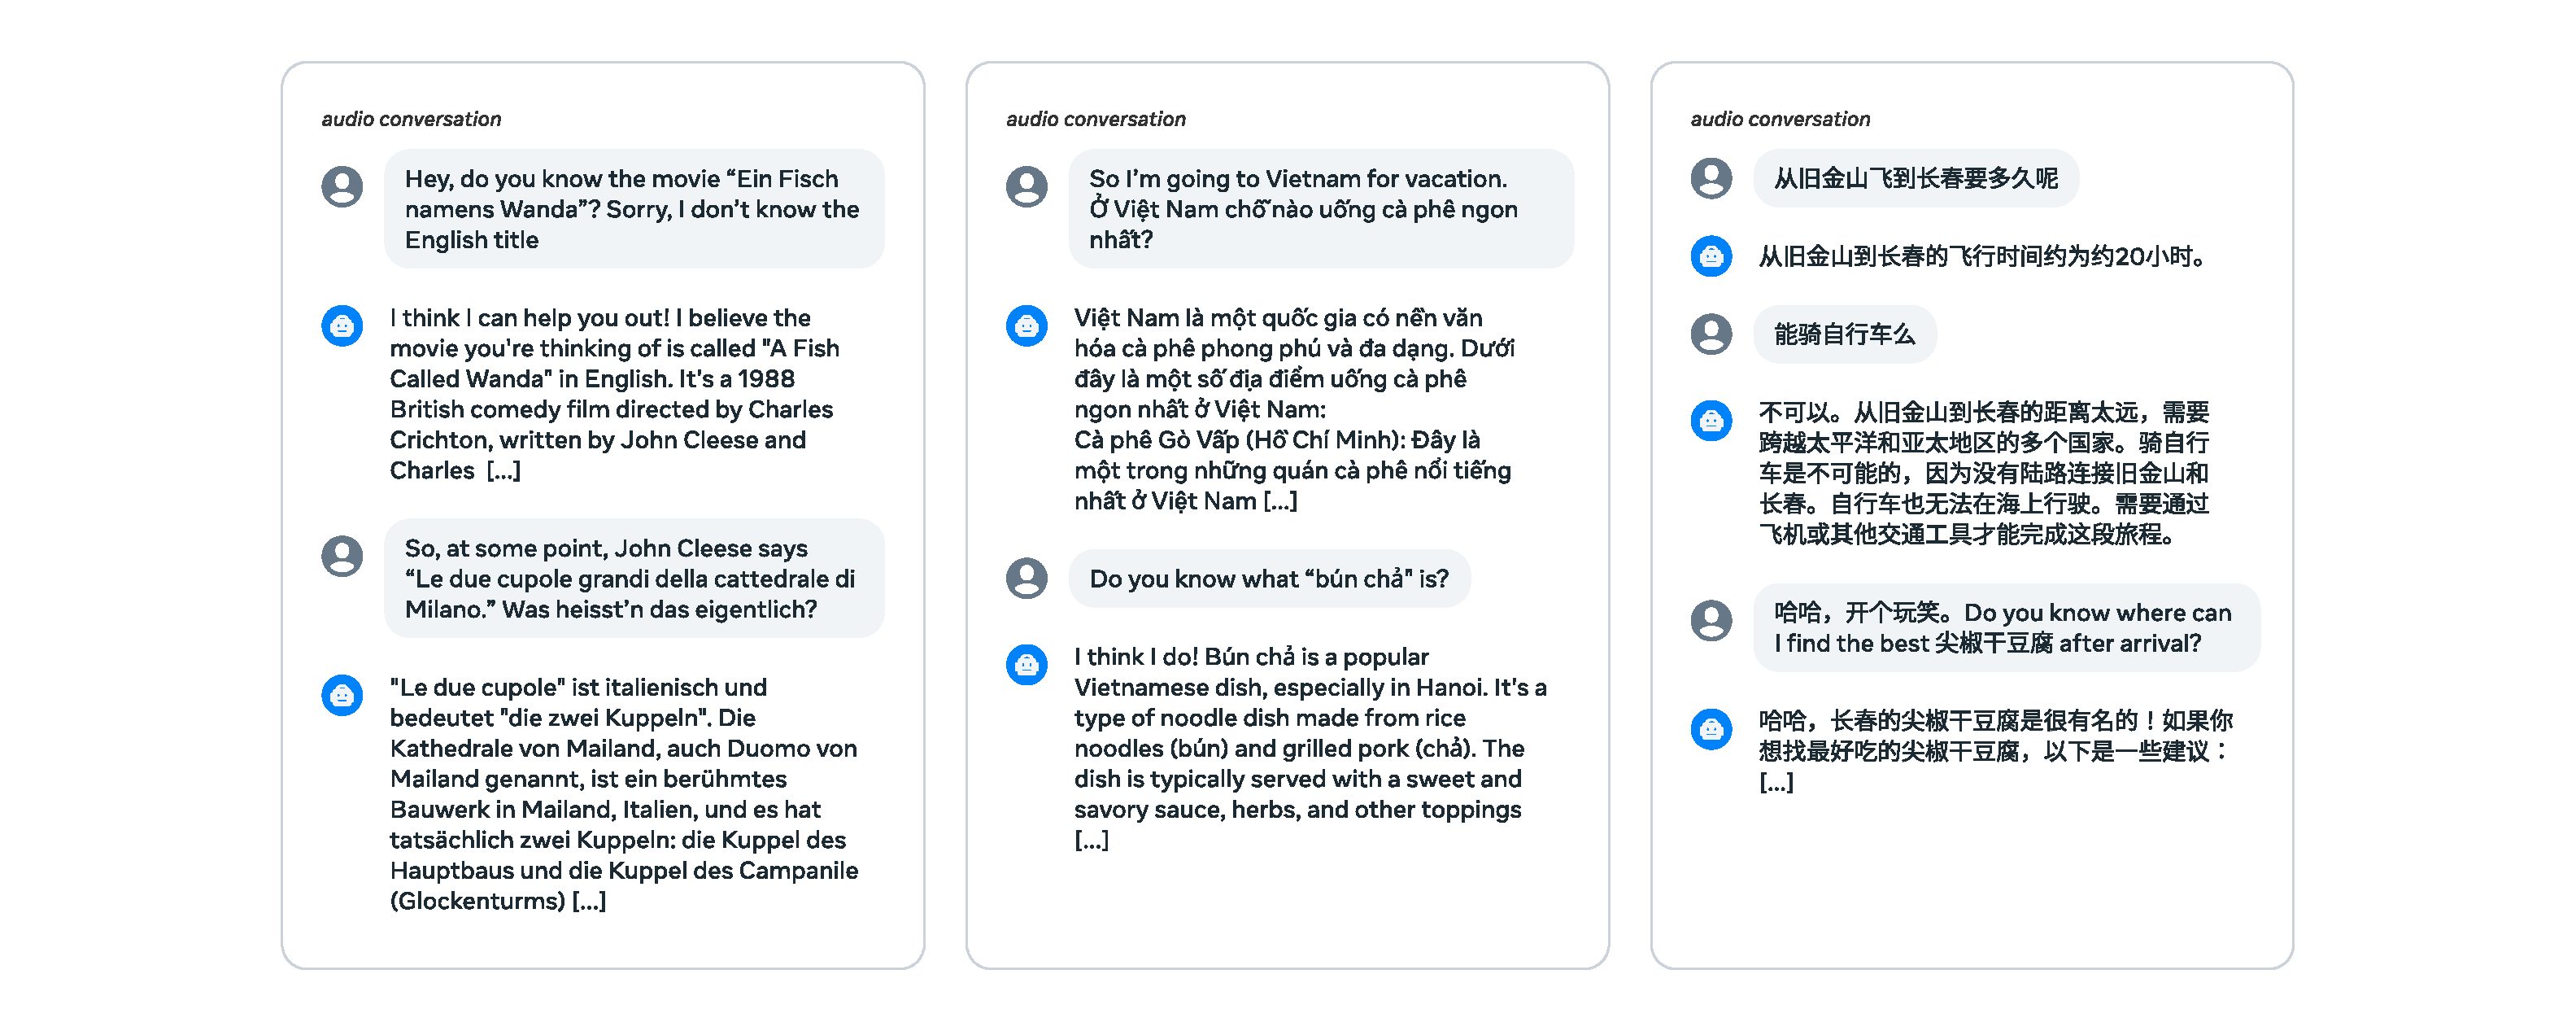
\includegraphics[trim={150px 0 150px 0},clip,width=\textwidth]{assets/llama-voice-language.pdf}
    \caption{\textbf{Transcribed dialogue examples using the speech interface for Llama 3.} The examples illustrate zero-shot multi-turn and code-switching capabilities.}
    \label{figure:speech_dialog_example}
\end{figure}

\textbf{Spoken question answering.}
The speech interface of Llama 3 demonstrates remarkable question answering capabilities. The model can effortlessly comprehend code-switched speech without any prior exposure to such data. Notably, although the model was trained only on single-turn dialogue, it is capable of engaging in extended, coherent multi-turn dialogue sessions.
Figure~\ref{figure:speech_dialog_example} presents a few examples that highlight these multilingual and multi-turn capabilities.

\begin{table}[t]
\centering
    \begin{tabular}{lcccccc}
    \toprule
     & \multicolumn{2}{c}{\textbf{Llama 3 8B}} &  \multicolumn{2}{c}{\textbf{Llama 3 70B}} & \multicolumn{2}{c}{\textbf{Gemini 1.5 Pro}} \\
    \textbf{Language} & AT \bdown & LT \bup & AT \bdown & LT  \bup & AT \bdown & LT \bup \\
    \midrule
    English & 0.84 & 15.09 & \textbf{0.68} & \textbf{15.46} & 1.44 & 13.42 \\
    Overall & 2.31 & 9.89 & \textbf{2.00} & 10.29 & 2.06 & \textbf{10.94} \\
    \bottomrule
    \end{tabular}
    \caption{\textbf{Speech toxicity of our speech interface to Llama 3 on the MuTox dataset.} AT refers to added toxicity (\%) and LT refers to lost toxicity (\%). \label{table:speech-safety-mutox}}
\end{table}

\textbf{Safety.}
We evaluate the safety of our speech model on MuTox \citep{mutox}, a multilingual audio-based dataset of 20,000 utterances for English and Spanish and 4,000 for 19 other languages, each with toxicity labels attached.
The audio is passed as input to the model and the output is evaluated for toxicity, after cleaning some special characters.
We apply the MuTox classifier~\citep{mutox} and compare the results with Gemini 1.5 Pro. We evaluate the percentage of added toxicity (AT), when the input prompt is safe and the output is toxic, and the percentage of lost toxicity (LT), when the input prompt is toxic and the answer is safe. Table~\ref{table:speech-safety-mutox} shows the results for English and an average across all 21 languages that we evaluated on.\footnote{Note that for Gemini, we encountered that a significant number of responses were empty, which could be due to safety filters on their side (though some empty responses were for non-toxic input) or to rate limits. To conduct the analysis, we assumed that all the empty responses are safe. This is the most conservative approach for results and the upper bound of what Gemini results would look like.} The percentage of added toxicity is very low: our speech models have the lowest percentage of added toxicity for English, with less than 1\%. It removes significantly more toxicity than it adds.


\subsection{Speech Generation Results}
For speech generation, we focus on evaluating the quality of token-wise input streaming models with the Llama 3 embeddings for the text normalization and prosody modeling tasks. The evaluation focuses on comparisons with models that do not take the Llama 3 embeddings as an additional input.

\textbf{Text normalization.}
To measure the effect of Llama 3 embeddings, we experimented with changing the amount of right context the model uses. We trained the model using a right context of 3 TN tokens (demarcated by unicode category). This model is compared to models that do not use the Llama 3 embeddings, using a 3-token right context or a full bi-directional context.
As expected, Table~\ref{tab:table1} shows using the full right context improves performance for the model without Llama 3 embeddings. However, the model that incorporates the Llama 3 embeddings outperforms all other models, hence enabling token-rate input/output streaming without relying on long context in the input.

\begin{wraptable}{r}{0.45\textwidth}
	\begin{NiceTabular}{lcc}
		\CodeBefore
		\Body
		\toprule
		\textbf{Model} & \textbf{Context} & \textbf{Accuracy} \\
		\midrule
		Without Llama 3 8B & 3 & 73.6\% \\
		Without Llama 3 8B & $\infty$ & 88.0\% \\
		With Llama 3 8B & 3 & \textbf{90.7\%} \\
		\bottomrule
	\end{NiceTabular}
	\caption{\textbf{Sample-wise text normalization (TN) accuracy.} We compare models with or without Llama 3 8B embeddings, and using different right-context values.\vspace{-8mm}}
	\label{tab:table1}
\end{wraptable}

\textbf{Prosody modeling.}
To evaluate the performance of the our prosody model (PM) with Llama 3 8B, we conducted two sets of human evaluation comparing models with and without Llama 3 embeddings. Raters listened to samples from different models and indicated their preferences. To generate the final speech waveform, we use an in-house transformer based acoustic model \citep{wu2021transformer} that predicts spectral features and a WaveRNN neural vocoder \citep{kalchbrenner2018efficient} to generate the final speech waveform.  %

\begin{table}[t]
	\centering
    \begin{minipage}{.48\textwidth}
      \centering
      \begin{tabular}{lcc}
		\toprule
		\textbf{Model} & \textbf{Preference} \\
		\midrule
		PM for Llama 3 8B  & \textbf{60.0\%} \\
		\small{Streaming phone-only baseline} & 40.0\% \\
		\bottomrule
      \end{tabular}
		\label{tab:tts:pm:ab_test1}
    \end{minipage}\hfill
    \begin{minipage}{.48\textwidth}
      \centering
      \begin{tabular}{lcc}
		\toprule
		\textbf{Model} & \textbf{Preference} \\
		\midrule
		PM for Llama 3 8B & \textbf{63.6\%} \\
		\small{Non-streaming phone-only baseline} & 36.4\% \\
		\bottomrule
      \end{tabular}

    \end{minipage}
    \caption{\textbf{Prosody Modeling (PM) evaluation.} \emph{Left:} Rater preferences of PM for Llama 3 8B vs. streaming phone-only baseline. \emph{Right:} Rater preferences of PM for Llama 3 8B vs. non-streaming phone-only baseline.}
    \label{tab:pm_test}

\end{table}




First, we compare directly to a streaming baseline model without Llama 3 embeddings. 
In  the second test, the Llama 3 8B PM is compared to a non-streaming baseline model without Llama 3 embeddings. 
As shown in Table~\ref{tab:pm_test}, the Llama 3 8B PM is preferred  60\% of the time compared to the streaming baseline, and 63.6\% of the time  compared to the non-streaming baseline, indicating a significant improvement in perceived quality. The key advantage of the Llama 3 8B PM is its token-wise streaming capability (Section~\ref{sec:tts:pm}), which maintains low latency during inference. This reduces the model's lookahead requirements, enabling more responsive and real-time speech synthesis compared to non-streaming baselines.
Overall, the Llama 3 8B prosody model consistently outperforms the baseline models, demonstrating its effectiveness in enhancing the naturalness and expressiveness of synthesized speech.

\section{Related Work}
\label{section:related_work}
The development of Llama 3 builds on a large body of prior work studying foundation models for language, images, videos, and speech.
A comprehensive overview of that work is outside the scope of this paper; we refer the reader to \citet{bordes2024vlm,madan2024foundation,LLMSurvey} for such overviews.
Below, we briefly outline seminal works that directly influenced the development of Llama 3.

\subsection{Language}
\label{section:related_work_language}

\textbf{Scale.}
Llama 3 follows the enduring trend of applying straightforward methods at ever increasing scales in foundation models. Improvements are driven by increased compute and improved data, with the 405B model using almost fifty times the pre-training compute budget of Llama 2 70B. Despite containing 405B parameters, our largest Llama 3 in fact contains fewer parameters than earlier and much less performant models such as PALM~\citep{chowdhery2023palm}, due to better understanding of scaling laws~\citep{kaplan2020scaling,hoffmann2022chinchilla}. Little is publicly known about the size of other frontier models, such as Claude 3 or GPT 4~\citep{openai2023gpt4}, but overall performance is compareable. 

\textbf{Small models.}
Developments in smaller models have paralleled those in large models. 
Models with fewer parameters can dramatically improve inference cost and simplify deployment~\citep{mehta2024openelm,team2024gemma}.
The smaller Llama 3 models achieve this by training far beyond the point of compute optimal training, effectively trading training compute for inference efficiency.
An alternative path is to distill larger models into smaller ones, as in Phi~\citep{abdin2024phi}.

\textbf{Architectures.}
While Llama 3 makes minimal architectural modifiations to compared to Llama 2, other recent foundation models have explored other designs. Most notably, mixture of experts architectures~\citep{shazeer2017moe,lewis2021base,fedus2022switch,zhou2022mixture} can be used as an efficient way to increase the capacity of a models, such as in Mixtral~\citep{jiang2024mixtral} and Arctic~\citep{snowflakearctic}. Llama 3 outperforms these models, suggesting that dense architectures are not the limiting factor, but there remain numerous trade offs in terms of training and inference efficiency, and model stability at scale.

\textbf{Open source.}
Open weights foundation models have rapidly improved over the last year, with Llama3-405B now competitive with the current closed weight state-of-the-art. 
Numerous model families have recently been developed, including Mistral~\citep{jiang2023mistral}, Falcon~\citep{almazrouei2023falcon}, MPT~\citep{databricksmpt}, Pythia~\citep{biderman2023pythia}, Arctic~\citep{snowflakearctic}, OpenELM~\citep{mehta2024openelm}, OLMo~\citep{groeneveld2024olmoacceleratingsciencelanguage}, StableLM~\citep{bellagente2024stable}, OpenLLaMA~\citep{openlm2023openllama}, Qwen~\citep{bai2023qwen}, Gemma~\citep{team2024gemma}, Grok~\citep{xaigrok}, and Phi~\citep{abdin2024phi}.

\textbf{Post-training.}
Post-training \llamathree follows the established strategy of instruction tuning~\citep{chung2022scalinginstruction,ouyang2022instructgpt} followed by alignment with human feedback~\citep{kaufmann2023survey}. While some studies have shown the surprising effectiveness of lightweight alignment procedures~\citep{zhou2024lima}, \llamathree uses millions of human instructions and preference judgments to improve the pre-trained model, including techniques such as rejection sampling~\citep{constitutional-ai-bai}, supervised finetuning~\citep{sanh2022multitask}, and Direct Preference Optimization~\citep{rafailov2023dpo}. In order to curate these instruction and preference examples, we deploy earlier versions of \llamathree to filter~\citep{liu2024makesgooddataalignment}, re-write~\citep{pan2024selfcorrection}, or generate prompts and responses~\citep{liu2024bestpractices} and apply these techniques through multiple rounds of post-training.


\subsection{Multimodality}
\label{section:related_work_multimodality}
Our experiments with multimodal capabilities for Llama 3 are part of a long line of work on foundation models that jointly model multiple modalities.

\textbf{Images.} 
A substantial body of work has trained image-recognition models on large amounts of image-text pairs, for example, \citet{Mahajan_2018_ECCV,xiao2024florence,chameleon2024,openai2023gpt4blog}.
\citet{radford2021learning} presented one of the first models to jointly embed images and text via contrastive learning. 
More recently, a series of models has studied approaches similar to the one used in Llama 3, for example, \citet{alayrac2022flamingo,dai2023instructblip,liu2023llava,liu2023improvedllava,yang2023mmreact,ye2023mplug,zhu2023minigpt}.
Our approach in Llama 3 combines ideas from many of these papers to achieve results that are comparable with Gemini 1.0 Ultra \citep{gemini2023gemini} and GPT-4 Vision \citep{openai2023gpt4blog}; see Section~\ref{section:results_image_recognition}.


\textbf{Video.}
Although video inputs are supported by an increasing number of foundation models \citep{gemini2023gemini,openai2023gpt4blog}, the body of work on joint modeling of videos and language is not that large.
Akin to Llama 3, most current studies adopt an adapter approach to align video and language representations and unlock question-answering and reasoning about videos \citep{lin2023video,li2023videochat,Maaz2023VideoChatGPT,zhang2023videollama,zhao2022lavila}.
We find that such approaches produce results that are competitive with the state-of-the-art; see Section~\ref{section:results_video_recognition}.

\textbf{Speech.}
Our work also fits in a larger body of work combining language and speech modeling.
Earlier joint models of text and speech include AudioPaLM \citep{rubenstein2023audiopalm}, VioLA \citep{wang2023viola}, VoxtLM \cite{maiti2023voxtlm}, SUTLM \citep{chou2023sutlm}, and Spirit-LM \citep{nguyen2024spirit}.
Our work builds on prior compositional approaches to combining speech and language like \citet{fathullah2024audiochatllama}.
Unlike most prior work, we opt to not finetune the language model itself for speech tasks as doing so may lead to contention on non-speech tasks.
We find that at larger model scales, strong performances are attainable even without such finetuning; see Section~\ref{section:results_speech}.



Hyperbolic embeddings embed hierarchical information with high
fidelity and few dimensions. We explored the limits of this approach
by describing scalable, high quality algorithms. We hope the
techniques here encourage more follow-on work on the exciting
techniques of \citet{fb, ucl}. As future work, we hope to explore how
hyperbolic embeddings can be most effectively incorporated into downstream
tasks and applications.


\clearpage
\section*{Contributors and Acknowledgements}
Llama 3 is the result of the work of a large number of people at Meta.
Below, we list all \textbf{core contributors} (people who worked on Llama 3 for at least $\nicefrac{2}{3}$rd of the runtime of the project) and \textbf{contributors} (people who worked on Llama 3 for at least $\nicefrac{1}{5}$th of the runtime of the project).
We list all contributors in alphabetical order of first name.

\subsection*{Core Contributors}
Aaron Grattafiori, Abhimanyu Dubey, Abhinav Jauhri, Abhinav Pandey, Abhishek Kadian, Ahmad Al-Dahle, Aiesha Letman, Akhil Mathur, Alan Schelten, Alex Vaughan, Amy Yang, Angela Fan, Anirudh Goyal, Anthony Hartshorn, Aobo Yang, Archi Mitra, Archie Sravankumar, Artem Korenev, Arthur Hinsvark, Arun Rao, Aston Zhang, Aurelien Rodriguez, Austen Gregerson, Ava Spataru, Baptiste Roziere, Bethany Biron, Binh Tang, Bobbie Chern, Charlotte Caucheteux, Chaya Nayak, Chloe Bi, Chris Marra, Chris McConnell, Christian Keller, Christophe Touret, Chunyang Wu, Corinne Wong, Cristian Canton Ferrer, Cyrus Nikolaidis, Damien Allonsius, Daniel Song, Danielle Pintz, Danny Livshits, Danny Wyatt, David Esiobu, Dhruv Choudhary, Dhruv Mahajan, Diego Garcia-Olano, Diego Perino, Dieuwke Hupkes, Egor Lakomkin, Ehab AlBadawy, Elina Lobanova, Emily Dinan, Eric Michael Smith, Filip Radenovic, Francisco Guzmán, Frank Zhang, Gabriel Synnaeve, Gabrielle Lee, Georgia Lewis Anderson, Govind Thattai, Graeme Nail, Gregoire Mialon, Guan Pang, Guillem Cucurell, Hailey Nguyen, Hannah Korevaar, Hu Xu, Hugo Touvron, Iliyan Zarov, Imanol Arrieta Ibarra, Isabel Kloumann, Ishan Misra, Ivan Evtimov, Jack Zhang, Jade Copet, Jaewon Lee, Jan Geffert, Jana Vranes, Jason Park, Jay Mahadeokar, Jeet Shah, Jelmer van der Linde, Jennifer Billock, Jenny Hong, Jenya Lee, Jeremy Fu, Jianfeng Chi, Jianyu Huang, Jiawen Liu, Jie Wang, Jiecao Yu, Joanna Bitton, Joe Spisak, Jongsoo Park, Joseph Rocca, Joshua Johnstun, Joshua Saxe, Junteng Jia, Kalyan Vasuden Alwala, Karthik Prasad, Kartikeya Upasani, Kate Plawiak, Ke Li, Kenneth Heafield, Kevin Stone, Khalid El-Arini, Krithika Iyer, Kshitiz Malik, Kuenley Chiu, Kunal Bhalla, Kushal Lakhotia, Lauren Rantala-Yeary, Laurens van der Maaten, Lawrence Chen, Liang Tan, Liz Jenkins, Louis Martin, Lovish Madaan, Lubo Malo, Lukas Blecher, Lukas Landzaat, Luke de Oliveira, Madeline Muzzi, Mahesh Pasupuleti, Mannat Singh, Manohar Paluri, Marcin Kardas, Maria Tsimpoukelli, Mathew Oldham, Mathieu Rita, Maya Pavlova, Melanie Kambadur, Mike Lewis, Min Si, Mitesh Kumar Singh, Mona Hassan, Naman Goyal, Narjes Torabi, Nikolay Bashlykov, Nikolay Bogoychev, Niladri Chatterji, Ning Zhang, Olivier Duchenne, Onur Çelebi, Patrick Alrassy, Pengchuan Zhang, Pengwei Li, Petar Vasic, Peter Weng, Prajjwal Bhargava, Pratik Dubal, Praveen Krishnan, Punit Singh Koura, Puxin Xu, Qing He, Qingxiao Dong, Ragavan Srinivasan, Raj Ganapathy, Ramon Calderer, Ricardo Silveira Cabral, Robert Stojnic, Roberta Raileanu, Rohan Maheswari, Rohit Girdhar, Rohit Patel, Romain Sauvestre, Ronnie Polidoro, Roshan Sumbaly, Ross Taylor, Ruan Silva, Rui Hou, Rui Wang, Saghar Hosseini, Sahana Chennabasappa, Sanjay Singh, Sean Bell, Seohyun Sonia Kim, Sergey Edunov, Shaoliang Nie, Sharan Narang, Sharath Raparthy, Sheng Shen, Shengye Wan, Shruti Bhosale, Shun Zhang, Simon Vandenhende, Soumya Batra, Spencer Whitman, Sten Sootla, Stephane Collot, Suchin Gururangan, Sydney Borodinsky, Tamar Herman, Tara Fowler, Tarek Sheasha, Thomas Georgiou, Thomas Scialom, Tobias Speckbacher, Todor Mihaylov, Tong Xiao, Ujjwal Karn, Vedanuj Goswami, Vibhor Gupta, Vignesh Ramanathan, Viktor Kerkez, Vincent Gonguet, Virginie Do, Vish Vogeti, Vítor Albiero, Vladan Petrovic, Weiwei Chu, Wenhan Xiong, Wenyin Fu, Whitney Meers, Xavier Martinet, Xiaodong Wang, Xiaofang Wang, Xiaoqing Ellen Tan, Xide Xia, Xinfeng Xie, Xuchao Jia, Xuewei Wang, Yaelle Goldschlag, Yashesh Gaur, Yasmine Babaei, Yi Wen, Yiwen Song, Yuchen Zhang, Yue Li, Yuning Mao, Zacharie Delpierre Coudert, Zheng Yan, Zhengxing Chen, and Zoe Papakipos.

\subsection*{Contributors}
Aaditya Singh, Aayushi Srivastava, Abha Jain, Adam Kelsey, Adam Shajnfeld, Adithya Gangidi, Adolfo Victoria, Ahuva Goldstand, Ajay Menon, Ajay Sharma, Alex Boesenberg, Alexei Baevski, Allie Feinstein, Amanda Kallet, Amit Sangani, Amos Teo, Anam Yunus, Andrei Lupu, Andres Alvarado, Andrew Caples, Andrew Gu, Andrew Ho, Andrew Poulton, Andrew Ryan, Ankit Ramchandani, Annie Dong, Annie Franco, Anuj Goyal, Aparajita Saraf, Arkabandhu Chowdhury, Ashley Gabriel, Ashwin Bharambe, Assaf Eisenman, Azadeh Yazdan, Beau James, Ben Maurer, Benjamin Leonhardi, Bernie Huang, Beth Loyd, Beto De Paola, Bhargavi Paranjape, Bing Liu, Bo Wu, Boyu Ni, Braden Hancock, Bram Wasti, Brandon Spence, Brani Stojkovic, Brian Gamido, Britt Montalvo, Carl Parker, Carly Burton, Catalina Mejia, Ce Liu, Changhan Wang, Changkyu Kim, Chao Zhou, Chester Hu, Ching-Hsiang Chu, Chris Cai, Chris Tindal, Christoph Feichtenhofer, Cynthia Gao, Damon Civin, Dana Beaty, Daniel Kreymer, Daniel Li,  David Adkins, David Xu, Davide Testuggine, Delia David, Devi Parikh, Diana Liskovich, Didem Foss, Dingkang Wang, Duc Le, Dustin Holland, Edward Dowling, Eissa Jamil, Elaine Montgomery, Eleonora Presani, Emily Hahn, Emily Wood, Eric-Tuan Le, Erik Brinkman, Esteban Arcaute, Evan Dunbar, Evan Smothers, Fei Sun, Felix Kreuk, Feng Tian, Filippos Kokkinos, Firat Ozgenel, Francesco Caggioni, Frank Kanayet, Frank Seide, Gabriela Medina Florez, Gabriella Schwarz, Gada Badeer, Georgia Swee, Gil Halpern, Grant Herman, Grigory Sizov, Guangyi (Jack) Zhang, Guna Lakshminarayanan, Hakan Inan, Hamid Shojanazeri, Han Zou, Hannah Wang, Hanwen Zha, Haroun Habeeb, Harrison Rudolph, Helen Suk, Henry Aspegren, Hunter Goldman, Hongyuan Zhan, Ibrahim Damlaj, Igor Molybog, Igor Tufanov, Ilias Leontiadis, Irina-Elena Veliche, Itai Gat, Jake Weissman, James Geboski, James Kohli, Janice Lam, Japhet Asher, Jean-Baptiste Gaya, Jeff Marcus, Jeff Tang, Jennifer Chan, Jenny Zhen, Jeremy Reizenstein, Jeremy Teboul, Jessica Zhong, Jian Jin, Jingyi Yang, Joe Cummings, Jon Carvill, Jon Shepard, Jonathan McPhie, Jonathan Torres, Josh Ginsburg, Junjie Wang, Kai Wu, Kam Hou U, Karan Saxena, Kartikay Khandelwal, Katayoun Zand, Kathy Matosich, Kaushik Veeraraghavan, Kelly Michelena, Keqian Li, Kiran Jagadeesh, Kun Huang, Kunal Chawla, Kyle Huang, Lailin Chen, Lakshya Garg, Lavender A, Leandro Silva, Lee Bell, Lei Zhang, Liangpeng Guo, Licheng Yu, Liron Moshkovich, Luca Wehrstedt, Madian Khabsa, Manav Avalani, Manish Bhatt, Martynas Mankus, Matan Hasson, Matthew Lennie, Matthias Reso, Maxim Groshev, Maxim Naumov, Maya Lathi, Meghan Keneally, Miao Liu, Michael L. Seltzer, Michal Valko, Michelle Restrepo, Mihir Patel, Mik Vyatskov, Mikayel Samvelyan, Mike Clark, Mike Macey, Mike Wang, Miquel Jubert Hermoso, Mo Metanat, Mohammad Rastegari, Munish Bansal, Nandhini Santhanam, Natascha Parks, Natasha White, Navyata Bawa, Nayan Singhal, Nick Egebo, Nicolas Usunier, Nikhil Mehta, Nikolay Pavlovich Laptev, Ning Dong, Norman Cheng, Oleg Chernoguz, Olivia Hart, Omkar Salpekar, Ozlem Kalinli, Parkin Kent, Parth Parekh, Paul Saab, Pavan Balaji, Pedro Rittner, Philip Bontrager, Pierre Roux, Piotr Dollar, Polina Zvyagina, Prashant Ratanchandani, Pritish Yuvraj, Qian Liang, Rachad Alao, Rachel Rodriguez, Rafi Ayub, Raghotham Murthy, Raghu Nayani, Rahul Mitra, Rangaprabhu Parthasarathy, Raymond Li, Rebekkah Hogan, Robin Battey, Rocky Wang, Russ Howes, Ruty Rinott, Sachin Mehta, Sachin Siby, Sai Jayesh Bondu, Samyak Datta, Sara Chugh, Sara Hunt, Sargun Dhillon, Sasha Sidorov, Satadru Pan, Saurabh Mahajan, Saurabh Verma, Seiji Yamamoto, Sharadh Ramaswamy, Shaun Lindsay, Shaun Lindsay, Sheng Feng, Shenghao Lin, Shengxin Cindy Zha, Shishir Patil, Shiva Shankar, Shuqiang Zhang, Shuqiang Zhang, Sinong Wang, Sneha Agarwal, Soji Sajuyigbe, Soumith Chintala, Stephanie Max, Stephen Chen, Steve Kehoe, Steve Satterfield, Sudarshan Govindaprasad, Sumit Gupta, Summer Deng, Sungmin Cho, Sunny Virk, Suraj Subramanian, Sy Choudhury, Sydney Goldman, Tal Remez, Tamar Glaser, Tamara Best, Thilo Koehler, Thomas Robinson, Tianhe Li, Tianjun Zhang, Tim Matthews, Timothy Chou, Tzook Shaked, Varun Vontimitta, Victoria Ajayi, Victoria Montanez, Vijai Mohan, Vinay Satish Kumar, Vishal Mangla, Vlad Ionescu, Vlad Poenaru, Vlad Tiberiu Mihailescu, Vladimir Ivanov, Wei Li, Wenchen Wang, Wenwen Jiang, Wes Bouaziz, Will Constable, Xiaocheng Tang, Xiaojian Wu, Xiaolan Wang, Xilun Wu, Xinbo Gao, Yaniv Kleinman, Yanjun Chen, Ye Hu, Ye Jia, Ye Qi, Yenda Li, Yilin Zhang, Ying Zhang, Yossi Adi, Youngjin Nam, Yu (Sid) Wang, Yu Zhao, Yuchen Hao, Yundi Qian, Yunlu Li, Yuzi He, Zach Rait, Zachary DeVito, Zef Rosnbrick, Zhaoduo Wen, Zhenyu Yang, Zhiwei Zhao, and Zhiyu Ma.

\subsection*{Acknowledgements}
We thank Mark Zuckerberg, Chris Cox, Ahmad Al-Dahle, Santosh Janardhan, Joelle Pineau, Yann LeCun, Aparna Ramani, Yee Jiun Song, and Ash Jhaveri for their invaluable support for Llama 3.

We also thank Aasish Pappu, Adebissy Tharinger, Adnan Aziz, Aisha Iqbal, Ajit Mathews, Albert Lin, Amar Budhiraja, Amit Nagpal, Andrew Or, Andrew Prasetyo Jo, Ankit Jain, Antonio Prado, Aran Mun, Armand Kok, Ashmitha Jeevaraj Shetty, Aya Ibrahim, Bardiya Sadeghi, Beibei Zhu, Bell Praditchai, Benjamin Muller, Botao Chen, Carmen Wang, Carolina Tsai, Cen Peng, Cen Zhao, Chana Greene, Changsheng Zhao, Chenguang Zhu, Chloé Bakalar, Christian Fuegen, Christophe Ropers, Christopher Luc, Dalton Flanagan, Damien Sereni, Dan Johnson, Daniel Haziza, Daniel Kim, David Kessel, Digant Desai, Divya Shah, Dong Li, Elisabeth Michaels, Elissa Jones, Emad El-Haraty, Emilien Garreau, Eric Alamillo, Eric Hambro, Erika Lal, Eugen Hotaj, Fabian Gloeckle, Fadli Basyari, Faith Eischen, Fei Kou, Ferdi Adeputra, Feryandi Nurdiantoro, Flaurencya Ciputra, Forest Zheng, Francisco Massa, Furn Techaletumpai, Gobinda Saha, Gokul Nadathur, Greg Steinbrecher, Gregory Chanan, Guille Cobo, Guillem Brasó, Hany Morsy, Haonan Sun, Hardik Shah, Henry Erksine Crum, Hongbo Zhang, Hongjiang Lv, Hongye Yang, Hweimi Tsou, Hyunbin Park, Ian Graves, Jack Wu, Jalpa Patel, James Beldock, James Zeng, Jeff Camp, Jesse He, Jilong Wu, Jim Jetsada Machom, Jinho Hwang, Jonas Gehring, Jonas Kohler, Jose Leitao, Josh Fromm, Juan Pino, Julia Rezende, Julian Garces, Kae Hansanti, Kanika Narang, Kartik Khandelwal, Keito Uchiyama, Kevin McAlister, Kimish Patel, Kody Bartelt, Kristina Pereyra, Kunhao Zheng, Lien Thai, Lu Yuan, Lunwen He, Marco Campana, Mariana Velasquez, Marta R. Costa-jussa, Martin Yuan, Max Ren, Mayank Khamesra, Mengjiao MJ Wang, Mengqi Mu, Mergen Nachin, Michael Suo, Mikel Jimenez Fernandez, Mustafa Ozdal, Na Li, Nahiyan Malik, Naoya Miyanohara, Narges Torabi, Nathan Davis, Nico Lopero, Nikhil Naik, Ning Li, Octary Azis, PK Khambanonda, Padchara Bubphasan, Pian Pawakapan, Prabhav Agrawal, Praveen Gollakota, Purin Waranimman, Qian Sun, Quentin Carbonneaux, Rajasi Saha, Rhea Nayak, Ricardo Lopez-Barquilla, Richard Huang, Richard Qiu, Richard Tosi, Rishi Godugu, Rochit Sapra, Rolando Rodriguez Antunez, Ruihan Shan, Sakshi Boolchandani, Sam Corbett-Davies, Samuel Djunaedi, Sarunya Pumma, Saskia Adams, Scott Wolchok, Shankar Kalyanaraman, Shashi Gandham, Shengjie Bi, Shengxing Cindy, Shervin Shahidi, Sho Yaida, Shoubhik Debnath, Sirirut Sonjai, Srikanth Sundaresan, Stephanie Worland, Susana Contrera, Tejas Shah, Terry Lam, Tony Cao, Tony Lee, Tristan Rice, Vishy Poosala, Wenyu Chen, Wesley Lee, William Held, Xiaozhu Meng, Xinhua Wang, Xintian Wu, Yanghan Wang, Yaroslava Kuzmina, Yifan Wang, Yuanhao Xiong, Yue Zhao, Yun Wang, Zaibo Wang, Zechun Liu, and Zixi Qi for helpful contributions to Llama 3.


\clearpage
\newpage
\bibliographystyle{assets/plainnat}
\bibliography{paper,anthology}



\end{document}
